%\documentclass[unicode,master]{scutthesis} % 草稿封面,硕士则添加选项master,博士则去掉。使用正式封面时注释该行
 \documentclass[unicode,master,pdfcover]{scutthesis} %   % 论文正式封面,pdfcover为可选项,终稿再添加,使用草稿封面时注释该行
\usepackage{array,longtable,graphicx} 
\usepackage{anyfontsize} %消除字体警告
\usepackage{enumitem}
\usepackage{makecell}
\usepackage[colorinlistoftodos,backgroundcolor=yellow]{todonotes} % 黄色背景+目录显示[5](@ref)
\usepackage{multicol} % 导言区引入
\usepackage{siunitx} % 单位排版
\usepackage{bm} % 添加bm包支持\bm命令

%%%%%%%%%%%%%%%%%%%%%%%%%%%%%%%%%%%%%%%%%%%%%%%%%%%%%%%%%%%%%%%%%%%%%%%%%%%%%%%%%%——by MCH
%编译范围
% \includeonly{chapter/chapter04}
%参考文献设置
\usepackage[backend=biber,style=gb7714-2015,gbalign=gb7714-2015,gbpub=false,gbnamefmt = lowercase,gbpunctin=false]{biblatex}% 可试着设style=gb7714-2015
\addbibresource[location=local]{biblibrary/jichuliubian.bib} 
\addbibresource[location=local]{biblibrary/shuzhimoni.bib} 
\addbibresource[location=local]{biblibrary/deepbengou.bib}
\addbibresource[location=local]{biblibrary/deeplearning.bib}
\DefineBibliographyStrings{english}{in={}}
\DefineBibliographyStrings{english}{incn={}}
% % 自定义相关引用格式,去掉 “In: Springer US.”
% \renewbibmacro{in:}{%
%   \printtext{\bibstring{}}%
%   \clearfield{institution}%
%   \clearname{editor}%
%   \clearfield{series}%
%   \clearfield{publisher}%
%   \clearfield{location}%
%   \newunit}

% % 自定义 inproceedings 和 inbook 的相关引用格式
% \renewbibmacro*{related:inproceedings}{%
%   \entrydata*{\relatedentry}{%
%     \usedriver{}{\thefield{entrytype}}%
%     \newunit}}

% \renewbibmacro*{related:inbook}{%
%   \entrydata*{\relatedentry}{%
%     \usedriver{}{\thefield{entrytype}}%
%     \newunit}}

% % 自定义 relatedstring 格式
% \DeclareFieldFormat{relatedstring:inproceedings}{}
% \DeclareFieldFormat{relatedstring:inbook}{}

% % 移除析出文献中的 “In: Springer US.”
% \renewbibmacro{cite:inproceedings}{%
%   \usebibmacro{cite:author}%
%   \setunit{\addcomma\space}%
%   \usebibmacro{cite:title}%
%   \setunit{\addcomma\space}%
%   \usebibmacro{cite:journal+issuetitle}%
%   \newunit}
%页眉页脚设置
\usepackage{fancyhdr}
\usepackage{listings}
\usepackage{xunicode}
\renewcommand{\lstlistingname}{列表}
\pagestyle{fancy}
\fancyfoot[C]{\headfont\thepage}
\renewcommand{\chaptermark}[1]{\markboth{\chaptername\ #1}{}}
\renewcommand{\sectionmark}[1]{\markright{\thesection\ #1}}
\fancyhead[RE]{}
\fancyhead[RO]{}

\fancyhead[LE]{}
\fancyhead[LO]{}
\fancyhead[CO]{\headfont{\leftmark}}
\fancyhead[CE]{\headfont{华南理工大学硕士学位论文}}% 
\renewcommand{\headrulewidth}{1.5pt}
\renewcommand{\footrulewidth}{0pt}
%%%%%%%%%%%%%%%%%%%%%%%%%%%%%%%%%%%%%%%%%%%%%%%%%%%%%%%%%%%%%%%%%%%%%%%%%%%%%%%%%%
% \usepackage[unicode=true,bookmarks=true,bookmarksnumbered=true,bookmarksopen=false,breaklinks=false,pdfborder={0 0 1},backref=false,colorlinks=true]{hyperref}
\usepackage[unicode=true, bookmarks=true, bookmarksnumbered=true, pdfborder={0 0 1}, colorlinks=true, linkcolor=black, citecolor=black, urlcolor=black]{hyperref}

\hypersetup{pdftitle={LaTeX模板使用说明},
	pdfauthor={姓名},
	pdfsubject={华南理工大学硕士学位论文},
%%	pdfsubject={华南理工大学博士学位论文},
	pdfkeywords={PDF关键字1;PDF关键字2},
		linkcolor=black, anchorcolor=black, citecolor=black, filecolor=black, menucolor=black, urlcolor=black, pdfstartview=FitH}% 黑白,提交版
	% linkcolor=blue, anchorcolor=black, citecolor=red, filecolor=magenta, menucolor=red, urlcolor=magenta, pdfstartview=FitH}% 彩色

\makeatletter
%%%%%%%%%%%%%%%%%%%%%%%%%%%%%% LyX specific LaTeX commands.
\providecommand{\LyX}{\texorpdfstring%
	{L\kern-.1667em\lower.25em\hbox{Y}\kern-.125emX\@}
	{LyX}}
%% Because html converters don't know tabularnewline
\providecommand{\tabularnewline}{\\}
\makeatother
\begin{document}
%%%%%%%%%%%%%草稿封面设置%%%%%%%%%%%%%使用“正式封面”时不需要理会这部分
\title{LaTeX模板使用说明}
\author{redfu}
\supervisor{指导教师:周嘉嘉\ 教授}
\institute{华南理工大学}
\date{2025年4月4日}
%%%%%%%%%%%%%%%%%%%%%%%%%%%%%%%%%%%%%

\maketitle

\includepdf[pages=-]{cover_file/yuanchuang.pdf}
\frontmatter	%此后为罗马数字页码,页面类型为plain
\chapter{摘\texorpdfstring{\quad}{}要}
流变学是研究物质变形和流动的科学,流变学本构方程作为其核心内容之一,是描述材料在外力作用下变形和流动行为的数学模型。传统本构方程的获取和研究方法主要依赖实验测定、理论推导和数值模拟,这些方法存在成本高、耗时长、难以泛化等问题,难以满足现代材料科学对高效、精确建模的需求。

近年来,基于数据驱动的机器学习方法开始应用于流变学本构方程的构建研究中,为解决传统方法的局限性提供了新思路。然而,当前的机器学习本构建模方法仍存在物理约束不足、未充分考虑流变学本构方程的历史依赖性、特征稀疏以及难以反推制备参数等问题。

针对上述问题,本文从时间域流变数据建模和频域数据建模两个方向展开研究。在时间域应力应变数据方面,本文创新性地提出物理信息门控循环单元(Physics-Informed Gated Recurrent Unit, PI-GRU)进行时变本构数据的预测建模,利用GRU的门控机制有效捕捉流变学中的记忆效应和应变历史依赖性,同时将物理残差引入损失函数,增强模型的物理约束。相比传统深度前馈神经网络,PI-GRU在经典本构方程的数值模拟数据和真实流变学实验数据上均展现出更优的预测精度和泛化能力。

在频域数据方面,本文采用物理信息神经网络(Physics-Informed Neural Networks, PINN)对材料的制备参数与储存模量、损耗模量、损耗角正切等频域特性关系进行正向建模,通过在损失函数中融入经典本构方程残差,为模型提供物理约束。针对实验中多个制备参数作为特征时出现的稀疏性和分散性问题,本文引入注意力特征融合方法进行特征降维,进一步提升了模型性能。此外,本文应用条件变分自编码器(Conditional Variational Autoencoder, CVAE)对实验数据进行反向建模,实现了从特定流变学性质数据生成实验制备参数的逆向设计。通过构建PINN-CVAE正逆向联合建模框架,为高分子材料的设计提供了高效的辅助支持工具。
\keywordsCN{流变学;本构方程;循环神经网络;物理信息神经网络}

\chapter{Abstract}
Rheology is the scientific study of the deformation and flow of matter. Rheological constitutive equations serve as mathematical models that describe material behavior under external forces. Traditional approaches to developing these equations rely primarily on experimental measurements, theoretical derivation, and numerical simulation. However, these methods face significant limitations including high costs, time-consuming processes, and poor generalizability, making them inadequate for modern materials science demands.

In recent years, data-driven machine learning methods have emerged as promising alternatives for constructing rheological constitutive equations, providing new approaches to overcome the limitations of traditional methods. However, current machine learning approaches still face several challenges, including insufficient physical constraints, inadequate consideration of history-dependent properties in rheological systems, feature sparsity issues, and difficulties in reverse-engineering processing parameters.

To address these challenges, this dissertation explores both time-domain and frequency-domain rheological data modeling approaches. For time-domain stress-strain data, we propose a novel Physics-Informed Gated Recurrent Unit (PI-GRU) framework that effectively captures memory effects and strain-history dependencies through its gating mechanism, while incorporating physical residuals in the loss function to enhance physical constraints. Compared to traditional deep feedforward neural networks, our PI-GRU demonstrates superior predictive accuracy and generalization capabilities on both classical constitutive equation simulations and real rheological experimental data.

For frequency-domain modeling, we employ Physics-Informed Neural Networks (PINNs) to characterize relationships between material processing parameters and frequency-domain properties, including storage modulus, loss modulus, and loss tangent. We incorporate classical constitutive equation residuals as physical constraints to enhance model reliability. To address the sparsity and dispersion challenges associated with multiple processing parameters, we implement an attention-based feature fusion approach for dimensionality reduction, significantly enhancing model performance. Additionally, we develop a Conditional Variational Autoencoder (CVAE) for inverse modeling, enabling reverse design from rheological properties to processing parameters. The resulting PINN-CVAE bidirectional modeling framework provides an efficient tool for polymer material design and optimization.
\keywordsEN{Rheology; Constitutive Equation; Recurrent Neural Network; Physics-Informed Neural Network} % 中英文摘要
%%%%%%%%%%%%%%%%%%%%%%%%%%%%%%%%%%%%%%%%%%%%%%%%
% 目录、表格目录、插图目录这几个字本身的大纲级别是一级的,即和章名有相同的字号字体。目录表的内容通过titletoc宏包在。cls文件设置了。
%\cleardoublepage % pdfbookmark可能需要这一条才能正常工作
\pdfbookmark{\contentsname}{toc} %为目录添加pdf文件书签
\tableofcontents	%目录
\chapter{英文缩略词}
\begin{longtable}{lll}
	\\
	\multicolumn{3}{p{\textwidth}}{\small 注:部分本构方程名称保持英文原名,以保持其学术准确性和可追溯性。}                                        \\
	\hline
	缩写       & 英文全称                                               & 中文全称                                           \\
	\hline
	\endfirsthead
	\hline
	缩写       & 英文全称                                               & 中文全称                                           \\
	\hline
	\endhead
	\hline
	\endfoot
	% 机器学习基础算法
	DT       & Decision Tree                                      & 决策树\tabularnewline
	RF       & Random Forest                                      & 随机森林\tabularnewline
	SVM      & Support Vector Machine                             & 支持向量机\tabularnewline
	KNN      & K-Nearest Neighbors                                & K 近邻算法\tabularnewline
	MLR      & Multiple Linear Regression                         & 多元线性回归\tabularnewline
	CART     & Classification and Regression Tree                 & 分类和回归树\tabularnewline
	XGB      & Extreme Gradient Boosting                          & 极端梯度提升\tabularnewline

	% 神经网络相关
	ANN      & Artificial Neural Network                          & 人工神经网络\tabularnewline
	CNN      & Convolutional Neural Network                       & 卷积神经网络\tabularnewline
	RNN      & Recurrent Neural Network                           & 循环神经网络\tabularnewline
	LSTM     & Long Short-Term Memory                             & 长短期记忆网络\tabularnewline
	GRU      & Gated Recurrent Unit                               & 门控循环单元\tabularnewline
	MLP      & Multi-Layer Perceptron                             & 多层感知器\tabularnewline
	DNN      & Deep Neural Network                                & 深度神经网络\tabularnewline

	% 生成模型
	GAN      & Generative Adversarial Network                     & 生成对抗网络\tabularnewline
	VAE      & Variational Autoencoder                            & 变分自编码器\tabularnewline
	CVAE     & Conditional Variational Autoencoder                & 条件变分自编码器\tabularnewline

	% 物理信息学习
	PIML     & Physics-Informed Machine Learning                  & 物理信息机器学习\tabularnewline
	PINN     & Physics-Informed Neural Network                    & 物理信息神经网络\tabularnewline
	RhINN    & Rheology-Informed Neural Network                   & 流变学信息神经网络\tabularnewline
	PI-GRU   & Physics-Informed Gated Recurrent Unit              & 物理信息门控循环单元\tabularnewline
	PINN-HP  & PINN-Hadamard Product                              & 哈达玛积特征融合后的PINN\tabularnewline
	PINN-AFF & PINN-Attention Feature Fusion                      & 注意力特征融合后的PINN\tabularnewline

	% 算子学习
	DeepONet & Deep Operator Network                              & 深度算子网络\tabularnewline
	FNO      & Fourier Neural Operator                            & 傅里叶神经算子\tabularnewline
	IFNO     & Implicit Fourier Neural Operator                   & 隐式傅里叶神经算子\tabularnewline
	MOR      & Model Operator Regression                          & 模型算子回归\tabularnewline

	% 本构方程与流变学模型
	PTT      & Phan-Thien-Tanner Model                            & Phan-Thien-Tanner 模型\tabularnewline
	FENE-P   & Finite Extensible Nonlinear Elastic-Peterlin Model & 有限拉伸非线性弹性-彼得林模型\tabularnewline
	K-BKZ    & Kay-Bernstein-Kearsley-Zapas Model                 & Kay-Bernstein-Kearsley-Zapas 模型\tabularnewline
	TEVP     & Thixotropic Elasto-Viscoplastic Model              & 触变性弹性黏塑性模型\tabularnewline
	UCM      & Upper Convected Maxwell Model                      & 上对流Maxwell模型\tabularnewline
	SLS      & Standard Linear Solid Model                        & 标准线性固体模型\tabularnewline
	FSLS     & Fractional Standard Linear Solid Model             & 分数阶标准线性固体模型\tabularnewline

	% 流变学实验与测量
	SAOS     & Small Amplitude Oscillation Shear                  & 小振幅振荡剪切\tabularnewline
	LAOS     & Large Amplitude Oscillation Shear                  & 大振幅振荡剪切\tabularnewline

	% 评价指标
	R$^2$    & Coefficient of Determination                       & 决定系数\tabularnewline
	MAE      & Mean Absolute Error                                & 平均绝对误差\tabularnewline
	MAPE     & Mean Absolute Percentage Error                     & 平均绝对百分比误差\tabularnewline
	MSE      & Mean Squared Error                                 & 均方误差\tabularnewline

	% 材料与化学相关
	ABPs     & Amphiphilic Brush Polymers                         & 两亲性刷状聚合物\tabularnewline
	ABE      & Amphiphilic Brush-doped Elastomer                  & 两亲性刷掺杂的弹性体\tabularnewline
	PBA      & Poly(n-butyl acrylate)                             & 聚丙烯酸正丁酯\tabularnewline
	PFGs     & Polymer Fluid Gels                                 & 聚合物流体凝胶\tabularnewline
	DP       & Degree of Polymerization                           & 聚合度\tabularnewline
	PDI      & Polydispersity Index                               & 聚合物多分散指数\tabularnewline
	GC       & Group Contribution                                 & 群贡献\tabularnewline

	% 其他
	SINDy    & Sparse Identification of Nonlinear Dynamics        & 非线性动力学稀疏识别\tabularnewline
	RUDEs    & Rheological Universal Differential Equations       & 流变学通用微分方程\tabularnewline
	MFNN     & Multi-fidelity Neural Network                      & 多保真神经网络\tabularnewline
\end{longtable} 	% 缩略词
% \listoffigures	%插图目录(可选)
% \listoftables	%表格目录(可选)

% \begingroup
% \renewcommand*{\addvspace}[1]{}
% \newcommand{\loflabel}{图}
% \renewcommand{\numberline}[1]{\loflabel~#1\hspace*{1em}}
% \listoffigures

% \newcommand{\lotlabel}{表}
% \renewcommand{\numberline}[1]{\lotlabel~#1\hspace*{1em}}
% \listoftables
% \endgroup

%%%%%%%%%%%%%%%%%%%%%%%%%%%%%%%%%%%%%%%%%%%%%%%%%
%\chapter{主要符号对照表}
【本节论文规范为可选,如果你的论文没有相关内容那么去除这一节;如果有,则删除这一行注释。】
\begin{table}
	\centering{}%
	\begin{tabular}{l>{\centering}p{0.5cm}l}
	 $ \boldsymbol{X}_n\boldsymbol{Y}_n\boldsymbol{Z}_n $-地理坐标系           &  & ${\boldsymbol{X}_b}{\boldsymbol{Y}_b}{\boldsymbol{Z}_b}$-机体坐标系\tabularnewline
	 $ \psi $-偏航角								   &  & $\theta$-俯仰角\tabularnewline
	 $\varphi$-滚转角  							   &  & $\boldsymbol{R}^n_b$、$\boldsymbol{R}$-机体系到NED系的旋转矩阵\tabularnewline
	 $\boldsymbol{G}$-NED系的重力  							  &  &   $\varphi_0 $-气动面安装角\tabularnewline
	 $ w $-系统的外部扰动								&  &  $T$-系统采样周期\tabularnewline
	 $\boldsymbol{F}$-机体系的气动力 						    &  &   $\boldsymbol{M}$-机体系的气动力矩\tabularnewline
	 $\rho$-空气密度 								  &  &  $C_{D,x} $、$ C_{D,y} $、$ C_{D,z} $-沿机体轴阻力系数\tabularnewline
	 $A_x $、$ A_y $、$ A_z $-沿机体轴的截面面积 		 &  &  $v$-机身相对于空气的速度分量\tabularnewline 
	 $l_{a}$-机身气动阻力作用点与重心的距离   			  &  &  $V_c$-气体在无穷远处的速度\tabularnewline
	 $T_d$-涵道体升力  								 &  &  $T_p$-风扇升力\tabularnewline
	 $T_a$-总升力 								      &  &  $q_a$-涵道升力分配系数\tabularnewline
	 $ p_U $-桨盘上表面压强 						   &  &  $p_L$-桨盘下表面压强\tabularnewline
	 $V_c+V_i$-桨盘上下表面气体速度 					 &  &  $S$-桨盘面积\tabularnewline
	 $ V_i $-桨盘处气流诱导速度 						  &  &  $ V_{cr} $-理想自转下降速率\tabularnewline
	 $ Q $-风扇扭矩 								 &  &  $ \varpi $-风扇转速\tabularnewline
	 $\mu$-环绕涵道角度变量 						  &  &  $\hat{\boldsymbol{i}}$-沿机体系$x$轴方向的单位矢量\tabularnewline 
	 $\hat{\boldsymbol{j}}$-沿机体系$y$轴方向的单位矢量  	   &  &  $C_{l, d}(\alpha_d)$-涵道翼型升力曲线\tabularnewline 
	 $C_{d, d}(\alpha_d)$涵道翼型阻力曲线  		      &  &  $c_d$-涵道翼型弦长\tabularnewline 
	 $C_{l_{\alpha}}$-风管翼型升力曲线斜率  			 &  &  $C_{l, \min }$、$ C_{l, \max } $-升力系数极限\tabularnewline 
	 $C_{d, o }$、$C_{d, g }$-拟合阻力曲线经验常数 	&  &  $R$-风扇半径\tabularnewline 
	 $C_{d u c t}$ - 常值比例系数  					&  &  $l_{d}$-重心与涵道气动力作用点的距离\tabularnewline
	 $k_{\delta}$-操纵面气动升力系数 				 &  &  $\alpha_d$-攻角\tabularnewline
	 $ I_{b}$-风扇转动惯量  						   &  &  $ d_{af} $ 、$ d_{ds} $-风扇扭矩常系数\tabularnewline
	 $\boldsymbol{L}_{{r}}$-风扇角动量  						&  & \tabularnewline 					
	\end{tabular}
\end{table}	% 符号对照表(可选)


\mainmatter %此后为阿拉伯数字页码

%%%%%%%%%%%%%%%%%%%%%%%%%%%%%%%%%%%%%%%%%%%%%%页眉页脚设置 ——by MCH 
\fancypagestyle{plain}{
	\pagestyle{fancy}
}	% 每章的第一页会默认使用plain,没有页眉。通过重定义plain为fancy解决
\pagestyle{fancy}	%设置页眉页脚为fancy
%%%%%%%%%%%%%%%%%%%%%%%%%%%%%%%%%%%%%%%%%%%%%%分章节,结合导言区的\includeonly命令可仅编译部分章节,编译时不用切换界面,直接在相应章节编译即可。
\chapter{绪论}

\section{引言}
\subsection{流变学的核心研究内容}
流变学是研究物质在外力作用下变形和流动的科学,其研究对象涵盖了流体、软固体以及在特定条件下可以流动的固体\cite{dealyIntroductionRheology1990}。流变学的核心在于揭示材料的应力、应变和时间之间的内在关系,并通过本构方程(流变状态方程)对这些关系进行定量描述。流变学的研究不仅深化了对材料力学行为的理解,还为工程应用和科学研究提供了重要的理论基础。流变学的核心研究内容主要包括以下几个方面\cite{elleroTanner90Years2024,ewoldtDesigningComplexFluids2022}:
\begin{enumerate}[topsep = 0 pt, itemsep= 0 pt, parsep=0pt, partopsep=0pt, leftmargin=44pt, itemindent=0pt, labelsep=6pt, label=(\arabic*)]
	\item 材料的流动与变形行为:材料的流动与变形行为是流变学研究的核心内容之一。通过实验和理论模型,流变学揭示了材料在外力作用下的复杂力学行为。例如,蠕变现象(即在恒定应力下,材料的变形随时间逐渐增加)和应力松弛现象(即在恒定应变下,材料的应力随时间逐渐减小)是流变学中重要的研究对象\cite{BARNES19971,banerjeeRoleRheologyMorphology2023}。这些现象不仅反映了材料的时间依赖性行为,还为材料的长期性能评估提供了理论依据。此外,流变学还研究了材料的非线性力学行为,如屈服、塑性变形和断裂等,这些研究对于理解材料的宏观力学性能具有重要意义\cite{zenerElasticityAnelasticityMetals1949,hajikarimiViscoelasticityTheoreticalBackground2023}。
	\item	  本构方程的构建:本构方程是流变学中用于描述材料力学行为的数学工具,其核心在于建立应力、应变和时间之间的定量关系。对于牛顿流体,其本构方程基于牛顿黏性定律,即应力与应变率成正比\cite{elleroTanner90Years2024}。然而,对于非牛顿流体和软固体,其本构方程则更为复杂,通常需要考虑材料的非线性、黏弹性以及时间依赖性等特性\cite{sunReviewConstitutiveModels2024}。通过构建合理的本构方程,流变学能够对各种物理现象进行精确的数学描述,从而为工程设计和材料开发提供理论支持。
	\item  实验与模拟方法:流变学实验是研究材料流变性能的重要手段,常见的实验方法包括蠕变实验、应力松弛实验和动力试验等\cite{ewoldtDesigningComplexFluids2022}。这些实验能够直接测量材料在不同条件下的力学响应,为理论模型的验证和优化提供实验数据。近年来,随着计算模拟技术的发展,流变学研究逐渐从唯象模型向定量科学转变。微观实验技术(如X射线散射、中子散射)与计算模拟的结合,使得研究者能够在微观尺度上揭示材料的流变机制,从而推动流变学向更高精度和更深层次发展\cite{kuschelNonlinearEnhancementUltrafast2025,sun2022relaxation}。
\end{enumerate}
\subsection{流变学研究及应用方向}
流变学的研究方向广泛,涵盖了多个学科和领域,例如高分子流变学研究高分子材料的分子结构与其流变行为的关系,例如聚合物熔体和溶液的拉伸流变行为\cite{lingComparisonReviewClassical2023}。生物流变学研究生物材料(如血液、肌肉)的流变特性,揭示生理和病理过程中的力学机制\cite{martin2023rheology,jeon2023review}。地质流变学研究岩石、土壤等地质材料的流变行为,应用于地震预测、矿产资源开发等领域\cite{campbellNewtonianPowerLaw2018}。工业流变学在材料加工\cite{banerjeeRoleRheologyMorphology2023}、食品工业\cite{schreuders2022non}、化妆品和医药制造等领域\cite{kim2024role,murch2024non},流变学用于优化工艺和产品性能\cite{zhangModificationTechnologiesConstitutive2024}。非牛顿流体力学研究不符合牛顿黏性定律的流体(如油漆、泥浆、血液)的流动特性\cite{sunReviewConstitutiveModels2024,wang2023non,lowe2019rheology}。

\section{本构方程}
\subsection{线性本构方程}
凝聚相物质分为固体或液体,固体和液体之间的一个区别特征是它们对施加的力的响应。固体在变形时储存能量,如果变形很小,则在消除力后会恢复到原来的形状。相比之下,液体则会通过耗散能量和调整其形状来抵抗力\cite{ricarteTutorialReviewLinear2024,yaoInelasticFluidModels2024}。这种区别可以通过两种经典的力学模型来描述:胡克固体(Hookean Solid) 和牛顿流体(Newtonian Fluid)。胡克定律(Hooke's Law)可以来描述小变形下的弹性固体行为。胡克定律表明,固体的应力$\sigma$与应变$\gamma$成正比,如公式\eqref{eq:hookean_solid}所示。其中,$G$为弹性模量,用于描述材料在弹性变形范围内抵抗外力的能力。它反映了材料的刚度,即材料在受力时发生变形的难易程度。弹性模量越大,材料越难变形;弹性模量越小,材料越容易变形。胡克固体是理想化的弹性固体模型,适用于描述金属、陶瓷等材料在小变形条件下的力学行为\cite{sunReviewConstitutiveModels2024}。
\begin{equation}
	\sigma = G \gamma  \label{eq:hookean_solid}
\end{equation}
而对于液体,其对外力的响应则完全不同。液体无法储存能量以恢复形状,而是通过内部的粘性阻力来耗散能量,并持续流动以适应外力。这种行为可以用牛顿流体的本构方程来描述,即剪切应力与剪切速率成正比,如公式\eqref{eq:newton_fluid}所示。其中,$\eta$为粘性系数,用于描述液体在运动过程中耗散能量的能力。粘性系数越大,液体越容易耗散能量,反之亦然。牛顿流体是理想化的粘性流体模型,适用于描述水、空气等液体在运动过程中耗散能量的行为\cite{ricarteTutorialReviewLinear2024}。
\begin{equation}
	\sigma = \eta \dot{\gamma}  \label{eq:newton_fluid}
\end{equation}
然而,这些特征都是理想化的,代表了特定条件的行为。许多凝聚相材料不容易归入这些经典类别,因为它们的机械性能取决于变形的大小、速率、变形历史,加载过程等等。例如,考虑牙膏,它像液体一样流动,可以将其从管中挤出,但一旦放在牙刷上,它就会像固体一样保持其形状。这类物质同时具有黏性和弹性,被认为是黏弹性材料,被称为软物质或者复杂流体\cite{songNonMaxwellianViscoelasticStress2023}。

线性黏弹性理论认为在小变形范围(线性范围内)应力-应变关系是线性的,即应力与应变成正比。同时线性黏弹性区间内材料具有时间依赖性,材料的力学响应不仅取决于当前的应力或应变,还依赖于时间或加载历史。
\begin{figure}[htbp]
	\centering
	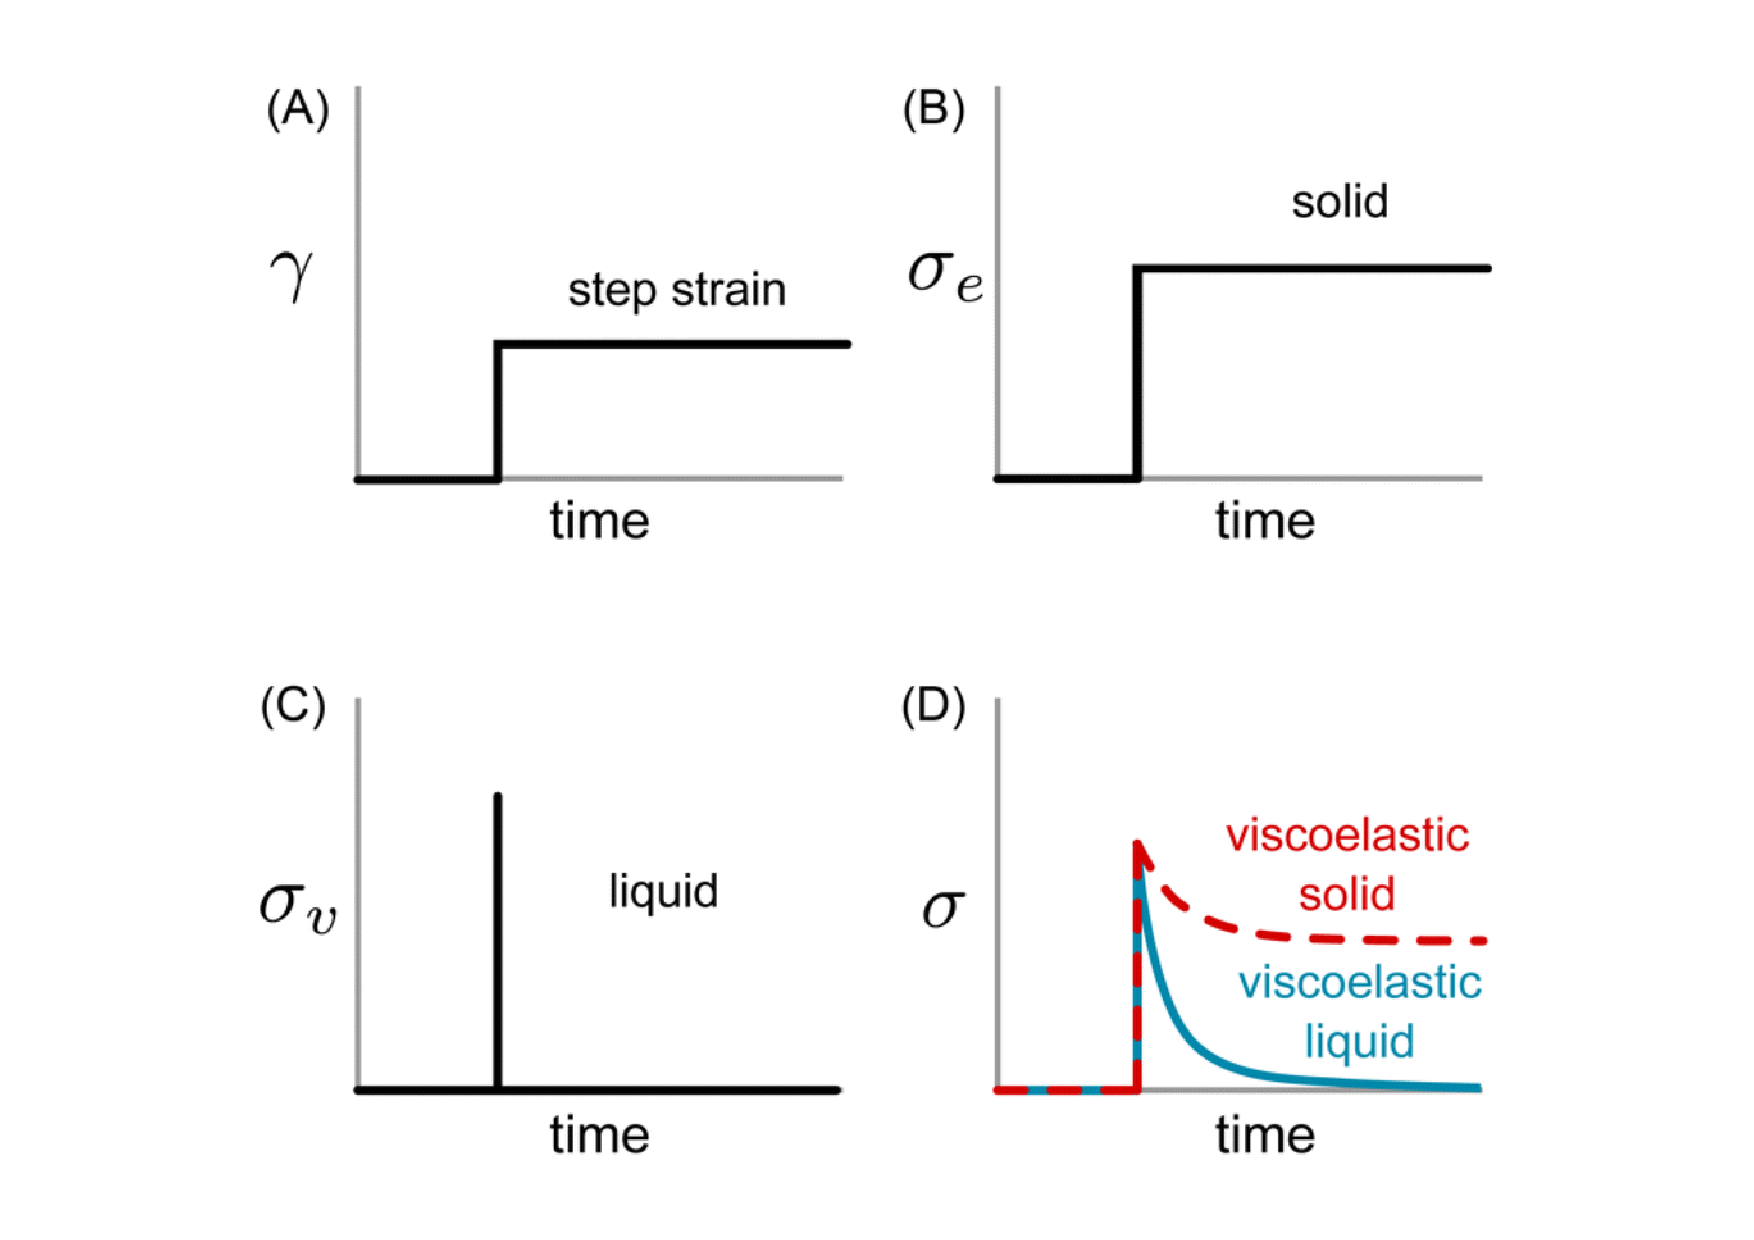
\includegraphics[width=\textwidth]{Fig/solid_liquid.pdf}
	\FigureBicaption{\label{differ_fluid_intro}(A)施加的应变曲线以及对应的剪切应力(B)理想弹性固体(C)理想粘性液体(D)粘弹性样品\cite{ricarteTutorialReviewLinear2024}}{(A) Applied strain profile and resulting shear stress (B) Ideal elastic solid (C)Ideal viscous liquid (D) Viscoelastic samples\cite{ricarteTutorialReviewLinear2024}}
\end{figure}
图\ref{differ_fluid_intro}概述了两种不同类型的粘弹性材料的简单剪切行为。对于粘弹性固体和液体,阶跃应变会引起瞬时弹性响应,从而产生$\sigma$峰值。然而,应力不是保持不变或立即降至零,而是逐渐降低。它在很长一段时间内接近粘弹性固体的有限平台值,而粘弹性液体则完全衰减到零\cite{ricarteTutorialReviewLinear2024}。

线性本构理论中最经典的是Maxwell模型\cite{maxwell1867iv},如图\ref{maxwell_intro}所示,Maxwell模型将材料的弹性行为和粘性行为结合起来,它用一个弹簧(弹性元件)和一个粘壶(粘性元件)串联表示黏弹性关系。Maxwell模型的微分形式如公式\eqref{eq:maxwell_model_dt}所示,其中$\tau$表示松弛时间,等于$eta/G$。将两边积分得到Maxwell模型的积分形式如公式\eqref{eq:maxwell_model_int}所示。
\begin{align}
	 & \frac{d\sigma}{dt} + \frac{\sigma}{\tau}  = G \frac{d\gamma}{dt} \label{eq:maxwell_model_dt}                                                   \\
	 & \sigma(t)                                = \int_{-\infty}^{t} G e^{-\frac{t-t'}{\tau}} \frac{d\gamma(t')}{dt'} dt'\label{eq:maxwell_model_int}
\end{align}
积分形式的方程显示了任何时刻的应力是松弛模量乘以应变速率的积分,该时刻之前材料的整个历史。由于被积函数中的衰减指数,模型具有衰落的记忆,因此最近的应变历史比过去的应变历史更重要。
\begin{figure}[htbp]
	\centering
	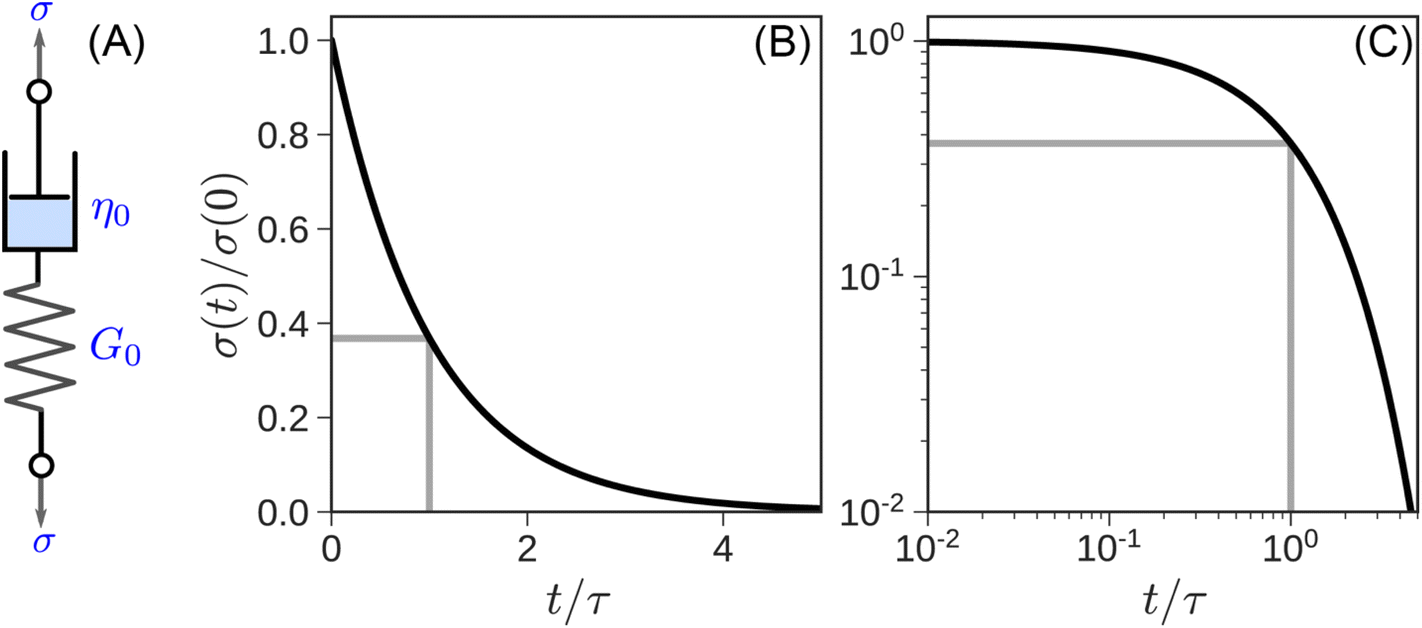
\includegraphics[width=0.8\textwidth]{Fig/maxwell_intro.png}
	\FigureBicaption{\label{maxwell_intro} Maxwell 模型示意图}{Schematic illustration of Maxwell model}
\end{figure}
如果将多个Maxwell模型并联,便可以得到广义Maxwell模型方程,如公式\eqref{eq:generalized_maxwell_model}所示。
\begin{equation}
	\sigma(t) = \int_{-\infty}^{t} G(t-t') \frac{d\gamma(t')}{dt'} dt' \label{eq:generalized_maxwell_model}
\end{equation}
其中松弛模量 \(G(t)\) 定义为公式\eqref{eq:generalized_maxwell_model_G}。
\begin{equation}
	G(t) = \sum_{i=1}^{n} G_i e^{-\frac{t}{\tau_i}} \label{eq:generalized_maxwell_model_G}
\end{equation}

Maxwell模型通过将黏弹性抽象为黏性元件和弹性元件串联来得到本构方程。如果将弹簧和粘壶进行并联,则得到Kelvin-Voigt模型的本构方程,即公式\eqref{eq:kelvin_voigt_model}\cite{voigt1892ueber}。
\begin{equation}
	\sigma(t) = G \gamma(t) + \eta \frac{d\gamma(t)}{dt} \label{eq:kelvin_voigt_model}
\end{equation}
将多个Kelvin-Voigt模型的元件进行串联,便可以得到广义Kelvin-Voigt模型,如公式\eqref{eq:generalized_kelvin_voigt_model}。
\begin{equation}
	\sigma(t) = \sum_{i=1}^{n} \left( G_i \gamma_i(t) + \eta_i \frac{d\gamma_i(t)}{dt} \right)\label{eq:generalized_kelvin_voigt_model}
\end{equation}
原则上,任何广义Voigt模型都可以在数值上映射到等效的广义 Maxwell模型,这是线性本构方程构建的基本研究方法的不同角度\cite{ricarteTutorialReviewLinear2024}。

如果将传统的整数阶导数模型改为分数阶导数,能够更加准确描述材料的记忆效应。例如Bagley和Torvik等在20世纪80年代提出的分数阶Maxwell模型,是对传统Maxwell模型的推广\cite{bagley1986fractional}。无论是什么形式的线性本构方程,均满足一个基本假设材料的响应是线性的,即多个应变历史的叠加效应等于各自效应的线性相加,当公式\eqref{eq:generalized_maxwell_model}中的松弛模量G表示为公式\eqref{eq:generalized_maxwell_model_G}时是Maxwell模型的形式,事实上当G为一个抽象的松弛函数时,公式\eqref{eq:generalized_maxwell_model}抽象为更一般的线性本构方程,被称为玻尔兹曼叠加原理(BSP),玻尔兹曼叠加原理广泛应用于描述线性黏弹性材料的行为,例如应力松弛、蠕变、动态力学响应等\cite{boltzmannZurTheorieElastischen1878}。
\subsection{非线性本构方程}
线性本构方程只能用于描述只能描述简单的材料行为,例如弹性变形、小应变下的黏弹性行为\cite{fedorowiczElasticPerfectlyPlastic2024,lingComparisonReviewClassical2023,ricarteTutorialReviewLinear2024}。适用于材料在小变形范围内的线性响应。能够描述复杂的材料行为,而非线性本构方程可以用来描述更为复杂的行为例如塑性变形、硬化或软化、各向异性、大变形、剪切稀化、剪切增稠等行为。绝大部分高分子材料具有较复杂的非线性关系。Binham提出模型认为屈服性流体当剪应力低于屈服应力时,流体表现为刚性固体;当剪应力超过屈服应力时,流体开始流动,且流动行为类似于牛顿流体\cite{binghaminvestigation}。Herschel-Bulkley模型在此基础之上引入了剪切稀化和剪切增稠的表示,如公式\eqref{eq:herschel},是描述非线性本构方程的一套公式\cite{herschel1926konsistenzmessungen}。
\begin{equation}
	\sigma=\sigma_0+K\dot{\gamma}^n \label{eq:herschel}
\end{equation}
松弛模量函数不仅是时间的函数,也是应变的函数,能够表征大变形下的非线性响应。改进的Herschel-Bulkley类模型在Herschel-Bulkley模型的基础上,通过引入额外的参数或修正项,显著提升了对流体行为的描述精度。例如,在Herschel-Bulkley模型中引入高阶项(如剪切速率的二阶项),可以更准确地刻画非线性流变行为\cite{magnon2021precise}。此外,通过引入Papanastasiou正则化方法,有效解决了原始模型在低剪切速率下的数值不稳定性问题,这一改进模型被称为Herschel-Bulkley-Papanastasiou (HBP) 模型。HBP模型在磁流变液等复杂流体的流变特性描述中得到了广泛应用\cite{papanastasiou1987flows}。
Herschel-Bulkley类模型不涉及弹性流体,主要用于解决屈服应力流体的本构问题,对于黏弹性流体的非线性本构方程而言,可以写出一般的通式,如公式\eqref{eq:nolinear_model},非线性黏弹性流体的本构方程可以从宏观连续介质力学和微观分子角度分别进行描述\cite{ewoldtDesigningComplexFluids2022}。
\begin{equation}
	\sigma(t) = \int_{-\infty}^{t} G(t-t',\gamma) \frac{d\gamma(t')}{dt'} dt' \label{eq:nolinear_model}
\end{equation}

宏观介质力学中Oldroyd-B模型,如公式\eqref{eq:oldroyd_b}是在Maxwell模型的基础上作了修正,增加了延迟时间项$\lambda_2$ ,从而能够描述更复杂的流变行为,同时这个模型引入了上随体导数来代替普通导数,在物理上更加符合真实世界的材料行为。Oldroyd-B模型本意可以在Weissenberg数($W_i=\lambda_1 \dot{\gamma}_i$)较小的情况下描述线性黏弹性,但是其中的上随体导数在一定程度上包含了部分非线性效应,特别是在高应变率或大变形条件下。Oldroyd-B模型是非线性本构方程的经典基础模型,研究者在此基础上为了更准确地描述非线性黏弹性行为,研究者提出了多种修正的 Oldroyd-B模型。
\begin{equation}
	\boldsymbol{\sigma} + \lambda_1 \frac{\mathcal{D}\boldsymbol{\sigma}}{\mathcal{D}t} = \eta \left( \dot{\boldsymbol{\gamma}} + \lambda_2 \frac{\mathcal{D}\dot{\boldsymbol{\gamma}}}{\mathcal{D}t} \right) \label{eq:oldroyd_b}
\end{equation}
Giesekus模型(公式\eqref{eq:giesekus})在Oldryd-B模型基础上,增加了一个非线性项,通过非线性系数$\alpha$来表示非线性行为。Giesekus模型常用于描述高聚物溶液、熔体以及其他粘弹性流体的流变行为。这些流体通常表现出剪切稀化和弹性效应。尤其是在中等至高剪切速率范围内。其模型参数(如迁移因子α)可以调节剪切稀化的强度和拐点形状,具有较高的灵活性。Giesekus模型在高Weissenberg数(Wi)条件下仍能保持数值稳定性,适用于强弹性效应的流动场景。通过引入对数构象重构等方法,可以进一步提高其在高Wi条件下的计算稳定性。
\begin{equation}
	\boldsymbol{\sigma} + \lambda_1 \frac{\mathcal{D}\boldsymbol{\sigma}}{\mathcal{D}t} + \alpha \frac{\lambda_1}{\eta} \boldsymbol{\sigma} \cdot \boldsymbol{\sigma} = \eta \left( \dot{\boldsymbol{\gamma}} + \lambda_2 \frac{\mathcal{D}\dot{\boldsymbol{\gamma}}}{\mathcal{D}t} \right) \label{eq:giesekus}
\end{equation}
PTT模型(公式\eqref{eq:ptt})通过引入一个非线性应力函数$f$扩展了Oldroyd-B模型。该函数通常取指数形式。
\begin{equation}
	f(\text{tr}(\boldsymbol{\sigma})) \boldsymbol{\sigma} + \lambda_1 \frac{\mathcal{D}\boldsymbol{\sigma}}{\mathcal{D}t} = \eta \left( \dot{\boldsymbol{\gamma}} + \lambda_2 \frac{\mathcal{D}\dot{\boldsymbol{\gamma}}}{\mathcal{D}t} \right) \label{eq:ptt}
\end{equation}
FENE-P模型(公式\eqref{eq:fene_p})在 Oldroyd-B 模型的基础上引入了有限拉伸效应,通过项$\frac{\lambda_1}{\eta} \frac{\boldsymbol{\sigma}}{1 - \text{tr}(\boldsymbol{\sigma})/b}$描述聚合物链的有限拉伸行为。参数$b$表示聚合物链的最大拉伸比。该模型适用于描述聚合物溶液在强流动条件下的非线性行为。
\begin{equation}
	\boldsymbol{\sigma} + \lambda_1 \frac{\mathcal{D}\boldsymbol{\sigma}}{\mathcal{D}t} = \eta \left( \dot{\boldsymbol{\gamma}} + \lambda_2 \frac{\mathcal{D}\dot{\boldsymbol{\gamma}}}{\mathcal{D}t} \right) - \frac{\lambda_1}{\eta} \frac{\boldsymbol{\sigma}}{1 - \text{tr}(\boldsymbol{\sigma})/b} \label{eq:fene_p}
\end{equation}
通过将Oldroyd-B模型与分数阶导数结合,可以得到分数阶Oldroyd-B模型,如公式\eqref{eq:fractional_oldroyd_b}。分数阶 Oldroyd-B模型通过引入分数阶导数描述非局部记忆效应。参数$\alpha$和$\beta$是分数阶导数的阶数,该模型能够捕捉更复杂的流变行为,适用于具有非局部记忆效应的复杂流体。
\begin{equation}
	\boldsymbol{\sigma} + \lambda_1^\alpha \frac{\mathcal{D}^\alpha \boldsymbol{\sigma}}{\mathcal{D}t^\alpha} = \eta \left( \dot{\boldsymbol{\gamma}} + \lambda_2^\beta \frac{\mathcal{D}^\beta \dot{\boldsymbol{\gamma}}}{\mathcal{D}t^\beta} \right) \label{eq:fractional_oldroyd_b}
\end{equation}
Oldroyd-B类本构模型均为微分型本构模型,源于微分型Maxwell模型公式\eqref{eq:maxwell_model_dt}。另一类本构模型如K-BKZ模型源于积分型Maxwell模型公式\eqref{eq:maxwell_model_int}。
K-BKZ模型如公式\eqref{eq:k_bkz_model}所示。在 K-BKZ 模型中,$h$ 称为阻尼函数,它是形变张量的第一不变量 $I_1$ 和第二不变量 $I_2$ 的函数。$\mathbf{C}^{-1}(t,t')$ 是Finger 形变张量的逆,用于描述从时间 $t'$ 到 $t$ 的形变历史。$m(t-t')$ 是瞬态函数或记忆函数,用于表征材料对历史形变的记忆效应。K-BKZ 模型广泛应用于聚合物加工(如挤出、注塑、热成型等)、生物流体力学(如血液、蛋白质悬浮液等复杂流体的流变行为研究)以及涂料和润滑剂的流动行为和流变特性分析\cite{mitsoulis60YearsKayeBernstein2023}。
\begin{align}
	% K-BKZ 模型基本形式
	 & \boldsymbol{\sigma}(t)  = \int_{-\infty}^t m(t-t') \, h(I_1, I_2) \, \mathbf{C}^{-1}(t,t') \, dt'    \label{eq:k_bkz_model}
\end{align}

Doi和Edwards尝试从分子角度构建本构方程,在管子模型的基础上提出了Doi-Edwards模型(公式\eqref{eq:doi_edwards})。Doi-Edwards 模型的核心思想是将高分子链的缠结效应简化为一条光滑管道对链的限制作用,链在管道中的运动通过松弛和扩散来描述。其中$G_0$表示松弛时间,而$Q$表示为公式\eqref{eq:doi_edwards_q},反映了高分子链在形变历史下的方向分布变化,即链的取向如何随形变而变化。
\begin{align}
	 & \boldsymbol{\sigma}(t)  = G_0 \int_{-\infty}^t \frac{\partial Q(\mathbf{E}(t,t'))}{\partial t'} \, dt'    \label{eq:doi_edwards}                                                                  \\
	 & Q(\mathbf{E}(t,t'))     = \frac{5}{2} \left\langle \frac{\mathbf{E}(t,t') \cdot \mathbf{u} \mathbf{u}}{|\mathbf{E}(t,t') \cdot \mathbf{u}|^2} \right\rangle_{\mathbf{u}} \label{eq:doi_edwards_q}
\end{align}
传统的 Doi-Edwards模型基于单链平均场近似,将缠结效应简化为一条光滑的“管子”对高分子链的限制作用。然而,这种简化忽略了链-链间的直接相互作用,难以解释快速大形变条件下的非线性流变现象(如应力过冲、缠结点破损和重组等)。近年来,研究者通过引入多链相互作用,提出了修正的管子模型,例如 GLaMM 理论,在此基础之上能够更好地描述缠结高分子流体的非线性行为。

\subsection{传统的本构方程的构建方法}
传统本构方程尤其是Oldroyd-B、Doi-Edwards等复杂的非线性模型具有较多的待定参数,通过数学形式描述材料的应力-应变关系及其对时间、温度和形变历史的依赖性。其构建方法主要基于实验观测、理论推导和数值模拟的结合,通常分为以下几个步骤。

首先,实验观测是构建本构方程的基础。通过流变学实验(如剪切流变、拉伸流变等),研究者可以获取材料在不同形变条件下的应力响应数据。这些实验数据为理论模型的构建提供了关键依据。例如,通过动态力学分析(DMA)测量材料的存储模量和损耗模量,可以确定其粘弹性特性;通过应力松弛和蠕变实验,可以推断材料的记忆效应和时间依赖性。实验数据的精确性和全面性直接决定了本构方程的适用性和预测能力。

其次,理论推导是本构方程构建的核心环节。对于线性粘弹性材料,通常采用弹簧和粘壶的组合模型(如Maxwell模型、Kelvin-Voigt模型)来描述其力学行为,通过不同的组合可以表示不同的本构方程。对于非线性材料,则需要引入更复杂的本构关系,这里主要还是基于线性黏弹性方程,通过各类引入非线性关系的方法来进行非线性关系推导,理论推导的关键在于如何将微观结构信息(如高分子链的缠结、颗粒的相互作用等)与宏观力学行为联系起来。而对于理论推导的结果,每一个非线性项或参数应当从数学角度进行证明。例如近年来,数学研究者对Doi-Edwards模型的适定性进行了深入研究。Chupin等人通过Schauder不动点定理和Galerkin近似方法,证明Doi-Edwards 模型在二维情况下的全局解存在性和唯一性。这一结果为模型的数学基础提供了严格的理论支持。

数值模拟在本构方程的构建和验证中发挥着关键作用。有限元分析(FEA)、有限差分法(FDM)和有限体积法(FVM)等数值方法能够将本构方程应用于复杂几何和边界条件下的力学问题,从而模拟材料的应力分布、形变行为和流动特性。例如,在聚合物加工领域,研究者通过结合有限元分析和Doi-Edwards模型,能够预测熔体在挤出或注塑过程中的流动行为,并优化加工参数。分子动力学模拟(MD)是另一种重要的数值工具,能够从分子尺度模拟材料的力学行为,为宏观本构方程的构建提供微观依据。例如,通过粗粒度分子动力学模拟(CGMD),研究者可以研究高分子链的缠结动力学,验证管子模型的假设。由于聚合物液体具有单体、中观和宏观流尺度的多尺度特征,因此关联不同层次的多尺度模拟(MSS)能够更准确地再现其流动特性。
\begin{figure}[htbp]
	\centering
	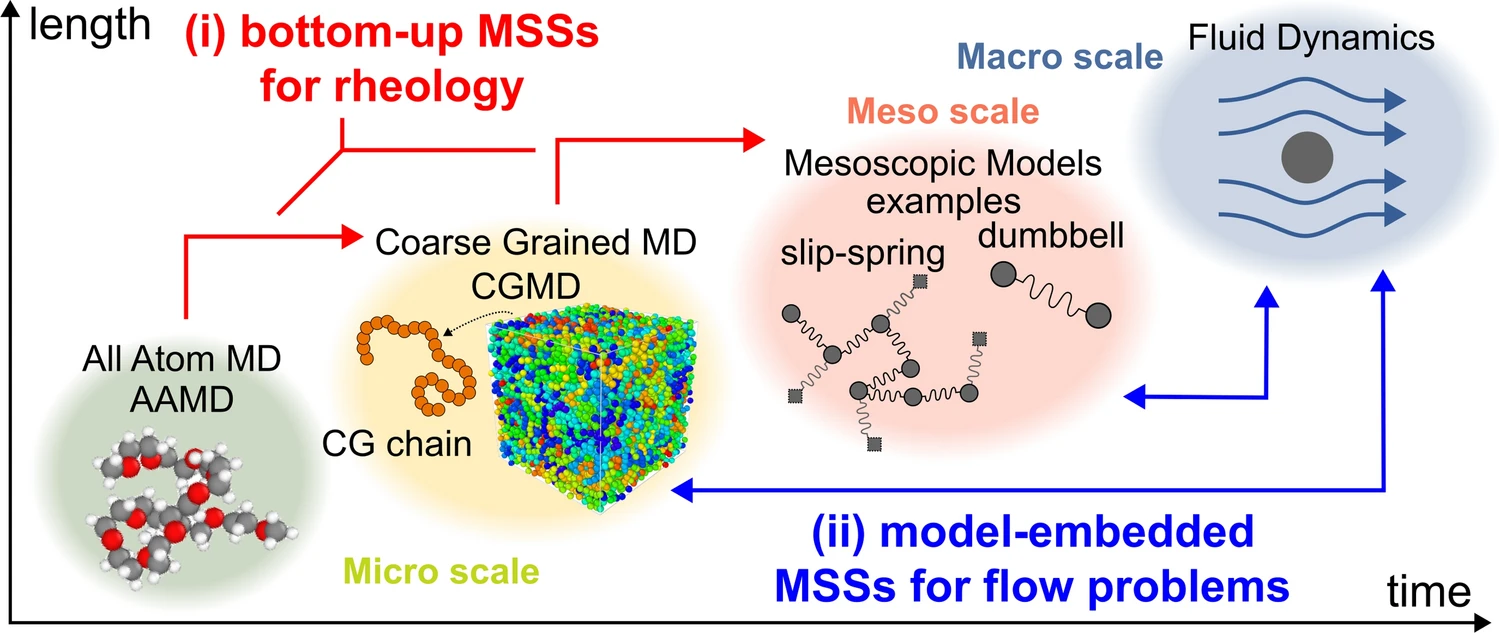
\includegraphics[width=0.8\textwidth]{Fig/duochidumoni.png}
	\FigureBicaption{\label{duochidumoni} 多尺度模拟示意图}{Schematic illustration of Multiscale Simulation}
\end{figure}

传统本构方程的研究方法主要依赖于物理实验和理论推导,通过建立数学方程来描述材料的力学行为。这种方法虽然具有明确的物理意义,但在处理复杂材料或非线性行为时,往往面临模型精度不足、参数识别困难等问题。随着数据驱动技术的快速发展,机器学习为材料本构关系的研究提供了新的思路。通过利用大量实验或仿真数据,机器学习能够自动挖掘材料行为中的潜在规律,构建高精度的预测模型,从而弥补传统方法的不足,并为材料科学的研究开辟了更加智能化的路径。
\section{机器学习应用于流变学本构关系研究现状}
\subsection{机器学习方法介绍}
机器学习是人工智能的一个重要分支,其核心是通过算法从数据中自动学习规律,并利用这些规律进行预测或决策。与传统编程不同,机器学习不依赖于明确的规则,而是通过训练数据优化模型参数,从而实现对复杂问题的建模和解决。它在图像识别、自然语言处理、推荐系统等领域取得了显著成果。

监督学习是最常见的机器学习类型,适用于有标签的数据集。常见的算法包括线性回归和逻辑回归,分别用于连续值的预测和二分类问题。决策树(DT)通过树状结构进行决策,适用于分类和回归任务。随机森林(RF)是多个决策树的集成,通过投票或平均提高预测准确性。支持向量机(SVM)通过寻找最优超平面进行分类,适用于高维数据。K近邻算法(KNN)基于距离度量进行分类或回归,简单但计算量大。朴素贝叶斯算法基于贝叶斯定理,适用于文本分类等任务。无监督学习则更多处理无标签数据,主要用于数据聚类和降维。

随着数据规模和计算能力的提升,深度学习作为机器学习的一个子领域迅速崛起。深度学习通过构建多层的神经网络结构,能够自动提取数据中的多层次特征,从而在处理高维、非线性问题(如图像、语音和文本)时表现出更强的能力,成为推动人工智能发展的核心技术之一。

近年来,深度学习领域不断涌现出新的理论和应用,进一步拓展了机器学习的边界。扩散模型通过模拟数据从噪声到清晰图像的逆扩散过程,逐步生成高质量的图像,在图像生成、风格迁移和图像修复等任务中表现出色。多模态学习则通过同时处理文本、图像、音频和视频等多种数据类型,实现了更全面的内容理解和生成,例如CLIP模型通过学习图像和文本的关联,实现了零样本分类和图像搜索任务。自监督学习通过利用数据本身的结构生成标签,减少了对人工标注数据的依赖,对比学习通过最大化相似样本的表示一致性,显著提升了模型的特征提取能力。这些前沿进展不仅推动了深度学习技术的发展,也为解决实际问题提供了新的思路和方法,未来将在更多领域展现出强大的潜力。

\subsection{纯数据驱动的机器学习研究现状}
\subsubsection{引言}
传统机器学习或是目前最前沿的深度学习研究,最初都集中于计算机科学、人工智能领域,但是近年来在物理学领域,机器学习与物理学问题的研究结合也日益密切。在量子物理中,机器学习被用于量子态重构、量子电路优化和量子相变识别,显著提高了量子系统的分析和计算效率。在凝聚态物理领域,机器学习通过预测材料性质和分类相图,加速了新材料的发现和设计。在天体物理中,机器学习被用于引力波探测和宇宙微波背景辐射分析,揭示了宇宙的起源和结构。在流体动力学中,机器学习通过数据驱动的方法直接从流体数据中学习湍流动力学,显著提高了湍流模型的精度和计算效率。此外,机器学习中的符号回归技术能够从实验数据中自动发现物理定律,为探索未知物理规律提供了新工具;在多尺度物理系统中,机器学习被用于气候模拟和生物信息学建模,预测复杂动态和处理多重空间和时间尺度的混沌系统。

在流变学领域,机器学习也被广泛应用。传统的流变学研究方法如上一章所述,通过获取数据,通过数学物理方程解释数据。传统的流变学家总是期待于对每个流变学体系建立一个可表示的数学方程,尽管这个方程可能完全无法求出解析解也极难获取稳定精确的数值解。这本质上是一个由因推果的过程,而数据驱动的机器学习方法则从真实的结果出发,构建一个完全匹配的数学方程,这个方程的形式与参数都不确定,但是可以泛化本构现象,即通过含有大量参数的非方程化的计算机模型代替具体形式的本构方程来解决流变学本构问题。
\begin{figure}[htbp]
	\centering
	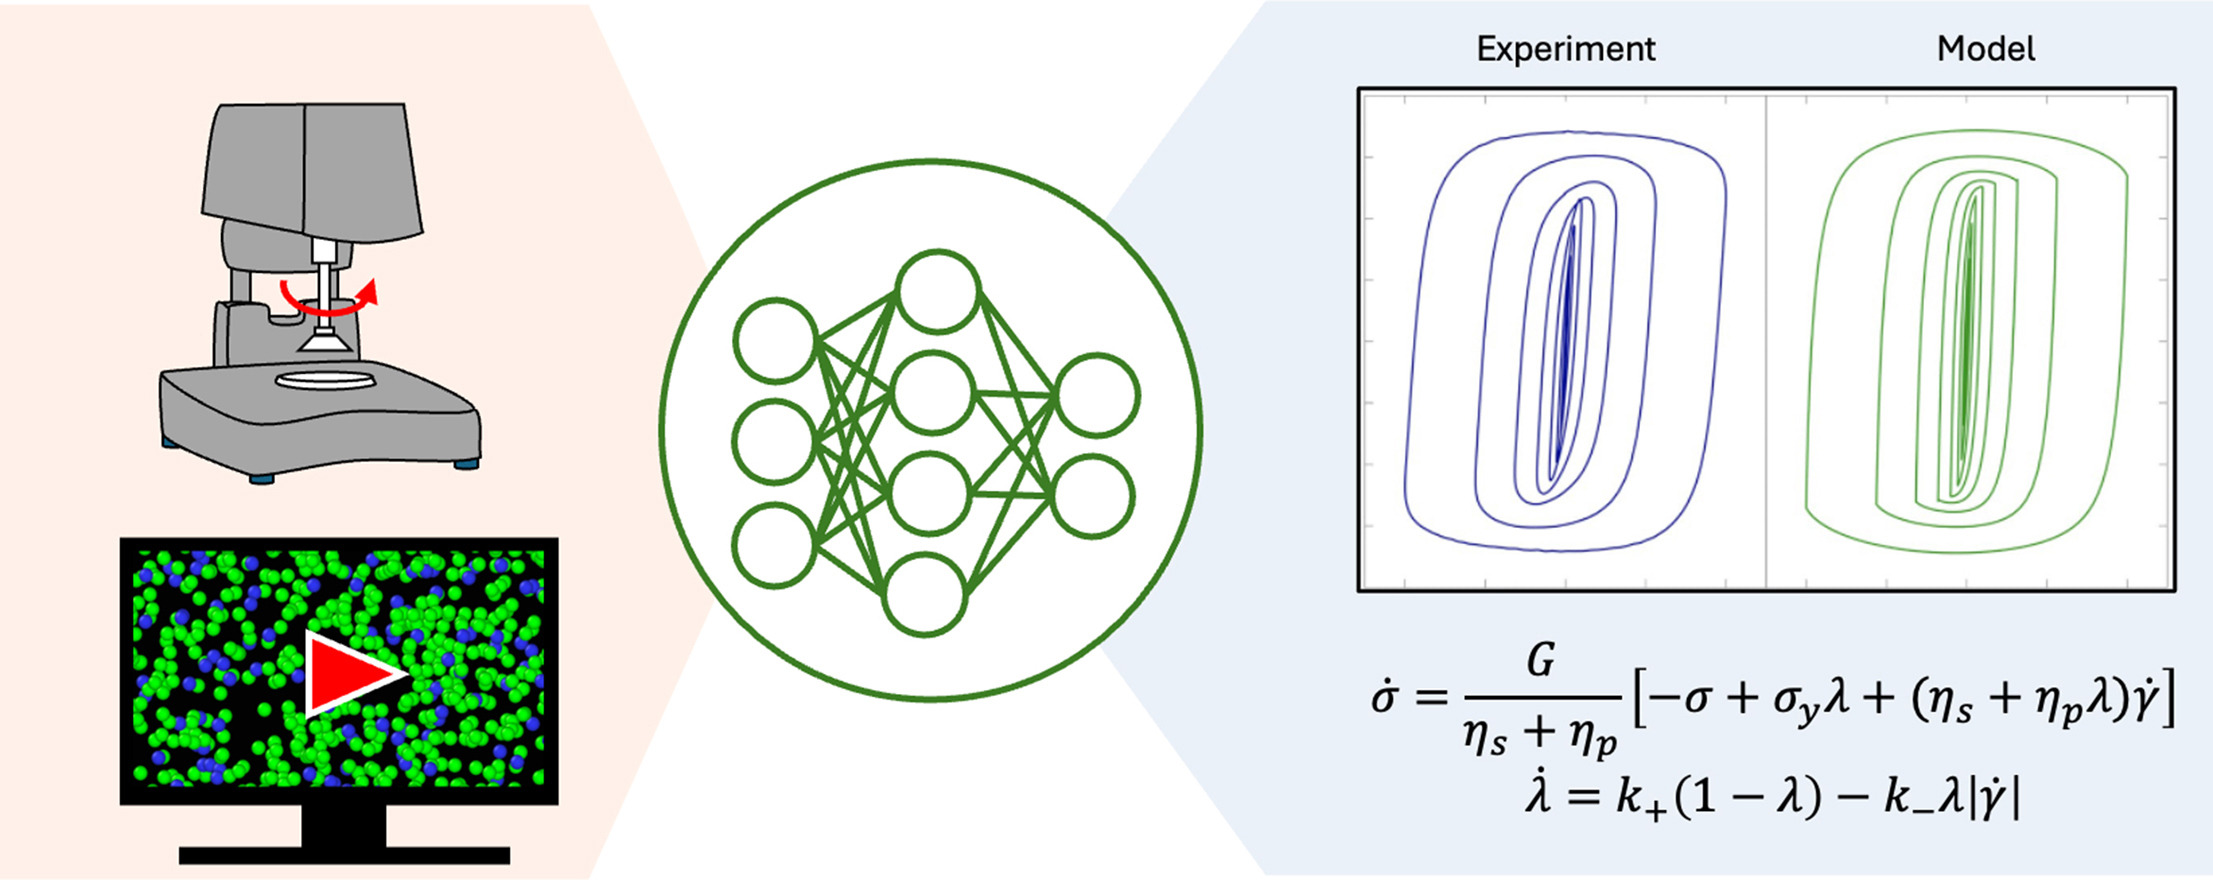
\includegraphics[width=0.8\textwidth]{Fig/datadrivenintro.jpg}
	\FigureBicaption{\label{datadrivenintro} 数据驱动方法应用于流变学研究示意图}{Schematic illustration of data-driven methods applied to rheology research}
\end{figure}

\subsubsection{流变特性预测}
机器学习应用于流变学本构的其中一个应用是流变特性的预测。人工神经网络(ANN)已被用于自动监测合成油基泥浆的各种流变特性,使用泥浆密度和沼泽漏斗作为输入,预测值与实际测量值非常接近,平均绝对误差小于 9.66\%。混合机器学习模型结合了ANN和SVM准确预测了纳米基水基钻井液的流变性和过滤特性。四种不同的模型——多元线性回归(MLR)、SVM、回归决策树(CART)和ANN被一起使用,以根据溶液特性预测聚合物溶液的粘度,有助于提高石油采收率。此外,机器学习模型可以与微流体或其他设备集成,用于复杂流体的原位粘度测量。例如,Mustafa等设计了一种微流体传感设备,利用流固耦合和ML算法来测量复杂流体的粘度。他们采用SVM和KNN算法,分别实现了89.7\%和98.9\%的平均准确率。Ponick等利用卷积神经网络(CNN)通过立体相机图像预测Bingham流体的流变特性。Chen等人通过将群贡献 (GC) 方法与著名的机器学习算法,即人工神经网络 (ANN) 相结合,以预测离子液体 (IL) -水混合物的粘度。张等人开发了一种深度半监督的基于即时学习的高斯过程回归 (DSSJITGPR) 用于门尼粘度估计。它将即时学习、半监督学习和深度学习集成到一个统一的建模框架中。DSSJITGPR的有效性和优越性已通过工业橡胶混炼过程的Mooney粘度预测结果得到验证。

\subsubsection{材料表征和工艺设计优化}
机器学习在流变学本构中的应用不仅限于材料表征和工艺设计/优化,还通过直接引入材料制备和表征中的各种参数作为特征,显著简化了传统本构方程中针对特定材料体系拟合不同参数的复杂性。与传统统计方法相比,机器学习算法能够更高效地对这些复杂关系进行建模,其中主成分分析和深度神经网络等技术在管理和减少材料表征中常见的高维数据方面发挥了重要作用,从而实现了更高效的分析和解释。这些方法已广泛应用于3D打印混凝土、纤维增强混凝土、聚合物纳米复合材料、生物墨水、食品材料和高分子科学等领域。Zhang和Shao的研究进一步探讨了基于图像的机器学习技术在材料科学中的应用,以应对各种挑战和任务,由于这些方法的通用性和可转移性,它们同样适用于流变学表征。机器学习模型还彻底改变了高通量表征,为数据分析、预测和优化提供了强大的工具。例如,Zhang等人开发了一种自主高通量系统,采用支持向量机(SVM)、随机森林(RF)和极端梯度提升(XGB)分类器等监督式机器学习算法,快速表征水凝胶的流变特性,所有模型在水凝胶相分类中均表现出色。Verheyen等人则利用基于树的集成算法(如随机森林和梯度提升)将数据驱动建模与颗粒水凝胶基质系统的实验优化相结合,这些技术因其在处理分类或回归任务、非线性关系、高维数据和混合数据类型方面的灵活性而被选用。Martineau等人开发了一种基于高斯过程(GP)建模的管道,用于识别细菌嵌入的丝水凝胶的凝胶化状态,通过比较人类专家和机器学习引导算法的性能,发现两者结合最能加速发现过程。此外,随机森林和多元线性回归(MLR)等技术已被用作回归工具,将从大振幅振荡剪切(LAOS)实验中获得的流变特性与人类感官感知(如涂抹性)相关联,从而改进化妆品行业的配方设计。Lee等人的研究表明,由于流变测量和铺展性之间的非线性关系,随机森林模型的性能优于多元线性回归模型

\subsubsection{助力流变学计算模拟}
机器学习为流变学的计算模拟提供助力,计算平台已经成为流变学研究的重要支柱,广泛应用于从聚合物动力学到颗粒系统的详细模拟,为复杂流体在不同条件下的行为提供了深刻的物理见解。然而,这些技术的主要瓶颈在于模拟与实验条件相关的时间和长度尺度的能力。由于大规模模拟中的大部分计算资源消耗在重复的数学运算上,而这些运算可以通过数据驱动技术高效学习,因此将机器学习与模拟相结合能够显著提升效率和精度。例如,Lu等人基于卷积神经网络的仿真模型在颗粒流模拟中实现了显著的加速,同时保持了较高的精度;高斯过程回归则被Seryo等人用于从微观聚合物模拟中推断本构关系,并将这些关系应用于宏观流动仿真,从而调整流体中的应力分布以反映微观动力学。类似的方法还被应用于缠结良好的聚合物熔体,通过机器学习的本构关系优化模拟效果。此外,Bai等人介绍了一种数据驱动的平滑粒子流体动力学方法,该方法利用实验数据提高了牛顿流体和非牛顿流体的建模精度,即使在数据集较小的情况下也能准确预测幂律流体的速度曲线,同时显著优化计算时间。多尺度建模通过在不同尺度之间交换信息来捕捉材料的复杂行为,例如Li等人基于生成对抗网络的方法实现了从粗粒度到原子级别的结构回溯映射。主动学习作为一种高效的机器学习范式,通过选择性地标记信息量最大的数据点,以最少的数据优化学习过程,例如在多尺度建模中,Zhao等人基于高斯过程回归的主动学习策略将所需的模拟次数大幅减少,显著提高了研究复杂材料行为的效率。这些技术的结合不仅提升了模拟的精度和效率,还为流变学研究提供了更强大的工具。

\subsubsection{小结}
以数据为中心的机器学习模型严重依赖丰富的训练数据来确保预测的可靠性和准确性,无论其架构或算法如何设计。此外,材料特性通常对成分和加工条件的细微变化表现出高度敏感性,这可能导致材料行为的显著变化。因此,数据收集过程必须足够全面和细致,以捕捉这种复杂性,从而确保以数据为中心的模型能够做出准确的预测。例如,对于具有整体Herschel-Bulkley类型行为的屈服应力流体,如果算法仅暴露在大变形率或小变形率下的数据中,它将无法对观察域之外的一般行为做出可靠预测。更重要的是,这些模型完全依赖于数据相关性和统计规律,而忽略了基础科学理论的支持,例如黏弹性材料的时间依赖性和应变依赖性等关键物理特性。纯数据驱动方法往往忽视了这些物理细节,导致模型在实际应用中可能失效。因此,在开发算法时,我们应当引入物理约束,将黏弹性的时间依赖性等基本物理规律纳入模型框架,以弥补数据驱动方法的不足,从而提升模型的预测能力和泛化性能。
\subsection{引入物理约束的神经网络研究}
\subsubsection{引言}
近年来,多种方法被提出并广泛应用于将基本物理规则和领域知识整合到机器学习框架中,这些方法在众多领域展现了深远的影响。这类模型的总体框架通常被称为物理信息机器学习(PIML)。PIML的一个开创性范例是“物理信息神经网络”(PINN),它代表了科学计算和应用数学领域的重大突破。PINN将机器学习算法与从系统观察、经验以及物理或数学理解中获得的先验知识无缝结合,通过将这些先验知识直接嵌入模型架构中,显著减少了对大规模训练数据集的依赖,从而能够利用更少的观测数据解决复杂的物理问题。

\subsubsection{物理信息神经网络研究现状}
近年来,物理信息神经网络(PINN)在流变学建模领域取得了重要进展,有效克服了传统方法依赖简化假设和难以处理复杂材料特性的局限。Mahmoudabadbozchelou等人提出的流变学信息神经网络(RhINN)框架,能够处理触变性弹性粘塑性(TEVP)模型等多种本构模型。该框架以时间t和剪切速率为输入,剪应力$\sigma$和结构参数$\lambda$为输出,通过最小化包含方程残差和初始条件差异的损失函数来训练网络参数。在逆问题求解中,RhINN可同时学习网络参数和流变参数,其预测结果与真实数据高度吻合,展现了良好的鲁棒性。Dabiri等人进一步将RhINN扩展至分数阶微分方程,提升了其在复杂本构模型参数识别中的应用价值。在相关研究中,Zhang等人开发的RheologyNet成功应用于胶凝材料触变特性评估,其预测结果与有限元分析高度一致。Nagrani等人则利用PINN研究了导热硅脂的流变行为,通过实验数据确定了流变参数。基于物理的机器学习方法还可从间接观测中学习未知流变模型,例如通过三维流场数据推断广义牛顿流体的稳态剪切粘度,这一方法在聚合物熔体和颗粒悬浮液研究中取得了显著成果。此外,PINN在稀薄气体流动预测中也展现出应用潜力。Howard等人将悬浮平衡模型与神经网络结合,成功预测了单分散悬浮液的颗粒应力,但在双分散系统中的应用仍存在局限。这些研究充分展示了物理信息神经网络在流变学领域的广泛应用前景。
\begin{figure}[htbp]
	\centering
	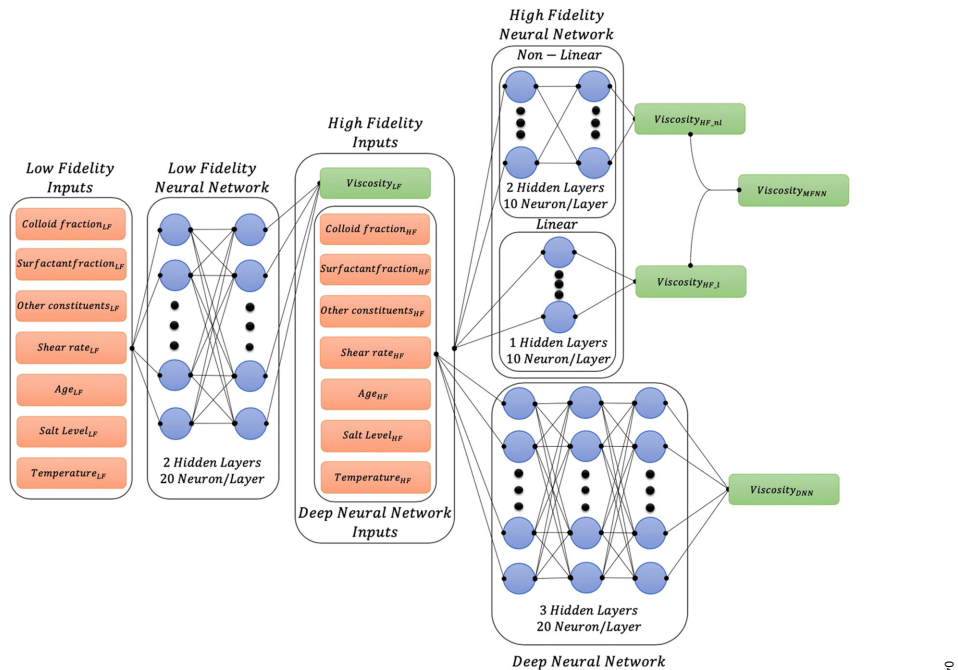
\includegraphics[width=0.8\textwidth]{Fig/MFNN.png}
	\FigureBicaption{\label{mdnn} 多保真神经网络(MFNN)结构示意图}{ Schematic illustration of Multifidelity Neural Network (MFNN) structure}
\end{figure}

多保真度建模是一种强大的技术,通过整合来自不同保真度和计算成本的数据来增强模型预测能力。这种方法在物理定律不精确或高保真数据生成成本较高的情况下尤为有用。通过高效结合高保真和低保真数据,多保真度建模为复杂系统的精确建模提供了一种更高效且更具成本效益的解决方案。例如,Mahmoudabadbozchelou等人利用多保真度方法构建了一个流变学元模型,用于预测复杂多组分系统的流变响应,同时考虑了老化、混合物的盐度和温度依赖性等输入参数。在该框架中,低保真数据通过多种本构方程生成,而高保真数据则来自实验测量。与传统的高保真神经网络相比,这种组合方法显著提高了预测精度,充分展示了多保真度建模的优势。

类似的方法也被应用于预测纤维悬浮液的流变特性,其中基于法向载荷相关摩擦系数模型的数值模拟用于生成高保真数据,而低保真数据则通过不同的本构模型生成。纤维的物理特性,包括纵横比、纤维刚度、表面粗糙度以及体积分数,均被用作输入参数。这种将基础物理特性融入机器学习算法的模式并不局限于特定方法,因此多保真度建模也可以与直接或反向流变学信息神经网络(RhINN)相结合,以利用不同级别的数据准确性来优化模型预测。这种混合方法能够从有限的实验观察中做出高度准确的流变学预测,例如Mahmoudabadbozchelou等人对气相硅胶流变学的成功预测。虽然多保真度算法通常依赖于不同准确性数据的可用性,但在上述应用中,这些数据是通过描述目标系统的物理或现象学模型直接生成的,因此这些方法被归类为物理信息建模。然而,如果不同保真度级别的数据源与基础物理学无关,则该方法更倾向于以数据为中心。例如,分层机器学习模型通过结合墨水和打印机参数之间的已知物理关系,能够在小数据集上实现精确建模。这种灵活性使得多保真度建模在流变学和其他复杂系统的研究中具有广泛的应用潜力。
\begin{figure}[htbp]
	\centering
	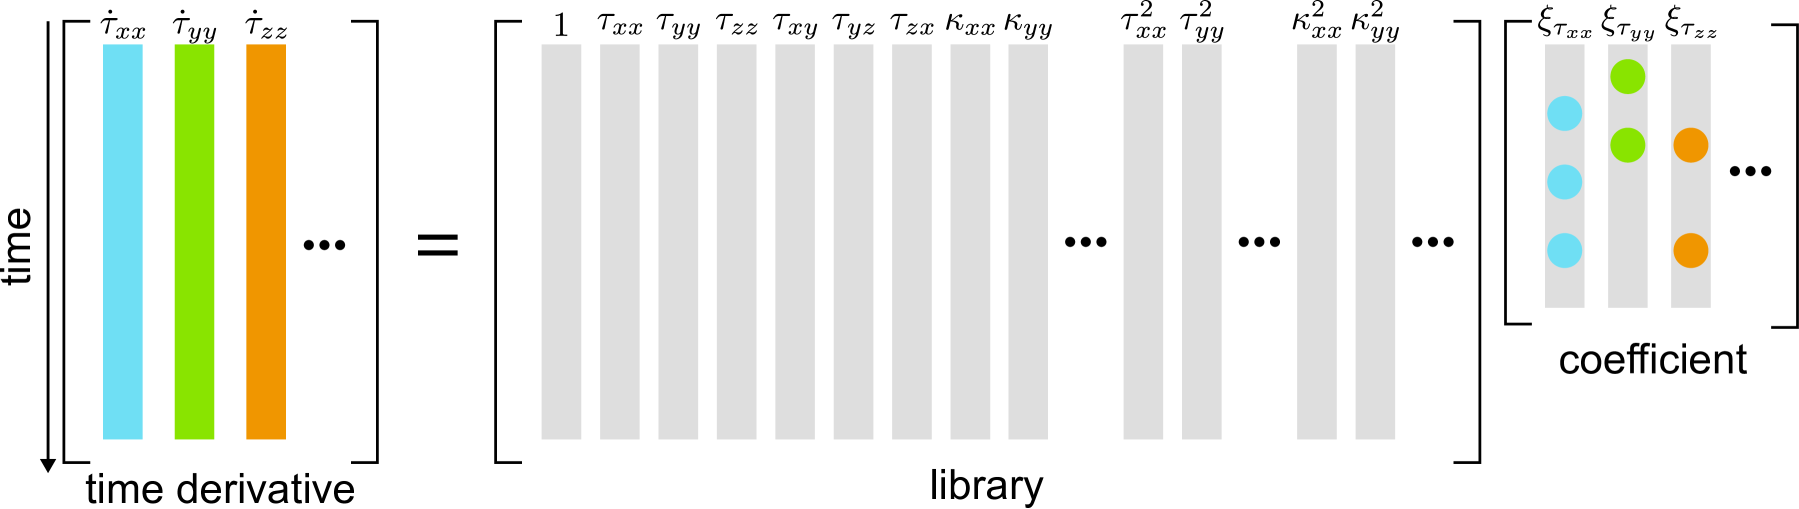
\includegraphics[width=0.8\textwidth]{Fig/xianxingxishu.png}
	\FigureBicaption{\label{xianxingxishu} Rheo-SINDy的示意图}{Schematic illustration of Rheo-SINDy}
\end{figure}
\begin{figure}[htbp]
	\centering
	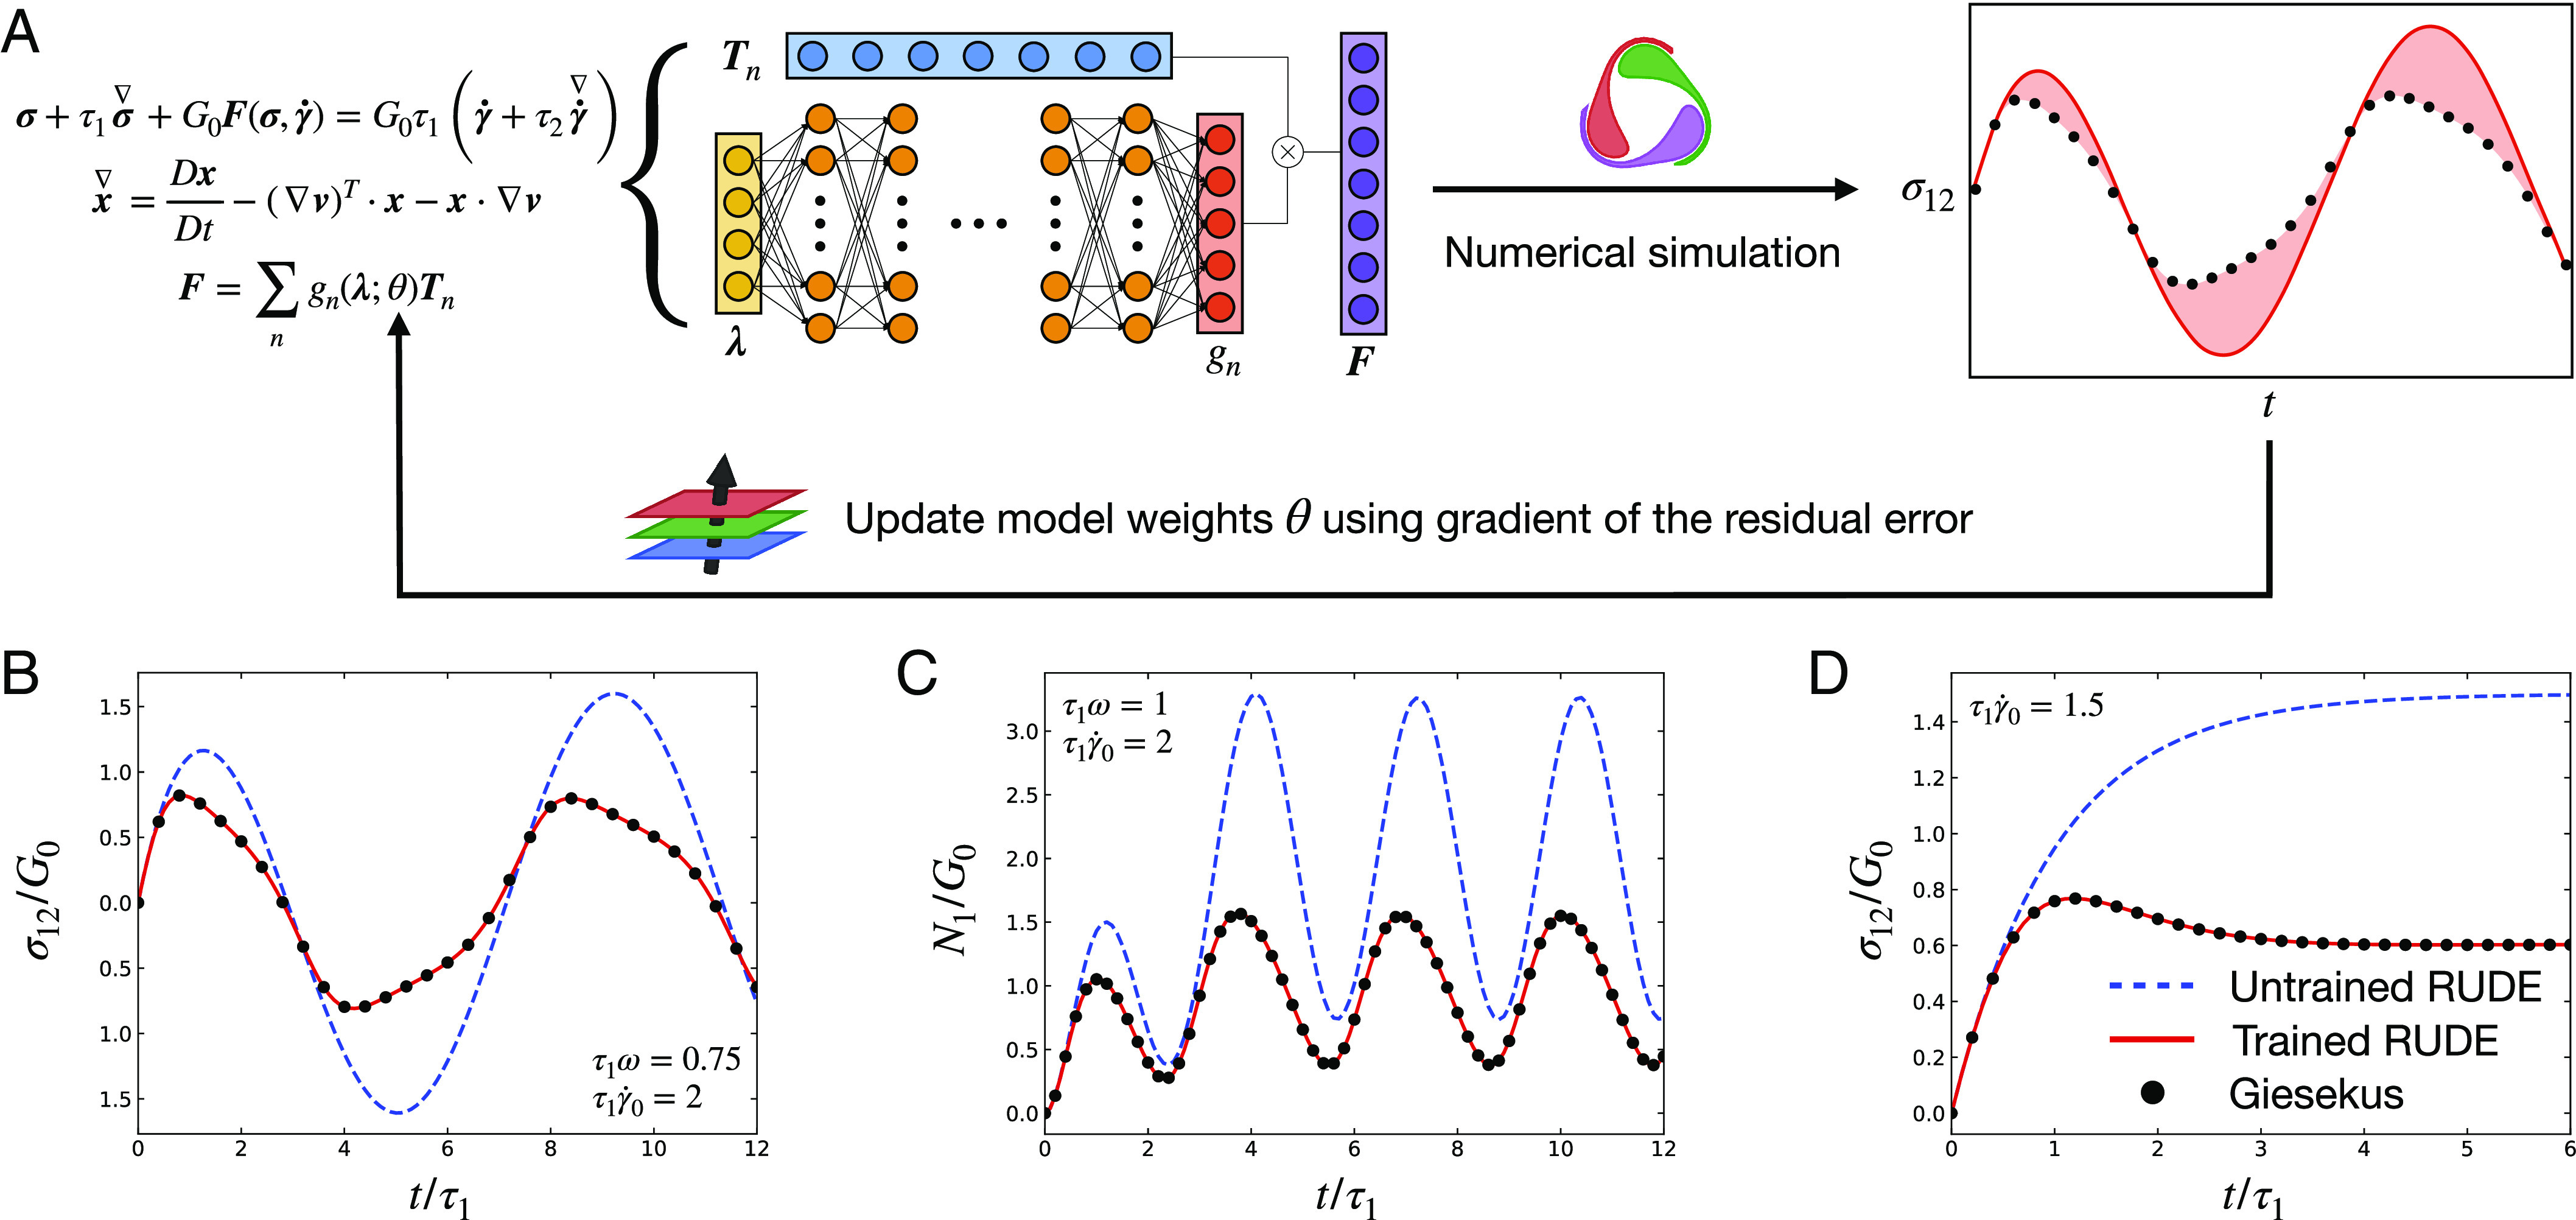
\includegraphics[width=0.8\textwidth]{Fig/pnas.2304669120fig01.jpg}
	\FigureBicaption{\label{lennon} (A) RUDE 训练循环示意图(B–D)基于Giesekus模型合成LAOS数据训练的RUDE评估结果,黑色圆圈:测试数据;红色线条:训练后的RUDE;蓝色线条:未训练的 RUDE(B) 中间频率下的剪切应力响应(C) 训练频率下的法向应力(D) 稳态剪切流启动时的剪切应力响应}{(A) Schematic depiction of a RUDE within the training loop (B–D) Evaluation of a RUDE trained on synthetic LAOS data for the Giesekus model,Black circles: test data; red lines: trained RUDE; blue lines: untrained RUDE (B) Shear stress response at an intermediate frequency (C) Normal stress at a training frequency (D) Shear stress during startup of steady shear flow}
\end{figure}
机器学习技术的另一个重要应用在于发现闭式本构关系,这些关系从数学上描述了应力和变形之间的关联。这一过程通常通过分析实验数据并结合非线性动力学稀疏识别(SINDy)和符号回归等技术来实现。在这些方法中,通常采用多步骤流程:首先从广泛的潜在函数列表中筛选出最重要的候选函数,然后精确恢复这些函数的参数,以最简洁的形式描述动力学系统。例如,SINDy方法被直接扩展到流变学应用中,开发了一种称为Rheo-SINDy的稀疏识别方法,用于从已知方程库生成的流变学数据中恢复本构方程。然而,现有方法在处理不完整、稀缺或噪声数据时面临挑战,特别是需要数值微分来计算导数以构建控制方程。这一问题可以通过结合自动微分功能的物理信息神经网络(PINN)来解决,从而避免数值微分的需求。这种组合方法被称为PINN-SR(具有稀疏回归的PINN),已成功应用于从模型弹性粘塑性流体的实验数据中提取精确的本构关系。

尽管目前大多数机器学习技术(无论是数据驱动还是物理信息)都集中在单个标量分量(如剪切应力、微观结构参数或粘度)作为流变学特征,并与粘度流动和体材料函数预测相关,但真正可推广的流变学机器学习技术必须具备张量性质,并避免客观性问题。Lennon等人提出的RUDE框架优雅地解决了这些基本约束,构建了包含物理信息的可学习模型,同时对特定实验协议或流动运动学的细节保持不可知。在该框架中,广义粘弹性模型中的未知非线性项被表示为张量基函数的线性组合,这些函数强制执行对称性和框架不变性等物理约束,而张量基函数的系数则通过神经网络输出建模。RUDE框架的一个显著优势在于,其预测不仅能够推广到观测域之外,还可以扩展到应力张量的其他分量,从而实现完全解析的流动预测。这种能力使得RUDE在流变学应用中展现出强大的泛化能力和实用性。
\subsubsection{其他物理信息深度学习模型}
近年来,深度神经算子作为一种新的机器学习模型被提出,用于隐式学习物理现象的解算子。与使用有限维向量空间的标准神经网络不同,神经算子学习函数空间之间的映射。典型的架构包括DeepONet和傅里叶神经算子(FNO)及其变体。DeepONet由两个子网络组成:分支网络和中继网络,分别提取输入函数和输入坐标的潜在表示,并通过点积合并输出。FNO通过在傅里叶空间中参数化积分核来实现高效的架构。神经算子可以作为隐藏控制方程的隐式解算子,使其成为理解复杂物理系统的强大工具。它们可以与物理场和其他域约束结合,以获得高保真解和良好的泛化能力。

神经算子在简洁且准确地学习复杂动力学方面表现出色,已在流体力学应用中得到验证,如天气预报和碳捕获的储层工程。然而,在复杂流体领域的应用仍有限。例如,Jin等人使用DeepONet框架从稀疏但高质量的实验数据中学习了建筑超材料的微观结构与机械响应之间的关系,Rashid等人采用FNO架构预测了数字复合材料中的应力和应变场。FNO的扩展,如隐式傅里叶神经算子(IFNO),已被证明可以预测不可见载荷条件下的材料响应,并且同样适用于流变学应用。在IFNO中,层之间的增量由积分算子建模,因此所得架构可以解释为未知控制定律的定点方法。与传统的本构模型相比,这种方法将预测误差减少了十倍。Howard等人还应用了模型算子回归(MOR-physics)框架,从单分散和双分散悬浮液中的体积分数和速度测量中学习粒子应力。

\section{本课题研究介绍}
\subsection{研究内容}
本文旨在通过多方法融合的系统性研究,探索深度学习在模拟数据和实验数据下本构方程的建模与评估,文章主要结构如下,研究路线如图\ref{HolisticResearchFramework}所示。

第一章首先综述了流变学研究的基本问题和应用方向。其次讨论了本构方程理论的发展,经典本构方程的发展历史,数学形式,适用范围等。然后综述了本构方程的研究方法,包括传统的数值方法和近年来被广泛研究的数据驱动机器学习方法。最后综述了将物理约束引入机器学习方法的研究现状,并简述了本文后续的课题设计方案。

第二章主要介绍了本文课题中主要使用的各类算法,从算法理论到选型依据做了综述讨论。
\begin{figure}[htbp]
	\centering
	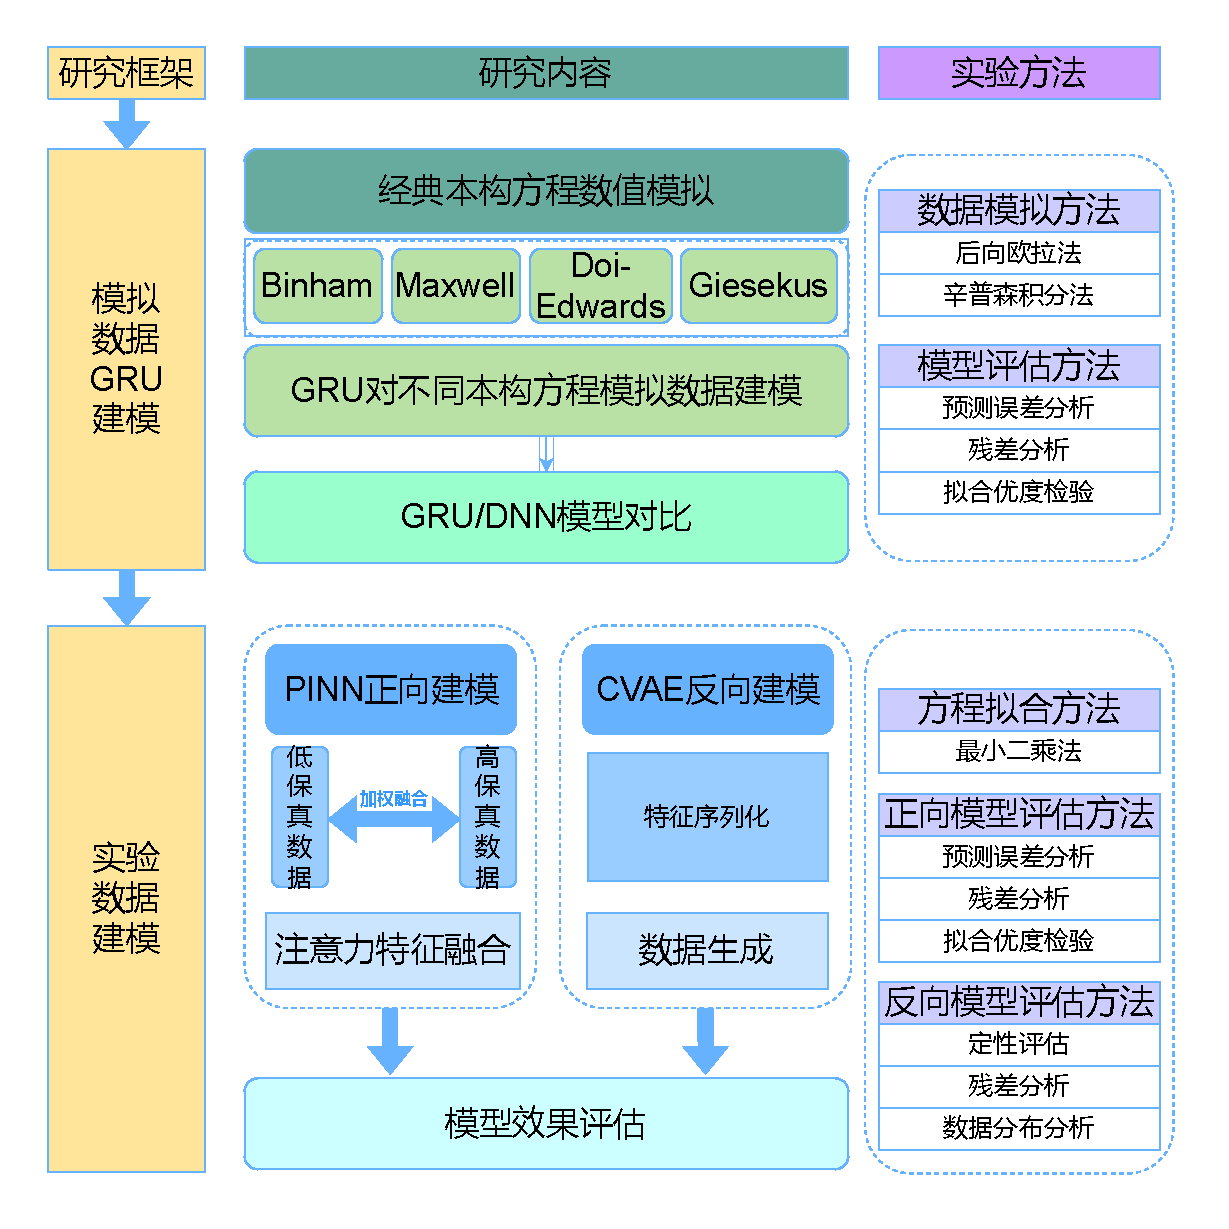
\includegraphics[width=0.8\textwidth]{Fig/HolisticResearchFramework.drawio.pdf}
	\FigureBicaption{\label{HolisticResearchFramework} 研究路线图}{Research roadmap}
\end{figure}
第三章介绍了本文的第一部分工作,使用门控循环单元(GRU)对经典本构方程的模拟数据进行深度学习建模,并使用各种指标对模型性能进行评估。具体来说,首先基于经典本构方程(Binham模型、Maxwell模型、Doi-Edwards模型、Giesekus模型),采用后向欧拉法和辛普森积分法等数值模拟方法生成模拟数据,并划分训练集、验证集、测试集。随后使用GRU分别对不同的模型模拟数据进行建模,训练后使用测试集进行模型的评估,采用决定系数(R$^2$)、平均绝对误差(MAE)、平均绝对百分比误差(MAPE)
等指标,对模型性能进行定量评估。同时在相同的数据集上使用普通深度神经网络(DNN)进行训练,将两套模型进行比较,以验证GRU模型在处理复杂非线性时间依赖性流变学本构方程时的优势。

第四章介绍了本文的第二部分工作,针对黏弹性凝胶材料的真实实验流变数据进行物理信息神经网络(PINN)的建模,在Mahmoudabadbozchelou等人的模型基础之上,进一步优化PINN的模型,采用可学习的损失权重进行损失函数的优化,探究PINN对特定参数下凝胶材料模量及损耗因子的预测能力。随后,采用条件变分自编码器(CVAE)反向建立生成式模型,通过这个模型生成特定流变学数据下的制备参数,并进行生成效果评估。

\subsection{研究创新点}
\begin{enumerate}[topsep = 0 pt, itemsep= 0 pt, parsep=0pt, partopsep=0pt, leftmargin=44pt, itemindent=0pt, labelsep=6pt, label=(\arabic*)]
	\item 本文采用门控循环单元(GRU),通过其门控机制捕捉时间序列数据中的时间依赖性,使模型更贴近复杂流体的物理特性。
	\item 优化Mahmoudabadbozchelou提出的物理信息神经网络(PINN),引入可学习的权重损失以缓解多损失函数的梯度消失问题,并结合注意力特征融合解决实验数据稀疏问题。
	\item 使用CVAE反向建模,以流变学特性反预测制备参数,辅助实验设计。
\end{enumerate}
\subsection{研究意义}
传统机器学习方法在流变学建模中往往局限于单点预测,难以捕捉复杂流体的时间依赖性,而本文采用门控循环单元(GRU)进行建模,充分利用其时间序列处理能力,使模型更贴近黏弹性材料的流变学特性。这一研究不仅拓展了深度学习在流变学领域的应用范围,还为复杂流体建模提供了新的理论支持。随着计算机科学的发展,自注意力机制(如Transformer)在自然语言处理等领域展现了强大的长程依赖捕捉能力。尽管受限于流变学数据的稀缺性,本文未直接采用Transformer架构,但通过探索能够解决长期序列依赖的模型,为未来本构方程建模的研究指明了方向。这一思路有望进一步推动流变学本构建模的发展,为解决复杂流体建模问题提供更强大的工具。

本文通过优化物理信息神经网络(PINN),引入可学习权重和注意力特征融合,为小样本学习提供了新的解决方案,提升了模型在数据稀缺情况下的性能。同时,利用条件变分自编码器(CVAE)进行反向建模,以流变学特性反推制备参数,为实验设计提供了理论支持。这些研究不仅推动了流变学建模方法的进步,还为材料科学和工程领域的实验优化提供了新的思路,具有一定的理论意义和实践价值。%第一章
\chapter{算法介绍}
\section{引言}
本文基本的研究思路是使用数值模拟算法和深度学习算法来研究流变学本构方程建模的问题。本文的实验研究第一部分基于动态时序建模理论和PINN的物理约束理论,构建物理信息-门控循环单元网络(PI-GRU)的预测模型,通过深度学习算法处理数值模拟生成的时变本构关系数据,重点解析循环神经网络在时间序列建模中的特征提取机制,主要涉及的算法模型有GRU算法模型,本章同时综述了时间序列数据的其他深度学习算法。第二部分引入物理约束的智能建模策略,针对实际流变实验数据构建融合物理信息的混合神经网络模型,重点整合了物理信息神经网络(PINN)的微分方程嵌入技术、基于注意力机制驱动的多源特征融合方法,以及结合条件变分自编码框架(CVAE)的生成式建模策略,实现物理规律约束下的数据-模型双驱动建模。

本章将在此基础上,对研究中所涉及的关键算法进行理论概述,并阐述实验中算法选型的依据,以系统性地综述相关领域的研究进展,为后续研究奠定理论基础。
\section{算法介绍}
\subsection{时间序列数据介绍}
时间序列数据是指在一系列时间点上按时间顺序排列的数据点集合。这些数据点通常是连续或定期记录的,反映了某个变量随时间的变化情况。在流变学研究中,时间域的应力应变数据在小应变时满足玻尔兹曼叠加原理,即当前应力状态为之前所有应变历史的线性和\cite{boltzmannZurTheorieElastischen1878}。大应变时应力应变数据虽然不满足玻尔兹曼的线性叠加,但是依旧可以表示为过去应变历史的非线性关系叠加。

\subsection{循环神经网络}
\subsubsection{简单RNN}
循环神经网络(RNN)是一种专门处理序列数据的神经网络结构,其核心在于利用循环结构捕捉时间或顺序上的依赖关系\cite{elmanFindingStructureTime1990}。RNN的基本结构由输入层、隐藏层和输出层组成(图\ref{rnn_gru illustration}(a))。隐藏层中的神经元不仅接收来自输入层的信号,还接收来自前一时刻隐藏层的信号。这种循环连接使得RNN能够捕获序列中的时间依赖关系。
RNN的数学模型可以通过公式\eqref{eq:rnnht}描述:
\begin{align}
   & \mathbf{h}_t = \sigma(\mathbf{W}_{xh} \mathbf{x}_t + \mathbf{W}_{hh} \mathbf{h}_{t-1} + \mathbf{b}_h) \label{eq:rnnht} \\
   & {\mathbf{o}_t = \mathbf{W}_{ho} \mathbf{h}_t + \mathbf{b}_o} \label{eq:rnnot}
\end{align}
其中$\mathbf{h}_t$ 是时刻 $t$ 的隐藏状态,$\mathbf{x}_t$ 是时刻 $t$ 的输入,$\mathbf{o}_t$ 是时刻 $t$ 的输出,$\mathbf{W}_{xh}$ 是输入到隐藏层的权重矩阵,$\mathbf{W}_{hh}$ 是隐藏层到隐藏层的权重矩阵,$\mathbf{W}_{ho}$ 是隐藏层到输出层的权重矩阵,$\mathbf{b}_h$ 和 $\mathbf{b}_o$ 是偏置。$\sigma$是激活函数,通常使用 $\tanh$ 或 $\text{ReLU}$。RNN 的训练过程通常使用反向传播算法。通过计算梯度来更新权重矩阵,从而最小化损失函数。

在简单的RNN中,存在梯度消失问题,这主要源于反向传播过程中梯度的连乘效应\cite{schmidhuber1997long}。损失函数 $L$ 对 $\mathbf{W}_{hh}$ 的梯度可以表示为公式\eqref{eq:rnngradient}:
\begin{align}
  \frac{\partial L}{\partial \mathbf{W}_{hh}} = \sum_{t=1}^{T} \frac{\partial L}{\partial \mathbf{h}_t} \cdot \frac{\partial \mathbf{h}_t}{\partial \mathbf{W}_{hh}} \label{eq:rnngradient}
\end{align}
展开后,隐藏状态关于$\mathbf{W}_{hh}$ 的导数为公式\eqref{eq:rnngradient2}:
\begin{align}
  \frac{\partial \mathbf{h}_t}{\partial \mathbf{W}_{hh}} = \sigma'(\mathbf{W}_{hh} \mathbf{h}_{t-1} + \mathbf{W}_{xh} \mathbf{x}_t + \mathbf{b}_h) \cdot \mathbf{h}_{t-1}^T \label{eq:rnngradient2}
\end{align}
注意到,$\frac{\partial L}{\partial \mathbf{h}_t}$依赖于前一个时间步的梯度,如公式\eqref{eq:rnngradient3}:
\begin{align}
  \frac{\partial L}{\partial \mathbf{h}_t} = \frac{\partial L}{\partial \mathbf{h}_{t+1}} \cdot \frac{\partial \mathbf{h}_{t+1}}{\partial \mathbf{h}_t} = \frac{\partial L}{\partial \mathbf{h}_{t+1}} \cdot \mathbf{W}_{hh} \cdot \sigma'(\mathbf{h}_t) \label{eq:rnngradient3}
\end{align}
这表明梯度在通过时间反向传播时会乘以$\mathbf{W}_{hh}$。
从时间$t$到时间$T$的梯度可以表示为公式\eqref{eq:rnngradient4}:
\begin{align}
  \frac{\partial L}{\partial \mathbf{h}_t} = \left( \prod_{k=t+1}^{T} \mathbf{W}_{hh} \cdot \sigma'(\mathbf{h}_{k-1}) \right) \cdot \frac{\partial L}{\partial \mathbf{h}_T} \label{eq:rnngradient4}
\end{align}
其中乘积 $\prod_{k=t+1}^{T} \mathbf{W}_{hh} \cdot \sigma'(\mathbf{h}_{k-1})$在某些情况下可能会非常小,例如如果 $\mathbf{W}_{hh}$的特征值小于1,那么随着$(T - t)$的增加,$\mathbf{W}_{hh}^{T-t}$将呈指数级减小并趋近于零。
如果反向传播过程中每一项都小于1,那么整个乘积将随着 $(T - t)$的增加呈指数级减小。
这意味着对于远离输出端的时间步$t$,梯度$\frac{\partial L}{\partial \mathbf{h}_t}$将非常小,导致权重更新几乎停止,这就是RNN的梯度消失问题。由于RNN为了捕捉时间依赖性,我们不可避免地设置长时间步,这导致RNN梯度消失问题几乎难以避免。

\subsubsection{GRU}
为了解决简单RNN的梯度消失问题,Schmidhuber等提出了长短期记忆网络(Long Short-Term Memory,LSTM)\cite{schmidhuber1997long}。LSTM通过引入门控机制来控制信息的流动,从而有效地缓解梯度消失问题。LSTM的核心结构包括输入门、遗忘门和输出门,这些门控机制能够有效地控制信息的流动,从而捕获长期依赖关系。

LSTM虽然通过引入门控机制有效地解决了简单RNN中的梯度消失问题,但在实际应用中仍然存在一些问题。LSTM包含三个门(输入门、遗忘门、输出门),导致其参数数量较多,增加了模型的复杂度和计算成本。由于LSTM的复杂结构,其训练和推理速度相对较慢,尤其是在处理大规模数据时。为了解决LSTM的上述问题,Cho等提出了GRU作为LSTM的简化版本\cite{choLearningPhraseRepresentations2014}(图\ref{rnn_gru illustration}(b))。GRU的设计初衷是为了简化LSTM的结构,同时保持其捕获长期依赖关系的能力。GRU只有重置门(Reset Gate)和更新门(Update Gate)两种门控单元,与LSTM相比,GRU的参数数量较少,训练和推理速度更快。重置门的计算公式为公式\eqref{eq:grureset}。
\begin{align}
  \mathbf{r}_t = \sigma(\mathbf{W}_r \mathbf{x}_t + \mathbf{U}_r \mathbf{h}_{t-1} + \mathbf{b}_r) \label{eq:grureset}
\end{align}
更新门的计算公式为公式\eqref{eq:gruupdate},重置门决定了前一时间步的隐藏状态在多大程度上被忽略。当重置门的输出接近0时,网络倾向于"忘记"前一时间步的信息,仅依赖于当前输入;而当输出接近1时,前一时间步的信息将被更多地保留。
更新门决定了多少过去的信息将被保留,而新信息将占据多少比例。当更新门的输出接近1时,新的隐藏状态几乎等同于旧的隐藏状态,从而实现了长期依赖的捕捉;当更新门的输出接近0时,新的隐藏状态将主要由当前输入决定。
\begin{figure}[htbp]
  \centering
  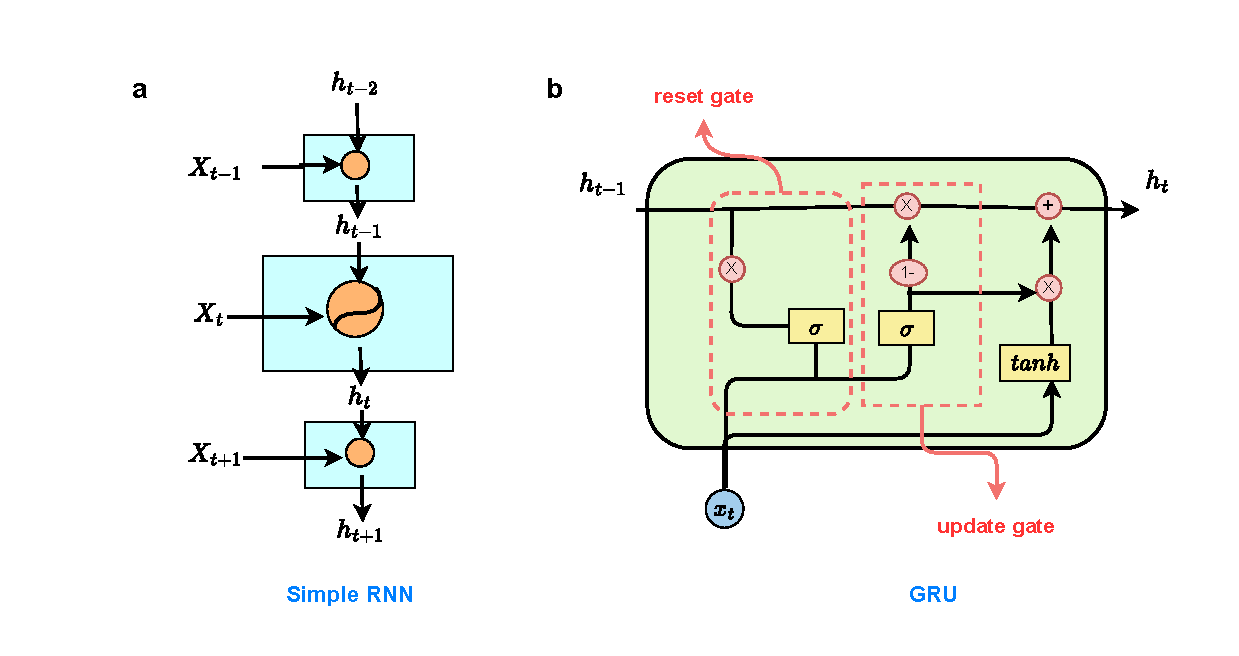
\includegraphics[width=0.9\textwidth]{Fig/rnn-gru.pdf}
  \FigureBicaption{\label{rnn_gru illustration}(a)RNN 示意图 ;(b)GRU 示意图}{Schematic illustration of (a) RNN and (b) GRU}
\end{figure}
\begin{align}
  \mathbf{z}_t = \sigma(\mathbf{W}_z \mathbf{x}_t + \mathbf{U}_z \mathbf{h}_{t-1} + \mathbf{b}_z) \label{eq:gruupdate}
\end{align}
候选隐藏状态决定了当前时间步的新信息,如公式\eqref{eq:gruhih}所示。
\begin{align}
  \tilde{\mathbf{h}}_t = \tanh(\mathbf{W}_h \mathbf{x}_t + \mathbf{U}_h (\mathbf{r}_t \odot \mathbf{h}_{t-1}) + \mathbf{b}_h) \label{eq:gruhih}
\end{align}
当前隐藏状态如公式\eqref{eq:gruhi}所示,这里的当前隐藏状态与上文LSTM的隐藏状态含义是一样的。
\begin{align}
  \mathbf{h}_t = (1 - \mathbf{z}_t) \odot \mathbf{h}_{t-1} + \mathbf{z}_t \odot \tilde{\mathbf{h}}_t \label{eq:gruhi}
\end{align}

GRU移除了单元状态的概念,直接从门控单元来计算隐藏状态,GRU 通过重置门和更新门的协同工作,实现了对信息流动的有效控制,使得网络能够在需要时记住长期依赖关系,同时减少梯度消失/爆炸的问题。GRU的结构比LSTM更简单,计算效率更高,因此在实践应用中广受欢迎。本章使用GRU模型进行流变学本构方程的预测建模。

GRU能够有效缓解梯度消失问题的关键在于其更新门机制。我们可以从梯度传播的角度进行分析。对于时间步$t$的隐藏状态$\mathbf{h}_t$,其关于时间步$t-1$的隐藏状态$\mathbf{h}_{t-1}$的梯度可以表示为:
\begin{align}
  \frac{\partial \mathbf{h}_t}{\partial \mathbf{h}_{t-1}} = \frac{\partial[(1 - \mathbf{z}_t) \odot \mathbf{h}_{t-1} + \mathbf{z}_t \odot \tilde{\mathbf{h}}_t]}{\partial \mathbf{h}_{t-1}} \label{eq:grugrad1}
\end{align}

展开上式,可得:
\begin{align}
  \frac{\partial \mathbf{h}_t}{\partial \mathbf{h}_{t-1}} & = (1 - \mathbf{z}_t) + \frac{\partial \mathbf{z}_t}{\partial \mathbf{h}_{t-1}} \odot (\tilde{\mathbf{h}}_t - \mathbf{h}_{t-1}) + \mathbf{z}_t \odot \frac{\partial \tilde{\mathbf{h}}_t}{\partial \mathbf{h}_{t-1}} \label{eq:grugrad2}
\end{align}

注意到第一项$(1 - \mathbf{z}_t)$是一个直接传递梯度的路径,这意味着当$\mathbf{z}_t$接近0时,前一时间步的隐藏状态几乎可以不经修改地直接传递到当前时间步。这种线性路径允许梯度在长时间步之间直接流动,有效避免了梯度消失问题。

与简单RNN相比,在RNN中,隐藏状态的梯度如公式\eqref{eq:rnngrad}所示:
\begin{align}
  \frac{\partial \mathbf{h}_t}{\partial \mathbf{h}_{t-1}} = \mathbf{W}_{hh} \cdot \sigma'(\mathbf{W}_{hh} \mathbf{h}_{t-1} + \mathbf{W}_{xh} \mathbf{x}_t + \mathbf{b}_h) \label{eq:rnngrad}
\end{align}

在RNN中,梯度必须经过非线性激活函数的导数$\sigma'$和权重矩阵$\mathbf{W}_{hh}$,这些连续的乘积会导致梯度消失。而在GRU中,由于更新门的存在,梯度可以通过$(1 - \mathbf{z}_t)$这一线性路径直接传递,从而在很大程度上缓解了梯度消失问题。

更新门$\mathbf{z}_t$实际上充当了一个自适应的开关,当需要保留长期记忆时,$\mathbf{z}_t$接近0,梯度可以几乎无损地传递;当需要关注当前输入时,$\mathbf{z}_t$接近1,网络会更多地考虑新信息。这种自适应的门控机制是GRU能够有效处理长期依赖关系的关键所在。

此外,重置门$\mathbf{r}_t$通过控制前一隐藏状态对候选隐藏状态的影响程度,使网络能够在需要时"重置"先前的记忆,这进一步增强了GRU捕获复杂时序模式的能力。综合来看,GRU通过其简化但高效的门控机制,在保持捕获长期依赖能力的同时,显著缓解了传统RNN中的梯度消失问题,使其成为时序建模的强大工具。
\subsection{其他时间序列算法}
在深度学习领域,针对时间序列数据的处理方法已呈现出多样化的趋势。除了传统的循环神经网络(RNN)及其变体,近年来研究人员提出多种新型网络架构,包括卷积神经网络(CNN)、Transformer以及Mamba网络等,这些方法在时间序列分析中展现出显著的优势。

卷积神经网络(CNN)最初是为图像处理任务设计的,但其在时间序列分析中的应用也取得了显著成效\cite{lecun1998gradient}。通过引入一维卷积操作,CNN能够有效地从时间序列数据中提取局部特征。由于卷积操作具有权值共享的特性,CNN在处理长序列数据时表现出较高的计算效率,并且能够有效规避传统RNN中常见的梯度消失或梯度爆炸问题。通过多层卷积结构的堆叠,CNN能够捕获更为复杂的时间依赖性,进而在语音识别、金融预测等实际应用中表现出优异的性能\cite{li2021survey}。

Transformer模型是近年来在自然语言处理(NLP)领域取得突破性进展的架构,其核心在于自注意力机制(Self-Attention)\cite{Vaswanietal2017Attention}。与传统的RNN类模型不同,Transformer摒弃了序列顺序处理的限制,转而通过全局上下文信息建模序列中各元素之间的依赖关系。这种机制使得Transformer能够并行处理长序列数据,并捕获全局时序特征。在时间序列分析任务中,Transformer通过自注意力机制能够聚焦于序列中的关键时间点,从而有效建模时序依赖性和非线性关系。这一特性使其在机器翻译、语音识别等任务中超越了传统模型的表现。

Mamba网络是近年来提出的一种新型时间序列处理架构,专门针对复杂时间序列数据的高效建模而设计\cite{gu2024mamba}。与传统的RNN或CNN模型相比,Mamba网络通过引入多尺度时序建模策略,能够同时捕获时间序列中不同时间尺度的特征。这种多尺度建模方法不仅增强了模型的表达能力,还提升了其在处理多变且复杂时序数据时的鲁棒性。这一特性使其在金融市场分析、气象预测等领域展现出广阔的应用前景。

这些方法不仅拓展了时间序列建模的理论边界,也为实际应用提供了更为强大的工具。本文的研究工作是选择一种可以处理时间序列的算法来对数值模拟的流变学数据进行建模预测,样本量在万级,属于中小规模数据集,综合考虑算法时空间复杂度和训练成本,选择RNN中的GRU作为基础算法模型。未来针对更多流变学数据和复杂场景,可以进一步研究其他前沿模型的应用。
\section{物理信息神经网络}
\subsection{理论基础}
物理信息神经网络(Physics-Informed Neural Networks, PINN)是一种融合深度学习与物理原理的混合建模范式,专门用于解决偏微分方程(PDE)\cite{raissiPhysicsinformedNeuralNetworks2019a}。与传统的纯数据驱动神经网络不同,PINN通过在训练过程中引入物理约束条件,使模型不仅能从数据中学习统计规律,还能满足底层物理定律,从而显著提高模型的泛化能力和预测精度。PINN的核心思想在于将物理定律(通常表现为偏微分方程)作为先验知识嵌入神经网络的损失函数中,通过同时最小化数据拟合误差和物理方程残差来训练模型。这种方法使得PINN在保持神经网络高度非线性表达能力的同时,确保模型预测结果符合物理定律,增强了模型的物理一致性和可解释性。
\begin{figure}[htbp]
  \centering
  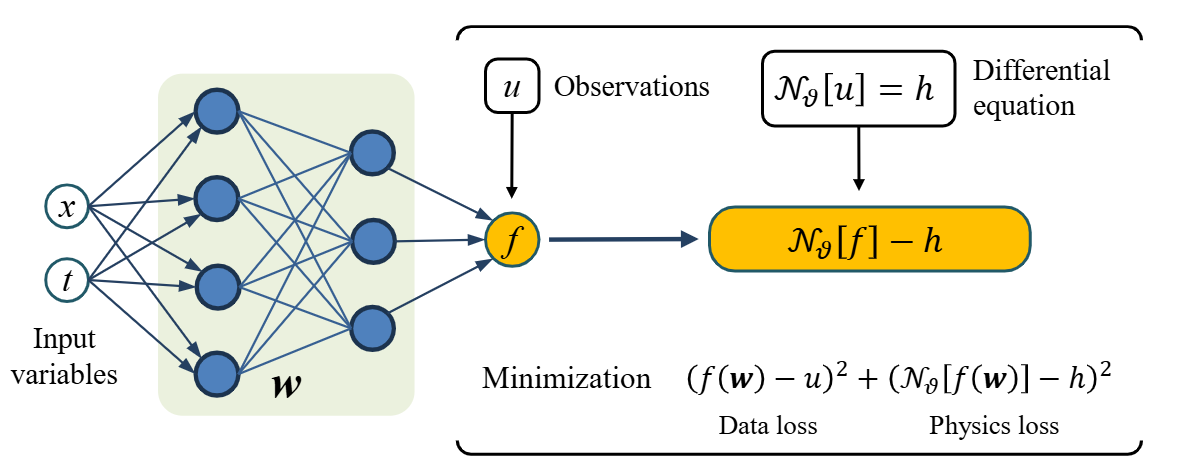
\includegraphics[width=0.8\textwidth]{Fig/pinn_logo.png}
  \FigureBicaption{\label{pinn illustration}PINN 示意图\cite{cuomoScientificMachineLearning2022}}{Schematic illustration of PINN\cite{cuomoScientificMachineLearning2022}}
\end{figure}
PINN的显著优势在于其能通过物理方程进行半监督或无监督训练,大幅降低对大规模标注数据的依赖。此外,PINN能确保模型预测符合物理定律,有效避免了纯数据驱动模型可能产生的物理不合理解。然而,PINN在处理高维复杂问题时仍面临训练收敛性和求解精度等挑战。
\subsection{损失函数构建}
PINN的核心在于其损失函数的精确构建。与传统深度神经网络(DNN)仅依赖数据损失$\mathcal{L}_{data}$不同,PINN的损失函数如公式\eqref{eq:pinnloss}所示,由数据损失和物理损失两部分组成,其中$\lambda$为平衡两种损失的权重系数。
\begin{align}
  \mathcal{L} = \mathcal{L}_{data} + \lambda\mathcal{L}_{physics} \label{eq:pinnloss}
\end{align}
数据损失用于量化神经网络预测值与实际观测数据之间的偏差,通常采用均方误差(MSE)作为度量标准,如公式\eqref{eq:mse}所示。其中,$N_d$表示观测数据点的数量,$u(x_i, t_i)$表示神经网络在点$(x_i, t_i)$处的预测值,$u_i$为对应位置的真实观测值。
\begin{align}
  \mathcal{L}_{data} = \frac{1}{N_d} \sum_{i=1}^{N_d} \left( u(x_i, t_i) - u_i \right)^2 \label{eq:mse}
\end{align}
物理损失则确保神经网络的预测结果满足基本物理定律,通常通过计算物理方程的残差实现。以纳维-斯托克斯方程为例,其物理损失可表示为公式\eqref{eq:physicsloss}。本质上,物理损失反映了神经网络预测值在满足物理方程时的残差大小,残差越小,表明预测结果越符合物理规律。
\begin{align}
  \mathcal{L}_{physics} = \frac{1}{N_p} \sum_{j=1}^{N_p} \left( \frac{\partial u}{\partial t} + (\mathbf{u} \cdot \nabla) \mathbf{u} - \nu \nabla^2 \mathbf{u} - \nabla p + \mathbf{f} \right)^2 \bigg|_{(x_j, t_j)} \label{eq:physicsloss}
\end{align}
\subsection{前沿发展与优化方向}
公式\eqref{eq:pinnloss}中的权重参数$\lambda$控制物理损失与数据损失之间的相对重要性。当$\lambda$较大时,模型更倾向于满足物理约束;反之则更注重数据拟合。初期PINN研究常忽略此权重调节,使最终损失函数易受数据规模影响。特别是在多保真度建模中,若使用高保真数据计算数据损失,低保真数据计算物理残差,则当低保真数据量远大于高保真数据时,权重参数的精确设定变得尤为关键,以避免梯度消失或主导问题\cite{luDeepXDEDeepLearning2021}。

针对$\lambda$的优化,传统方法依赖经验调参,不仅缺乏理论依据,且耗时费力。近年来,自动化权重确定方法已成为研究热点。Farmer等人提出了一种经验性损失权重优化方法,用于PINN求解激光生物效应的1D热方程\cite{farmerEmpiricalLossWeight2024},通过自动归一化各损失项以保证平衡。Xiang等人开发了自适应损失平衡方法(lbPINN),基于高斯概率模型定义自适应损失函数\cite{xiangSelfadaptiveLossBalanced2022},该方法在每个训练周期中基于最大似然估计更新损失项权重,实验证明其在多种方程求解中优于传统PINN。Song等人提出基于损失注意力的PINN架构(LA-PINN),为每个损失项配备独立的损失注意力网络\cite{songLossattentionalPhysicsinformedNeural2024},通过将训练点的平方误差动态加权,显著提高了预测精度和收敛速度。本研究借鉴并简化了Song的方案,实现了具有可学习权重的PINN框架。

在处理高维复杂偏微分方程时,PINN的计算效率仍是一项亟待解决的挑战。未来研究需重点提升计算性能以应对大规模问题\cite{Shah2024BenchmarkingQA-PINN}。此外,PINN在小样本学习方面的表现有待提高,需研发先进的自适应采样和数据增强技术,降低对大量训练数据的依赖。复杂物理约束的有效整合也是当前面临的难题,需开发更灵活强大的方法处理复杂方程和边界条件。在多物理场耦合问题中,PINN的应用范围仍较为局限\cite{Hillebrecht2022Certified,Haitsiukevich2023Improved},因此拓展PINN至多物理场耦合问题是解决复杂实际问题的关键研究方向。

\section{特征融合方法}
\subsection{简单特征融合}
特征融合(Feature Fusion)是深度学习中一种重要的技术,旨在将来自不同来源或不同层次的特征进行组合,以创建一个捕获集体信息的统一表示。这种技术通过利用来自不同特征集的互补信息,能够显著增强模型的性能。

简单的特征融合方法包括Concat、Add和Hadamard Product等。其中,Concat是将两个特征向量拼接在一起,如公式\eqref{eq:concat},适用于需要保留两个特征向量的所有信息的场景。例如,在流体力学中,当需要同时考虑不同物理场(如速度场和压力场)或不同尺度的特征时,Concat 是一种合适的方法。Add是将两个特征向量逐元素相加,如公式\eqref{eq:add},适用于两个特征向量维度相同,且需要强调某些共同特征时。例如,需要将速度场的不同分量相加,可以突出重要的流动特征的时候,可以使用Add方法。Hadamard Product是将两个特征向量逐元素相乘,如公式\eqref{eq:hadamard}。当需要突出共同出现的特征并减弱不重要的特征时,Hadamard Product是一种合适的方法。例如,在流体力学中,如果需要将速度场和压力场的特征相乘,希望突出共同的流动特征时,在材料科学中,如果需要将材料编码和组分含量相乘,突出加权的含量特征时,都可以使用Hadamard Product。
\begin{align}
  \mathbf{v} & = [\mathbf{v}_1; \mathbf{v}_2] \label{eq:concat}          \\
  \mathbf{v} & = \mathbf{v}_1 + \mathbf{v}_2    \label{eq:add}           \\
  \mathbf{v} & = \mathbf{v}_1 \odot \mathbf{v}_2     \label{eq:hadamard}
\end{align}
\subsection{注意力特征融合}
深度学习中,注意力特征融合(AFF)是一种重要的技术,它通过引入注意力机制来动态调整特征的权重,从而更好地融合特征\cite{dai2021attentional}。注意力特征融合的核心思想是利用注意力机制来捕获特征之间的关系,从而增强重要特征并减弱不重要的特征。注意力特征融合的数学公式如公式\eqref{eq:attentionsusion}所示,其中$\mathbf{v}_i$为特征向量,$\alpha_i$为注意力权重,$\mathbf{q}$为查询向量,用于计算注意力权重。
\begin{equation}
  \begin{aligned}
     & \mathbf{v} = \sum_{i=1}^{n} \alpha_i \mathbf{v}_i                                                 \\
     & \alpha_i = \frac{\exp(\mathbf{q}^T \mathbf{v}_i)}{\sum_{j=1}^{n} \exp(\mathbf{q}^T \mathbf{v}_j)}
  \end{aligned}   \label{eq:attentionsusion}
\end{equation}

在多尺度特征融合中,注意力机制的应用极大地提升了模型对不同尺度特征的动态权重调整能力,从而更有效地捕获全局和局部信息。这种方法在目标检测和图像分割等任务中表现出色,因为它能够更好地处理不同尺度的目标。例如,CM-UNet模型通过多尺度注意力聚合模块(MSAA),在遥感图像语义分割任务中高效捕捉局部和全局信息,提升了特征表达能力\cite{Cui2023CMUnet}。

在实现注意力特征融合时,通常会使用注意力模块,如自注意力(Self-Attention)或交叉注意力(Cross-Attention)。自注意力机制允许模型在同一个序列内部捕获特征之间的关系,而交叉注意力机制则允许模型在两个不同的序列之间捕获特征之间的关系。例如,交叉注意力可以用于将图像特征与文本特征进行融合,从而实现更准确的图像描述生成。在多模态学习中,交叉注意力机制通过在不同模块之间引入注意力机制,让信息交流更高效,也让模型在处理复杂任务时表现得更出色\cite{rong2023dynstatf}。

此外,注意力特征融合还可以与其他特征融合方法(如Concat和Add)结合使用。例如,在某些模型中,可以先使用Concat将不同来源的特征拼接在一起,然后使用注意力机制对拼接后的特征进行加权,从而进一步增强特征的表示能力。这种方法在多模态学习中特别有用,因为它可以有效地融合来自不同模态的特征。例如,多模态融合网络使用多头自注意力机制来最小化不同模态之间的噪声干扰,并利用局部区域特征表示之间的相关性来提取互补信息\cite{nagrani2021attention}。

总结注意力机制在多尺度特征融合和多模态学习中具有广泛的应用前景,能够显著提升模型的性能和泛化能力。通过合理设计和应用注意力模块,可以更好地捕获和融合不同尺度和模态的特征,从而在各种任务中取得更好的效果。而针对本文流变学的本构建模任务,由于制备参数(分子量、组分比例等)特征存在隐藏联系,但是特征本身非常稀疏,所以采取注意力特征融合的方法,期待显著提高模型的性能和泛化能力。
\section{生成式模型}
\subsection{变分自编码器}
生成式模型是一类能够学习数据生成过程的统计模型。它们通过建模数据的联合概率分布,能够生成与数据相似的新样本。与别判别式模型(关注于建模条件概率分布)不同,生成式模型关注数据的整体结构和分配。

变分自编码器是一种生成模型,结合了自编码器架构和变分推断方法。其核心思想是通过编码器将输入数据映射到潜在变量的分布参数(通常是均值和方差),然后通过解码器从这个分布中采样并重构输入数据变分自编码器(Variational Autoencoder, VAE)的概念最早由Diederik提出。VAE的数学表达式如公式\eqref{eq:vae}所示。其中编码器将输入数据映射到潜在变量空间,解码器将潜在变量映射回原始输入空间。VAE的目标是最小化重构损失和变分下界的差异\cite{kingma2013auto}。
\begin{equation}
  \mathcal{L}(\theta_E, \theta_D) = \mathbb{E}_{q_{\theta_E}(z|x)} \left[ \log p_{\theta_D}(x|z) \right] - D_{KL}(q_{\theta_E}(z|x) \| p(z)) \label{eq:vae}
\end{equation}
重构损失$L_{rec} = \frac{1}{N} \sum_{i=1}^{N} \frac{1}{2} \| x_i - \hat{x}_i \|^2$用于衡量模型输出的重构精度,通常采用均方误差(MSE)或交叉熵等损失函数,变分下界$L_{vae} = \mathbb{E}_{q_{\theta_E}(z|x)} \left[ \log p_{\theta_D}(x|z) \right] - D_{KL}(q_{\theta_E}(z|x) \| p(z))
$用于最大化潜在变量分布的重构似然。为了使 VAE 的训练过程可微分,引入了重参数化技巧。具体来说,假设潜在变量$z$服从均值为$\mu$、方差为$\sigma$的高斯分布,可以通过公式$z = \mu + \sigma \cdot \epsilon$从分布中采样,$\epsilon$是标准正态分布的随机变量。

变分自编码器(VAE)能够生成与训练数据类似的样本,例如人脸、文字等。在标签数据稀缺的情况下,VAE可以利用无标签数据学习数据的潜在结构,从而增强模型的泛化能力。凭借这一特性,VAE在图像生成、数据增强、无监督学习等多个领域展现出广泛的应用潜力,已成为生成模型领域的重要研究方向。
\subsection{条件变分自编码器}
条件变分自编码器(Conditional Variational Autoencoder, CVAE)的概念最早由Sohn等人提出\cite{SohnLee2015ConditionalVAE}。CVAE是VAE的扩展,它在VAE的基础之上引入了条件变量,使得生成的样本可以根据特定条件进行控制。CVAE 的核心思想是将条件变量$y$作为输入的一部分,与输入数据$x$一起编码到潜在变量$z$中,然后通过解码器生成样本。CVAE的目标是最大化条件似然$p(x|y) = \int p(x|z,y) p(z|y) dz$。
\begin{figure}[htbp]
  \centering
  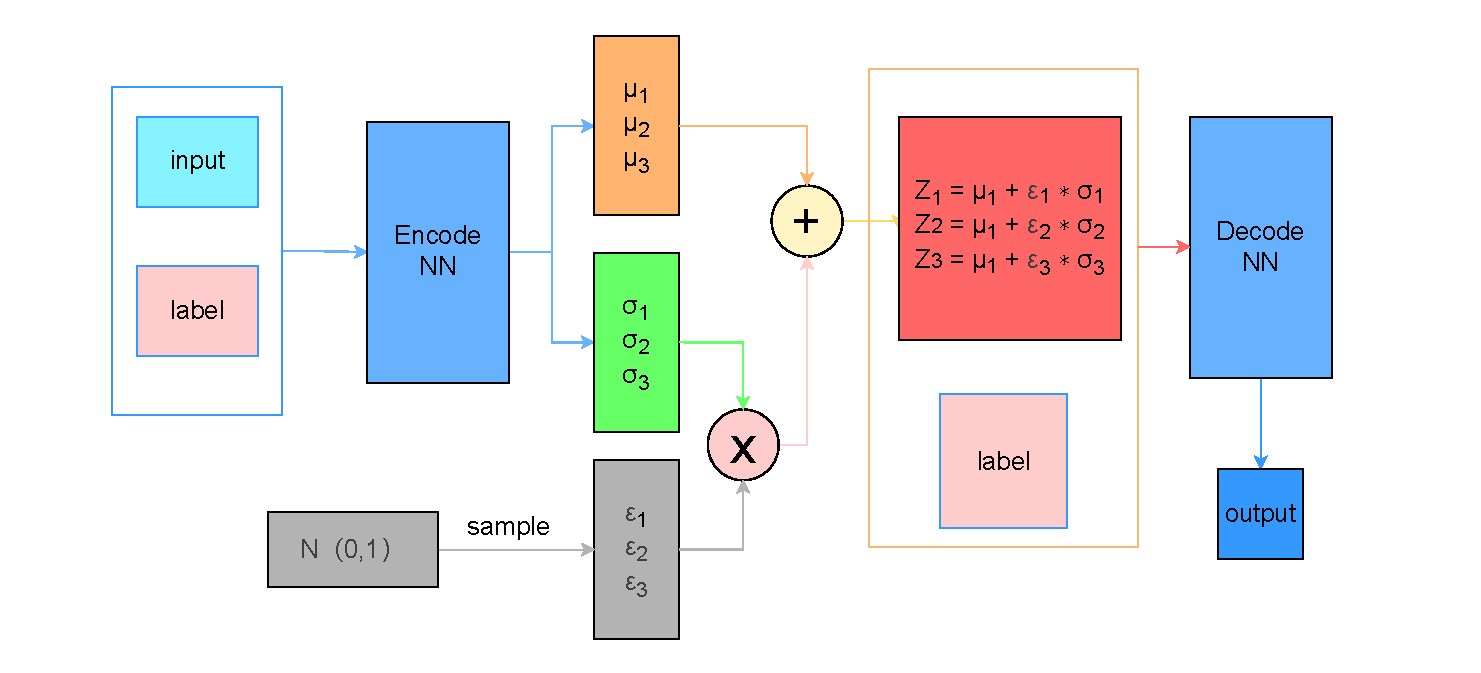
\includegraphics[width=0.8\textwidth]{Fig/CVAE示意图.drawio.pdf}
  \FigureBicaption{\label{cvae illustration}CVAE 示意图}{Schematic illustration of CVAE}
\end{figure}
\begin{equation}
  \mathcal{L}(\theta_E, \theta_D) = \mathbb{E}_{q_{\theta_E}(z|x,y)} \left[ \log p_{\theta_D}(x|z,y) \right] - D_{KL}(q_{\theta_E}(z|x,y) \| p(z|y))
  \label{eq:cvae}
\end{equation}
其中,第一项是重构损失,用于衡量模型输出与真实数据的差异;第二项是 KL散度,用于衡量后验分布与先验分布之间的差异。通过最小化这一损失函数,CVAE能够学习到数据的生成分布,并生成与训练数据类似的样本。
CVAE引入条件变量$y$使得模型能够根据特定条件生成样本,这对于许多实际应用非常重要。例如,在图像生成任务中,条件变量可以控制生成图像的类别或属性。通过指定不同的条件变量,CVAE可以生成不同类别的图像,如不同类型的动物、不同的场景等。这使得CVAE在图像生成领域具有广泛的应用前景。

在自然语言处理任务中,条件变量可以控制生成文本的主题或风格。通过指定不同的条件变量,CVAE可以生成不同主题的文本,如新闻报道、故事、诗歌等。此外,条件变量还可以控制文本的风格,如正式、幽默、悲伤等。这使得 CVAE在自然语言生成领域具有重要的应用价值。

此外,CVAE 还可以在标签数据稀缺的情况下,利用无标签数据学习数据的潜在结构,从而增强模型的泛化能力。在实际应用中,标签数据往往非常稀缺,而无标签数据相对丰富。CVAE可以利用无标签数据学习数据的潜在结构,从而提高模型的性能。这使得CVAE在半监督学习和无监督学习中具有重要的应用价值。

在本文的工作中,我们希望通过已有的流变学性质参数,如特定频率下的储存模量(G')、损耗模量(G")和损耗角正切(tan$\delta$)等,来预测特定的制备参数。CVAE能够将输入数据映射到高维潜在空间,并通过将流变学参数作为条件($y$)输入,生成特定的制备参数。

与传统的深度神经网络(DNN),尤其是回归或分类网络不同,DNN通常直接进行输入到输出的映射,缺乏对潜在空间的建模,因此可能无法捕捉到数据背后复杂的分布。相比之下,CVAE作为生成模型,能够学习输入数据的潜在分布。它不仅依赖于输入数据的特征,还引入了条件信息,使得它能够在潜在空间中生成符合条件的参数,而不仅仅是进行简单的映射。

此外,CVAE通过变分推断捕获数据中的不确定性,能生成多个样本。对于制备参数,可能存在多个合理的组合或生成路径,CVAE通过潜在变量的不同采样来生成这些多样化的样本,从而增强了生成结果的多样性。而传统的DNN模型通常是确定性的,即给定相同的输入总是生成相同的输出,无法有效地表示这种不确定性。

最后,CVAE通过引入变分推断,平衡了重建误差和潜在变量的KL散度,从而在优化过程中不仅考虑了生成结果的质量,还保证了潜在空间的结构化。这使得CVAE能够生成接近原始数据的样本,并通过潜在空间的结构化生成有意义的样本。相比之下,DNN训练时通常只关注误差最小化,缺少对潜在空间结构的显式建模。
\subsection{其他生成式模型}
生成式模型(Generative Models)是机器学习领域的重要研究方向,旨在学习数据的分布特征,从而生成与原始数据相似的新样本。除了变分自编码器(VAE)和条件变分自编码器(CVAE)之外,还有多种生成式模型在不同领域取得了显著成果。

自回归模型基于条件概率链式分解对数据进行建模,通过逐步生成数据单元完成整体构建\cite{bengio2003adaptive}。这类模型在密度估计方面展现出卓越性能,典型代表如PixelCNN和PixelSNAIL已成功应用于图像生成、语音合成等领域。然而其固有特性也带来若干限制:采样过程必须严格遵循序列生成路径,导致高维数据生成效率显著降低;同时模型强制要求将输入数据线性化为固定顺序,这在文本和音频等具有自然时序结构的模态中尚可适用,但对于图像等空间数据而言,最优排列方式的确定缺乏明确依据,且不同的顺序选择可能通过神经网络架构的归纳偏置对最终效果产生潜在影响\cite{bondtaylor2022deep}。

生成对抗网络(Generative Adversarial Networks,GAN)是一种基于博弈论框架的生成模型,其核心由生成器(Generator)与判别器(Discriminator)构成动态博弈系统\cite{NIPS2014_5ca3e9b1}。生成器通过参数化映射函数将潜在空间向量转化为合成数据,旨在捕捉真实数据分布的统计特性;判别器则作为二元分类器,通过迭代优化提升对真实数据与生成数据的鉴别能力。二者在对抗性训练过程中形成"最小-最大"博弈关系:生成器试图生成以假乱真的样本来欺骗判别器,而判别器则持续升级其辨别能力以识别生成样本的统计缺陷,最终推动系统向纳什均衡收敛。相较于传统生成模型,GAN的突出优势在于其能通过对抗机制隐式学习复杂数据分布,生成具有高度视觉保真度的样本(如图像、视频)\cite{Goodfellow2020Generative}。

扩散模型是新一代生成式人工智能的核心范式,其创新性地将数据生成过程建模为物理学启发的渐进式去噪机制\cite{ho2020denoising}。该模型通过构建马尔可夫链,系统性地模拟两个互逆过程:前向扩散阶段将原始数据通过逐步添加高斯噪声退化为随机噪声,反向生成阶段则通过参数化的神经网络学习逆向扩散轨迹,从纯噪声出发通过连续的去噪操作重建出目标数据分布。这种基于随机微分方程(SDE)或概率流常微分方程(ODE)的数学框架,使得模型能够通过变分推断精确优化对数似然下界\cite{song2020score}。相较于GAN,其生成过程具有可解释的物理意义,通过调节去噪步长可实现生成质量与速度的灵活平衡;无需对抗训练避免了模式崩溃风险,确保生成样本的多样性,且理论框架的严密性支持精确的概率密度估计\cite{Cao2024Survey}。
\section{本章小结}
本章系统阐述了深度学习算法在流变学本构建模中的理论基础与应用框架,为后续研究奠定了方法论基础。

首先,针对时序建模技术,本章详细分析了循环神经网络及其变体(尤其是GRU)的核心机制及优势,阐明了其在捕捉流变材料时间依赖性行为方面的适用性,特别是在处理应力松弛等记忆效应现象时的优越性。这些理论为第三章中基于GRU的本构模型识别与预测提供了算法支撑,使我们能够有效处理流变学中的时序依赖性问题。

之后,本章详细介绍了PINN的发展历史、基本数学原理和前沿的优化方向,为物理信息神经网络在流变学中的应用奠定了基础。这一理论框架贯穿第三章与第四章的研究,分别在本构关系预测与材料设计反问题中发挥核心作用,实现了数据与物理规律的有机结合。

在特征融合方法方面,本章介绍了简单特征拼接和多尺度注意力特征融合的方法以及相关的数学原理,并说明了本文后续实验中选取的特征融合方法的依据。这些方法将在第四章中用于整合不同来源和尺度的特征,特别是在处理制备参数与流变性能之间复杂关联时发挥重要作用。

对于生成式模型,本章系统介绍了变分自编码器(VAE)及其条件变体(CVAE)的理论框架,分析了它们在处理流变学参数与制备参数之间映射关系时的优势,尤其是在捕捉多参数组合可能性方面的潜力。这些生成模型理论将在第四章中应用于材料设计的反向问题求解,为从期望性能反推制备参数提供了新途径。

通过构建这一算法体系,本研究为突破传统流变学本构方程的表达限制,发展数据驱动与物理约束相结合的智能建模方法提供了理论支撑和技术路径。本章介绍的各类算法将在后续章节中有机结合,形成完整技术链条。%第二章
\chapter{流变学时间域本构方程的GRU建模研究}
% 3.2表================================================
% % 本节仅展示使用常见的三线表
% \begin{table}
%   \TableBicaption{\label{TDF_para}涵道模型参数}{Parameters of Ducted Fan Model}  % 中英文标题
%   \centering
%   \small
%   \begin{tabularx}{\textwidth}{XXXX}  % 使用 tabularx 环境,均匀分布列宽
%     \Xhline{1.5pt}
%     参数符号       & 数值                 & 参数符号  & 数值                 \tabularnewline
%     \Xhline{0.5pt}  % 表头下方线
%     $I_x$      & $054593$           & $I_y$ & $0.017045         $ \tabularnewline
%     $l_1$      & $0.0808\,\text{m}$ & $l_2$ & $0.175\,\text{m}  $ \tabularnewline
%     $l_4$      & $0.2415\,\text{m}$ & $l_5$ & $0.1085\,\text{m} $ \tabularnewline
%     $l_\sigma$ & $xdf$              & $df$  & 扫描电镜 \tabularnewline
%     \Xhline{1.5pt}
%   \end{tabularx}
% \end{table}
\section{引言}
近年来在深度学习对于流变学的本构建模中研究中,例如Lennon、Mahmoudabadbozchelou等人的研究工作,虽然细节方法各有不同,但是基本在模型选择上都选择普通多层感知机模型(MLP)\cite{lennonScientificMachineLearning2023a,mahmoudabadbozchelouDatadrivenPhysicsinformedConstitutive2021}。MLP是一种经典的前馈人工神经网络,由全连接层堆叠而成,包含输入层、多个隐藏层($\geqslant$1)及输出层,通过非线性激活函数实现复杂函数逼近。当MLP的隐藏层数到达一定值,MLP被视为深度神经网络(DNN)。传统的前馈性质的DNN模型具备一定的非线性行为捕捉能力,但是在处理具有时间依赖性的数据时,其性能可能受到限制。Lennon和Mahmoudabadbozchelou的工作使用DNN模型,很难捕捉到黏弹性材料中的长程应变历史依赖性。本章的研究工作在前人的基础之上尝试使用门控循环单元(GRU)来进行本构建模,期待解决在处理时间序列数据时,DNN模型性能受限的问题。GRU的门控机制允许处理流变学数据,如应力应变数据时,控制历史信息的网络间流动。

本章提出了物理信息-门控循环单元(PI-GRU)模型,该模型以GRU为基础结构,并在损失函数中引入本构方程残差损失项,旨在利用GRU的门控机制捕捉黏弹性本构方程中的时间依赖性特征,同时确保模型符合物理约束,从而增强其泛化能力。

研究首先通过数值模拟构建了多种经典本构方程的应力应变数据,包括Herschel-Bulkley模型、Maxwell模型、Doi-Edwards模型和Giesekus模型。这些模型在流变学领域具有重要的理论和应用价值,能够描述不同类型的流变行为。本章详细设计了PI-GRU模型的结构、参数初始化及训练优化策略,并使用数值模拟生成的应力应变数据进行训练和参数优化,使模型能够准确拟合训练数据。通过与传统DNN模型的对比实验,验证了PI-GRU模型在处理时间序列数据方面的优势。

此外,本章还将PI-GRU模型应用于阻尼黏弹性材料的真实流变学数据建模。通过对材料的小振幅振荡剪切(SAOS)实验数据和大振幅振荡剪切(LAOS)实验数据进行分析,对比不同机器学习算法的性能,深入探究了物理信息约束的GRU模型在处理真实流变学时间序列数据时的优势和应用潜力。
\section{实验设计}
\subsection{数据获取}
\subsubsection{Herschel-Bulkley模型模拟数据}
Herschel-Bulkley模型的本构方程如公式\eqref{eq:herschel}所示,其中剪切应力$\sigma$与剪切率$\dot{\gamma}$之间存在函数关系。该模型包含流变参数$K$、流动指数$n$及屈服应力$\sigma_0$。在模拟过程中,本章设置$\sigma_0$为1.0 Pa,$K$为1,而$n$则取值为0.2、0.6、1.0、1.4及1.8。剪切率$\dot{\gamma}$范围设定为[0,100],并以0.01的时间步长进行离散采样。

数据生成后,本章首先采用Matplotlib库绘制出剪切应力$\sigma$与剪切率$\dot{\gamma}$的关系曲线,观察模拟效果,并进行生成效果评估。随后本章采用Numpy库进行数据处理,使用Pandas库将数据存储为Excel文件,便于后续的模型训练。
\subsubsection{Maxwell模型模拟数据}
Maxwell模型的微分本构方程如公式\eqref{eq:maxwell_model_dt}所示。该模型包含松弛时间$\tau=\eta/\\G$,其中$\eta$表示黏性系数,$G$为剪切模量。本章设置$\eta$为0.1 Pa·s,$G$为1.0 Pa。采用后向欧拉法来离散化微分方程,具体推导如下:

首先将微分离散化,设$d\sigma=\sigma_i - \sigma_{i-1}$,$dt=\Delta t$,$d\gamma=\gamma_i - \gamma_{i-1}$,则原方程可以化简为公式\eqref{eq:maxwell_euler_back_1},
\begin{equation}
  \frac{\sigma_i - \sigma_{i-1}}{\Delta t} + \frac{\sigma_i}{\tau} = G \frac{\gamma_i - \gamma_{i-1}}{\Delta t} \label{eq:maxwell_euler_back_1}
\end{equation}
移项并化简可得公式\eqref{eq:maxwell_euler_back_2}。
\begin{equation}
  \sigma_i = \frac{\sigma_{i-1} + G (\gamma_i - \gamma_{i-1})}{1 + \frac{\Delta t}{\tau}} \label{eq:maxwell_euler_back_2}
\end{equation}
根据公式\eqref{eq:maxwell_euler_back_2},本章首先使用NumPy库生成6个不同应变变化协议的应变数据,时间步为0.01 s,每个协议模拟2000个数据点,并存为NumPy数组,随后通过迭代法计算单个应变数据对应的应力数据,并存为NumPy数组。之后,本章使用Matplotlib库绘制出剪切应力与剪切应变的关系曲线,观察模拟效果,并进行生成效果评估。最后本章使用Pandas库将数据存储为Excel文件,便于后续的模型训练。
\subsubsection{Doi-Edwards模型模拟数据}
Doi-Edwards模型的本构方程如公式\eqref{eq:doi_edwards}所示。该方程为积分形式的本构方程,本章首先对该方程进行处理,将取向张量函数$\underline{Q}(t^{\prime},t)$写为球坐标形式,即公式\eqref{eq:doi_edwards_moni_q}。
\begin{align}
   & Q(t^{\prime},t) = \frac{1}{4\pi} \int_{0}^{2\pi} \int_{0}^{\pi} 5 \left( \frac{\underline{\underline{u}}^{\prime} \cdot \underline{\underline{F}}^{-1} \underline{\underline{u}}^{\prime} \cdot \underline{\underline{F}}^{-1}}{|\underline{\underline{u}}^{\prime} \cdot \underline{\underline{F}}^{-1}|^{2}} \right) \sin\theta \, d\theta \, d\phi   \label{eq:doi_edwards_moni_q} \\
   & G(t, t') = \frac{G_0}{\lambda_i} \exp\left( \frac{t' - t}{\lambda_i} \right)   \label{eq:doi_edwards_moni_g}                                                                                                                                                                                                                                                                          \\
   & \sigma(t) = \int_{t_0}^t G(t, t') \cdot Q(\gamma(t')) \, dt' \label{eq:doi_edwards_moni_sigma}
\end{align}

本章模拟的为简单剪切流动,只在xy方向存在应变,因此可以将逆变形梯度张量$\underline{\underline{F}}^{-1}$写为公式\eqref{eq:doi_edwards_f_inverse}的矩阵形式,$\underline{\underline{u}}^{\prime}$为球坐标系下的单位向量。
\begin{equation}
  \underline{\underline{F}}^{-1} = \begin{bmatrix}
    1      & 0 & 0 \\
    \gamma & 1 & 0 \\
    0      & 0 & 1
  \end{bmatrix} \label{eq:doi_edwards_f_inverse}
\end{equation}
公式\eqref{eq:doi_edwards_moni_g}为松弛模量函数,本章使用Numpy库生成7个不同的应变协议的NumPy数组,单个协议时间区间为[0,4$\pi$],总数据点为2000个,生成形式为3*3的张量矩阵,代入公式\eqref{eq:doi_edwards_moni_q}计算$Q$值数组。设置$G_0$为1.0 Pa,$\lambda$为1.0 s,$i=1$,根据公式\eqref{eq:doi_edwards_moni_sigma}计算应变张量,使用的积分工具为Python的scipy.integrate库,生成形式为3*3的张量矩阵,如公式\eqref{eq:sigma_bmatrix}所示。本章提取$
  \sigma_{12}$、$\sigma_{11}$、$\sigma_{22}$分量作为模拟实验数据,与对应的应变分量数据一起通过Pandas库存入Excel文件,便于后续的模型训练。
\begin{equation}
  \sigma = \begin{bmatrix}
    \sigma_{11} & \sigma_{12} & \sigma_{13} \\
    \sigma_{21} & \sigma_{22} & \sigma_{23} \\
    \sigma_{31} & \sigma_{32} & \sigma_{33}
  \end{bmatrix} \label{eq:sigma_bmatrix}
\end{equation}

\subsubsection{Giesekus模型模拟数据}
Giesekus模型的本构方程如公式\eqref{eq:giesekus}所示,迁移因子$\alpha$用于引入剪切稀化的强度。Giesekus模型模拟的为简单剪切流动,只在xy方向存在应变,应变张量$\boldsymbol{\gamma}$仅在$\gamma_{12}$分量上存在值。
本章首先使用NumPy库生成8个不同速度场协议的简单剪切流动速度数据,再使用公式\eqref{eq:giesekus-gammadot}对应生成应变速率张量数据,时间区间为[0,24],单个协议的模拟数据点为2000,生成形式为3*3应变速率张量矩阵,之后根据$\gamma_{t}=\dot{\gamma}_{t-1}\Delta t+\gamma_{t-1}$迭代计算应变张量。
\begin{equation}
  \begin{aligned}
    \dot{\gamma}_{ii} & = 2 v_{ii}(t)           \\
    \dot{\gamma}_{ij} & = v_{ij}(t) + v_{ji}(t)
  \end{aligned} \label{eq:giesekus-gammadot}
\end{equation}
随后设置迁移因子$\alpha$为0.8,其余松弛时间参数($\lambda_1$、$\lambda_2$)为1.0,使用Python的scipy.integrate.solve\_ivp函数(内置方法为Runge-Kutta法)对Giesekus模型的微分方程组进行求解计算,生成3*3应力张量矩阵,如公式\eqref{eq:sigma_bmatrix}所示。本章提取$\sigma_{12}$、$\sigma_{11}$、$\sigma_{22}$分量作为模拟实验数据,与对应的应变速率张量数据、计算后的应变张量数据一起通过Pandas库存入Excel文件,便于后续的模型训练。
\subsubsection{阻尼黏弹性材料数据}
\todo[inline]{单茜数据介绍}
这里介绍材料制备与策略 todo
\subsection{模型训练}
\subsubsection{数据集划分}
首先本章对模拟生成的数据进行数据集划分,将数据集分为训练集(Train)、验证集(Valid)和测试集(Test),不同模型的具体划分如下:

Herschel-Bulkley模型数据单独划分$n=1.0$的数据为测试集,其余数据按照9:1比例划分为训练集和验证集。

Maxwell模型数据单独划分4个交变应变协议为训练集和验证集,其中按照9:1比例划分为训练集和验证集。划分1个交变应变协议,1个线性应变协议为测试集。

Doi-Edwards模型数据单独划分5个交变应变协议为训练集和验证集,其中按照9:1比例划分为训练集和验证集。划分1个交变应变协议,1个线性应变协议为测试集。

Giesekus模型数据单独划分6个交变应变协议为训练集和验证集,其中按照9:1比例划分为训练集和验证集。划分1个交变应变协议,1个线性应变协议为测试集。

ABE弹性体数据选取1组SAOS数据和1组LAOS数据作为测试集,其余数据按照9:1比例划分为训练集和验证集。
\subsubsection{损失函数构建}
本章模型为PI-GRU架构,损失函数由数据损失和物理约束损失共同组成:
\begin{equation}
  \mathcal{L}_{\text{total}} =
  \lambda_{\text{data}} \mathcal{L}_{\text{data}} +
  \lambda_{\text{ode}} \mathcal{L}_{\text{ode}} +
  \lambda_{\text{dae}} \mathcal{L}_{\text{dae}}+
  \mathcal{L}_{L_{2}}
\end{equation}

\begin{equation}
  \mathcal{L}_{\text{data}} = \frac{1}{N} \sum_{i=1}^N
  \|\hat{\bm{\sigma}}_i - \bm{\sigma}_i^{\text{real}}\|_F^2
  \quad
\end{equation}

\begin{equation}
  \mathcal{L}_{\text{ode}} = \frac{1}{T-1} \sum_{t=1}^{T-1}
  \|\hat{\bm{\sigma}}_{t+1} - \Bigl[
    \hat{\bm{\sigma}}_t + \Delta t \cdot
    f_{\text{constitutive}}(\hat{\bm{\sigma}}_t, \dot{\gamma}_t)
    \Bigr] \|_F^2
  \quad
\end{equation}

\begin{equation}
  \mathcal{L}_{\text{dae}} = \frac{1}{T} \sum_{t=1}^T \Biggl(
  \underbrace{\|\hat{\bm{\sigma}}_t - \hat{\bm{\sigma}}_t^\top\|_F^2}_{\text{对称性约束}}
  \Biggr)
\end{equation}
\begin{equation}
  \mathcal{L}_{L_{2}} = \lambda \sum_{i} w_i^2
\end{equation}
其中数据损失$\mathcal{L}_{\text{data}}$通过MSE计算,目的是确保模型的预测结果与数值模拟数据尽可能接近,这是监督学习的基础,直接拟合数据,也是最重要和最基本的损失项。物理损失分为ODE损失$\mathcal{L}_{\text{ode}}$和对称损失$\mathcal{L}_{\text{dae}}$,物理损失确保模型的预测遵循本构方程描述的物理规律。这里的本构方程在模拟数值训练时为构建模拟数据的原方程,在真实实验数据(ABE弹性体数据)时为最小二乘法拟合的Maxwell方程。这部分损失是为了将物理知识融入模型,增强模型的泛化能力,抑制过拟合。
\subsubsection{训练细节}
本章的模型训练流程相同。首先对数据集进行划分,接着对训练集和验证集的数据实施归一化处理,随后将其转换为 Torch 张量。利用 Pytorch 框架编写模型代码,开展深度学习训练。在训练期间,采用 Adam 优化算法,以 MSE 损失函数为评估标准,借助网格搜索算法和随机搜索算法实现超参数的优化与选择。待训练结束后,把模型参数存储为 .pth 文件,方便后续进行模型测试。

\subsection{模型测试}
\subsubsection{测试指标细节}
本章的模型训练均为回归问题,所以采用的测试指标为决定系数(R$^2$),如公式\eqref{eq:r2},平均绝对误差(MAE),如公式\eqref{eq:mae}和平均百分比误差(MAPE),如公式\eqref{eq:mape}。
\begin{equation}
  \text{R}^2 = 1 - \frac{\sum_{i=1}^{n} (y_i - \hat{y}_i)^2}{\sum_{i=1}^{n} (y_i - \bar{y})^2} \label{eq:r2}
\end{equation}
\begin{equation}
  \text{MAE} = \frac{1}{n} \sum_{i=1}^{n} |y_i - \hat{y}_i| \label{eq:mae}
\end{equation}
\begin{equation}
  \text{MAPE} = \frac{100\%}{n} \sum_{i=1}^{n} \left| \frac{y_i - \hat{y}_i}{y_i} \right| \label{eq:mape}
\end{equation}
此外,加上训练时间(Training Time)作为训练成本指标。

\subsubsection{测试实验划分}
Herschel-Bulkley模型使用训练后保存的模型参数,使用测试集时间进行预测,训练数据与测试数据为不同的流动指数$n$,采用已知流动指数数据预测未知流动指数数据,预测物理量为剪切应力(Stress)。按照上述实验步骤分别使用DNN和GRU两种模型进行测试,绘制两个模型的测试比对曲线。

Maxwell模型训练数据为交变应变数据,其应变关系符合公式\eqref{eq:sin_gamma_protocol},测试数据分为交变应变数据和线性应变数据(公式\eqref{eq:linear_gamma_protocol})。采用已知交变协议数据预测未知交变协议数据,已知交变协议数据预测未知线性协议数据,预测物理量为剪切应力(Stress)。按照上述实验步骤分别使用DNN和GRU两种模型进行测试,绘制两个模型的测试比对曲线。对于GRU模型,设置不同的序列时间步进行训练,探究模型的最佳时间步。
\begin{equation}
  \gamma=\gamma_0cos(\omega t+\phi) \label{eq:sin_gamma_protocol}
\end{equation}
\begin{equation}
  \gamma=\dot{\gamma}t \label{eq:linear_gamma_protocol}
\end{equation}

Doi-Edwards模型和Giesekus模型与Maxwell模型的实验流程一致,采用已知交变协议数据预测未知交变协议数据,已知交变协议数据预测未知线性协议数据,预测物理量为xy方向剪切应力($\sigma_{12}$)和第一法向应力差($\text{N}_1$)。第一法向应力差的公式为$\text{N}_1=\sigma_{11}-\sigma_{12} $,表示模拟流体的弹性行为。按照上述实验步骤分别使用DNN和GRU两种模型进行测试,绘制两个模型的测试比对曲线。对于GRU模型,设置不同的序列时间步进行训练,探究模型的最佳时间步。

作为真实实验数据测试的ABE弹性体的数据测试,本文选取一组SAOS数据和一组LAOS数据作为测试集,通过其他不同振幅的动态流变学数据训练,预测未知的振幅的应力应变Lissajous曲线。按照上述实验步骤分别使用极端梯度提升树(XGBoost)、多层感知器(MLP)、物理信息-多层感知器(PI-MLP)、物理信息-门控循环单元(PI-GRU)四种模型进行测试,绘制不同算法下的测试比对曲线。

\section{结果与讨论}
\subsection{Herschel-Bulkley模型建模}
\subsubsection{数值模拟数据}
\begin{figure}[htbp]
  \centering
  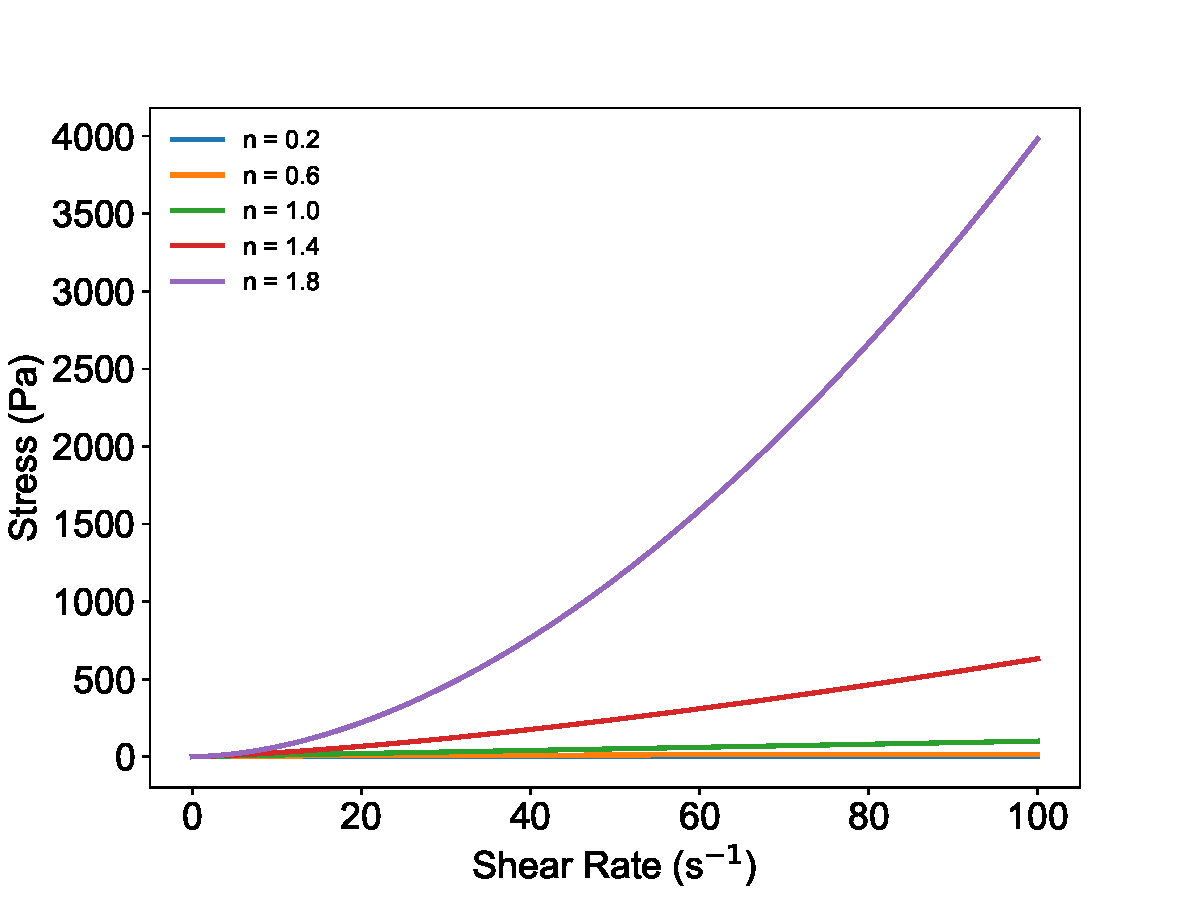
\includegraphics[width=0.8\textwidth]{Fig/herschel_moni.pdf}
  \FigureBicaption{\label{herschel_moni}Herschel-Bulkley模型模拟数据应力-应变率曲线图,n为流变指数}{Stress–strain rate curve of simulated data for the Herschel-Bulkley model, where n represents the flow index}
\end{figure}
本节使用Herschel-Bulkley模型模拟数据,模拟结果如图\ref{herschel_moni}所示。由图\ref{herschel_moni}可以看到,模拟数据中剪切应力(Stress)与剪切速率(Shear Rate)呈现幂函数关系,随着流变指数$n$的增加,曲线的斜率增大,表明流体的非牛顿特性增强。这一现象与Herschel-Bulkley模型的数学形式相符,说明模拟数据符合预期。
\subsubsection{GRU/DNN模型预测效果对比}

本节分别使用GRU和DNN两种算法对Herschel-Bulkley模型模拟数据进行深度学习建模,之后使用预测模型在测试集上进行验证,测试结果如图\ref{herschel_test}所示。图\ref{herschel_test}(a)为两种算法测试的真实值-预测值曲线,从曲线可以定性看出两种算法的预测值曲线与真实值曲线都非常接近。图\ref{herschel_test}(b)为两种算法测试结果的残差图,可以看出两种算法的残差点离散程度接近,均没有明显趋向性,均呈现无序分布,说明两种算法均可以比较好地捕捉到所有的输入特征。图\ref{herschel_test}(c-f)分别比较了两种算法预测结果的R$^2$,MAE,MAPE指标,从结果中可以看出,两种算法的预测效果都十分良好,R$^2$都接近1,GRU预测结果的R$^2$值略高于DNN,GRU预测结果的MAE和MAPE值都小于DNN,但数值差距不大。GRU算法的平均训练时间为378 s,高于DNN的155 s 一倍以上,这是由于GRU网络的参数量更大,且由于其循环神经网络的特点,只能顺序运算,限制了GPU的并行计算能力,导致训练时间较长。

综合看来GRU和DNN两种算法在Herschel-Bulkley模型模拟数据上的预测表现比较接近,从预测指标的绝对数值看,GRU略优于DNN。这个结果符合预期,因为Herschel-Bulkley模型本质上是模拟了剪切稀化增稠过程,不涉及黏弹性材料的时间依赖性,并且我们模拟的过程中,对于某个特定时间的应力状态也仅仅是当前应变状态的函数。从训练时间的分析看,GRU的训练成本远高于DNN。综合而言对于本构方程类似于Herschel-Bulkley模型的流体,GRU算法虽然在泛化效果上略有优势,但是综合性能上不具备显著优势。
\begin{figure}[H]
  \centering
  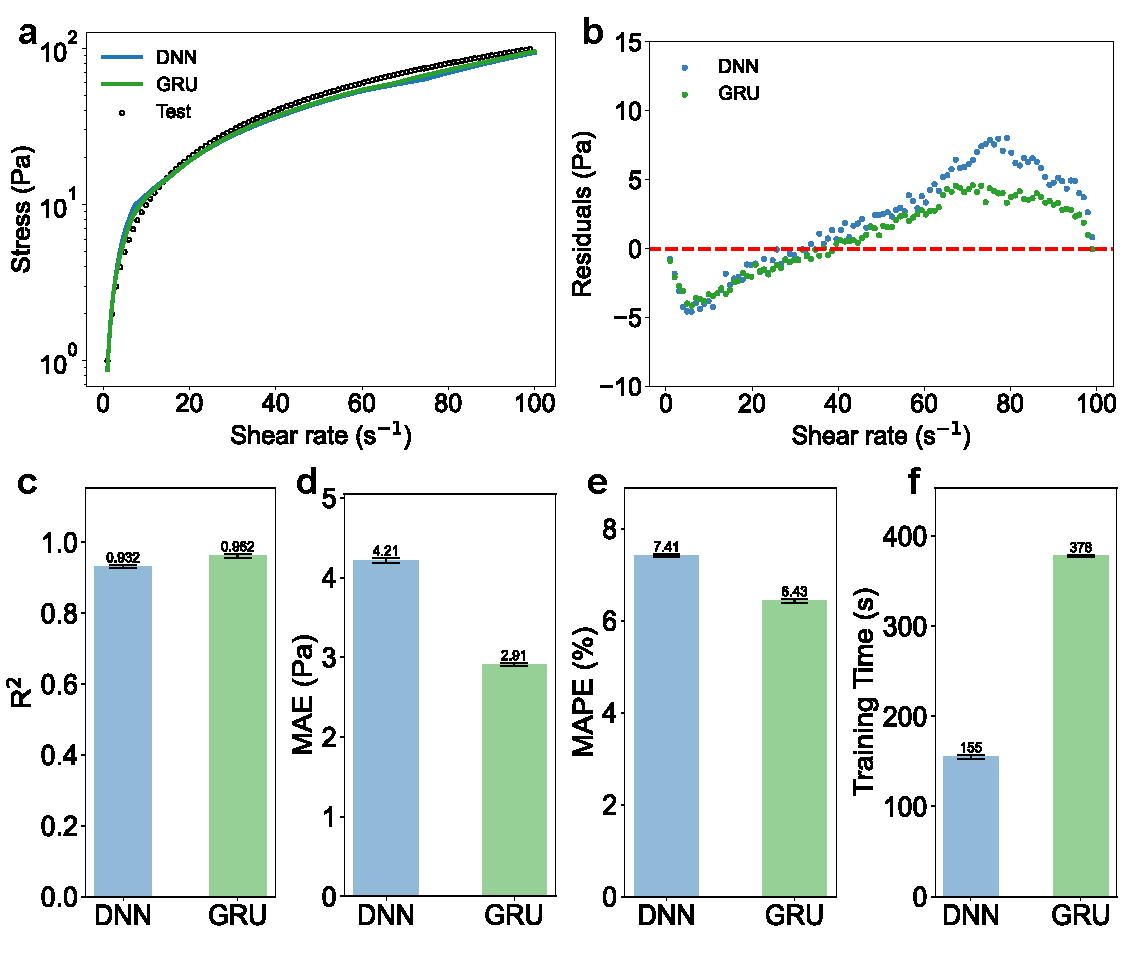
\includegraphics[width=0.8\textwidth]{Fig/Herschel_test.pdf}
  \FigureBicaption{\label{herschel_test}GRU算法和DNN算法在Herschel-Bulkley模型测试集上的预测效果对比示意图:(a)GRU和DNN在训练建模后的预测值-真实值曲线图;(b)GRU和DNN训练建模后的预测值残差图;(c)GRU和DNN测试集上的R$^2$指标图;(d)GRU和DNN在测试集上的MAE指标图;(e)GRU和DNN在测试集上的MAPE指标图;(f)GRU和DNN在测试集上的训练时间指标图}{Comparison schematic of the prediction performance of the GRU algorithm and the DNN algorithm on the Herschel-Bulkley model test set: (a) Predicted value–true value curves for GRU and DNN after training and modeling; (b) Residual plots of the predicted values for GRU and DNN after training and modeling; (c) R$^2$ metric plots on the test set for GRU and DNN; (d) MAE metric plots on the test set for GRU and DNN; (e) MAPE metric plots on the test set for GRU and DNN; (f) Training Time metric plots on the test set for GRU and DNN}
\end{figure}
\subsection{Maxwell模型建模}
\subsubsection{数值模拟数据}
\begin{figure}[htbp]
  \centering
  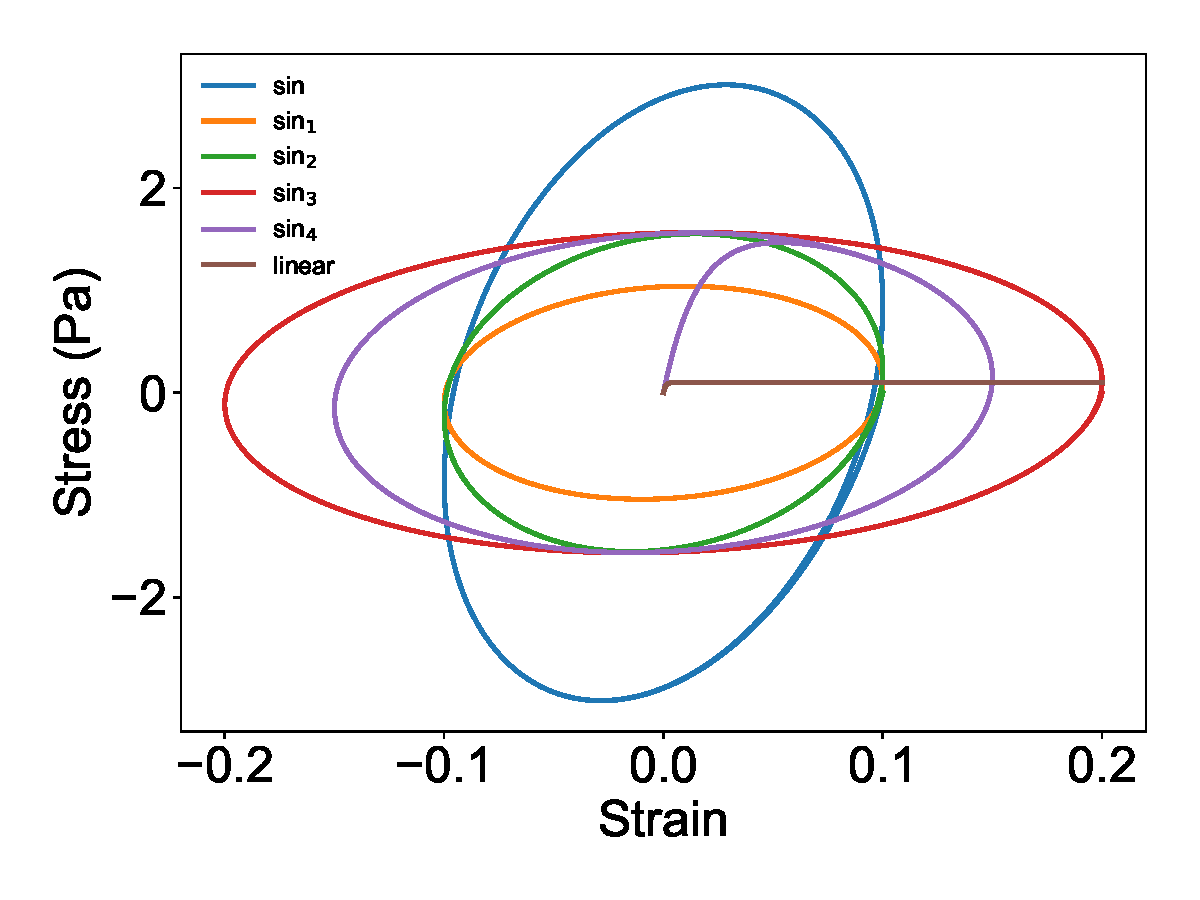
\includegraphics[width=0.8\textwidth]{Fig/maxwell_moni.pdf}
  \FigureBicaption{\label{maxwell_moni}不同应变变化协议的Maxwell模型模拟数据应力-应变曲线(Lissajous曲线)图}{Stress–strain curves (Lissajous curves) of simulated data for the Maxwell model under different strain variation protocols}
\end{figure}
本节通过后向欧拉法对简单 Maxwell 模型进行了数值模拟,生成了模拟数据,并绘制了应力-应变曲线(Lissajous 曲线),结果如图 \ref{maxwell_moni} 所示。图 \ref{maxwell_moni} 展示了不同应变协议下的模拟结果。对于正弦交变应变,Lissajous 曲线呈现出标准的闭合椭圆形状,这与 Maxwell 模型的理论预期一致,表明模型在周期性应变下的响应具有良好的稳定性和可预测性。对于线性应变,Lissajous 曲线在应变较小时表现出应力的快速增加,随后随着应变的继续增加,应力逐渐趋于一个稳定值,这一现象同样符合 Maxwell 模型的理论预期,反映了材料在持续应变下的应力松弛特性。综合看来,后向欧拉法模拟的数据符合预期,可以用于后续训练。


\subsubsection{交变协议预测交变协议效果验证}
\begin{figure}[htbp]
  \centering
  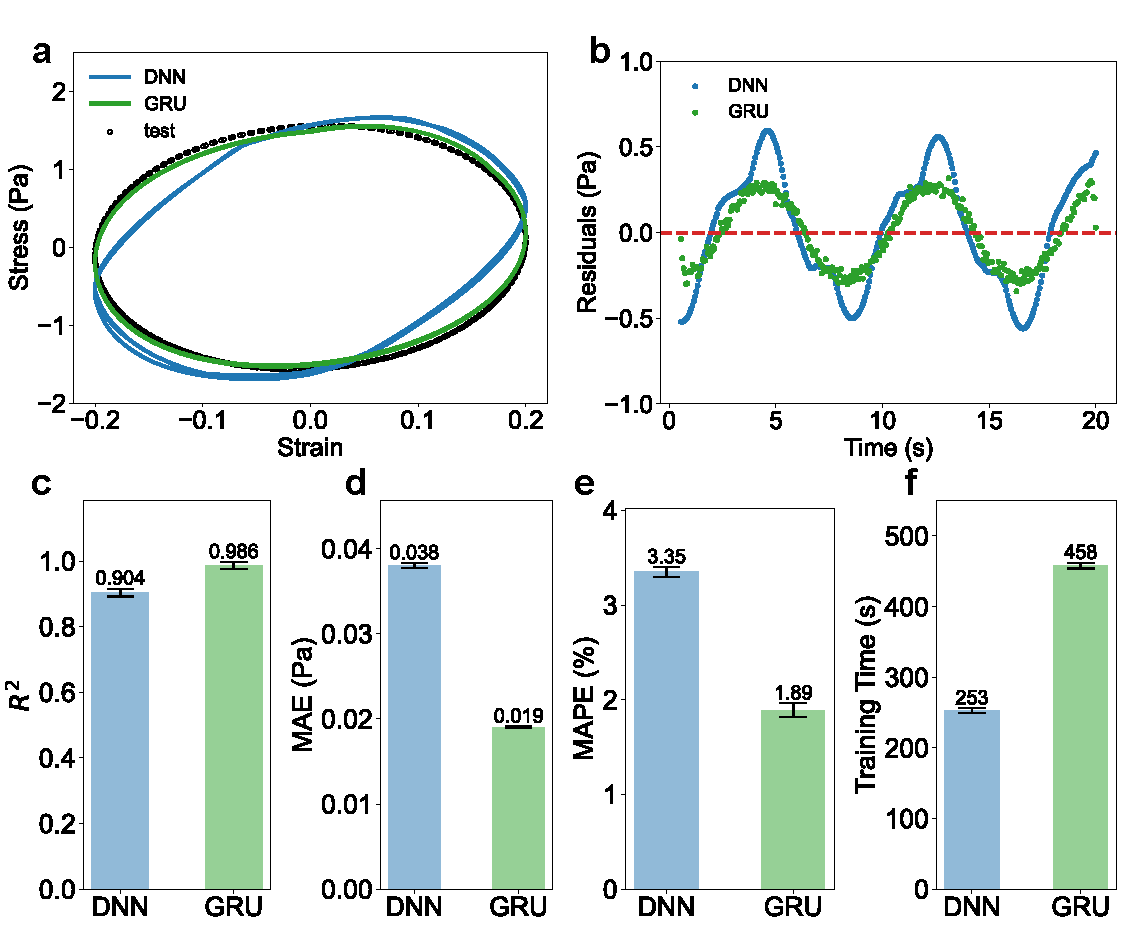
\includegraphics[width=0.8\textwidth]{Fig/Maxwell_sin_test.pdf}
  \FigureBicaption{\label{maxwell_sin}GRU算法和DNN算法在Maxwell模型交变协议测试集上的预测效果对比示意图:(a)GRU和DNN在测试集上的预测值与真实值的应力-应变曲线(Lissajous曲线);(b)GRU和DNN在测试集上的预测值与真实值的应力-时间曲线;(c)GRU和DNN在测试集上的预测值残差图}{Comparison of prediction performance between GRU and DNN algorithms on Maxwell model alternating protocol test set: (a) Stress-strain curves (Lissajous curves) of predicted vs. true values for GRU and DNN on test set; (b) Stress-time curves of predicted vs. true values for GRU and DNN on test set; (c) Residual plots of predicted values for GRU and DNN on test set}
\end{figure}
\begin{figure}[htbp]
  \centering
  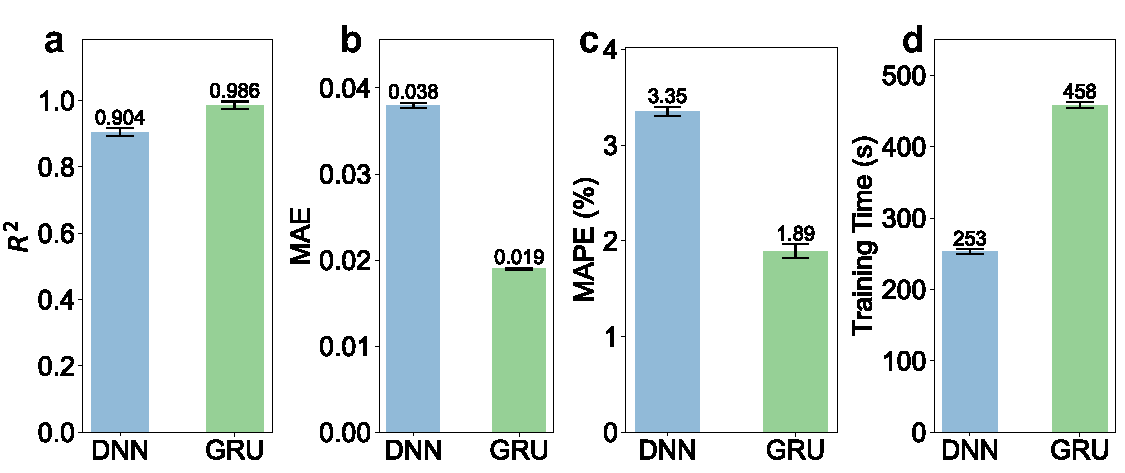
\includegraphics[width=0.8\textwidth]{Fig/Maxwell_sin_metric.pdf}
  \FigureBicaption{\label{maxwell_sin_metric}GRU算法和DNN算法在Maxwell模型交变测试集上的预测指标对比图:(a)GRU和DNN在测试集上的R$^2$指标图;(b)GRU和DNN在测试集上的MAE指标图;(c)GRU和DNN在测试集上的MAPE指标图;(d)GRU和DNN在测试集上的训练时间指标图}{Comparison schematic of the prediction performance of the GRU algorithm and the DNN algorithm on the Maxwell model alternating protocol test set: (a) R$^2$ metric plots on the test set for GRU and DNN; (b) MAE metric plots on the test set for GRU and DNN; (c) MAPE metric plots on the test set for GRU and DNN; (d) Training Time metric plots on the test set for GRU and DNN}
\end{figure}
为了验证GRU算法在时间序列本构方程数据中的预测效果,本节使用交变应变协议生成的数据作为训练集,交变应变协议生成的数据作为测试集。分别使用了GRU和DNN进行训练,并在测试集上进行验证,测试结果如图\ref{maxwell_sin}、图\ref{maxwell_sin_metric}所示。

图\ref{maxwell_sin}(a-b)为两种不同算法预测模型在测试集上的真实值-预测值曲线,
图a为Lissajous曲线,可以看到GRU算法的预测值的Lissajous曲线与真实值曲线十分接近,而DNN算法的预测值的Lissajous曲线与真实的曲线则有明显的周期性偏差,尤其在大应变时,预测值与真实值有较大的偏差。图b为时间-应力曲线,从中可以看到GRU算法的预测值曲线随时间变化较为稳定,贴近真实值曲线,而DNN算法的预测值的曲线明显偏离真实值曲线。

图\ref{maxwell_sin}(c)为两种算法预测模型的测试集残差图,从图中可以看到DNN算法的预测值与真实值残差呈现非常明显的周期性分布,极值偏离0刻度线,说明DNN模型无法泛化到测试集。而GRU的残差图虽然也存在一定周期性,但是总体分布效果明显优于DNN的对应残差,这说明GRU捕捉到了训练数据的较完整的特征,尤其是DNN未能捕捉的周期性特征。综合真实值-预测值曲线和残差图,可以定性分析出GRU的预测效果更为优秀。


接下来,本节计算两种算法的测试集预测指标,绘制指标对比图\ref{maxwell_sin_metric}。从图\ref{maxwell_sin_metric
}(a)显示,GRU的R$^2$值为0.986,接近1,说明GRU的预测效果十分优秀,而DNN的R$^2$值为0.904,略低于GRU,但是也高于0.9,属于非常出色的指标。仅从R$^2$指标来看,GRU预测效果优于DNN,但是优势不明显。从图\ref{maxwell_sin_metric}(b-c)看,GRU预测结果的MAE值为0.019,仅为DNN预测结果的MAE值的一半,GRU预测结果的MAPE值为1.89,仅为DNN预测结果的MAPE值3.35的一半。这定量说明GRU的预测结果误差远小于DNN的预测结果误差,GRU在此项任务上预测泛化效果更好。当然,由于GRU的模型特性,其训练时间如图\ref{maxwell_sin_metric}(d)所示,要高于DNN。

综合各项分析数据来看,当训练数据和测试数据为同类型应变变化过程(都为交变应变)时,GRU算法可以更好的学习到Maxwell模型数据的内在特征,包括周期性响应,黏弹性,时间依赖性响应。从定性与定量分析结果看,GRU算法的预测泛化效果在此项任务上明显优于DNN,在计算资源足够时,GRU算法相比DNN性能更佳。


\subsubsection{交变协议预测线性协议效果验证}
\begin{figure}[htbp]
  \centering
  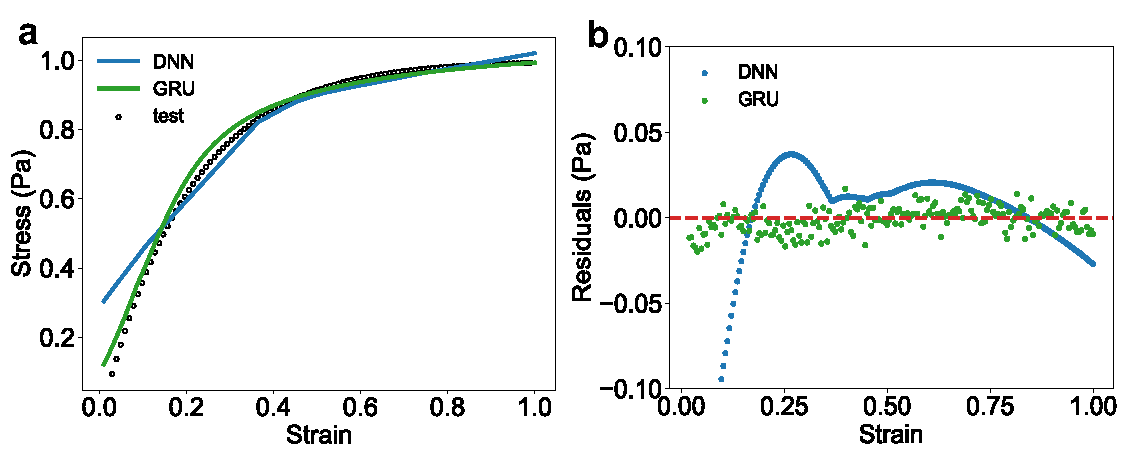
\includegraphics[width=0.8\textwidth]{Fig/maxwell_linear_test.pdf}
  \FigureBicaption{\label{maxwell_linear}GRU算法和DNN算法在Maxwell模型线性协议测试集上的预测效果对比示意图:(a)GRU和DNN在测试集上的预测值与真实值的应力-应变曲线(Lissajous曲线);(b)GRU和DNN在测试集上的预测值残差图}{Comparison of prediction performance between GRU and DNN algorithms on Maxwell model linear protocol test set: (a) Stress-strain curves (Lissajous curves) of predicted vs. true values for GRU and DNN on test set; (b) Residual plots of predicted values for GRU and DNN on test set}
\end{figure}
为了验证GRU算法在不同形式的应变历史下的泛化预测效果,本节使用交变应变协议生成的数据作为训练集,线性应变协议生成的数据作为测试集。分别使用了GRU和DNN进行训练,并在测试集上进行验证,测试结果如图\ref{maxwell_linear}、图\ref{maxwell_linear_metric}所示。
\begin{figure}[htbp]
  \centering
  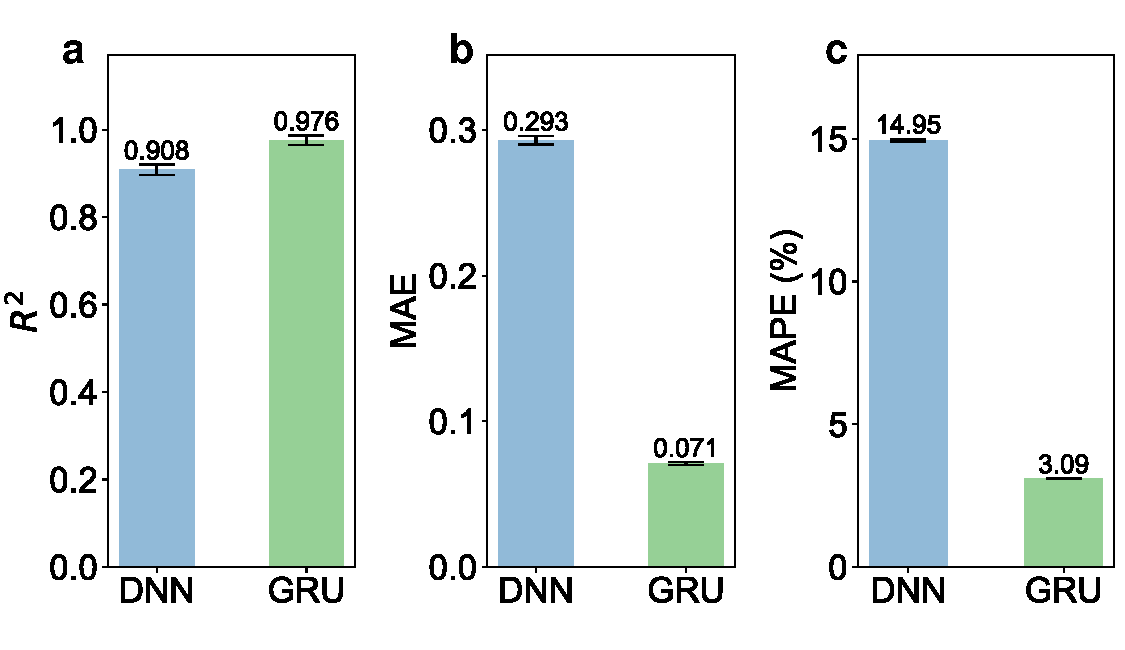
\includegraphics[width=0.8\textwidth]{Fig/maxwell_linear_metric.pdf}
  \FigureBicaption{\label{maxwell_linear_metric}GRU算法和DNN算法在Maxwell模型线性协议测试集上的预测指标对比图:(a)GRU和DNN在测试集上的R$^2$指标图;(b)GRU和DNN在测试集上的MAE指标图;(c)GRU和DNN在测试集上的MAPE指标图}{Comparison schematic of the prediction performance of the GRU algorithm and the DNN algorithm on the Maxwell model linear protocol test set: (a) R$^2$ metric plots on the test set for GRU and DNN; (b) MAE metric plots on the test set for GRU and DNN; (c) MAPE metric plots on the test set for GRU and DNN}
\end{figure}
图\ref{maxwell_linear}(a)为两种不同算法预测模型在测试集上的真实值-预测值的Lissajous曲线,图中可以看到GRU算法的预测值的Lissajous曲线与真实值曲线接近,在小应变时有一定偏差,这可能源于门控单元对初始状态记忆单元的权重初始化敏感性问题。而DNN算法的预测值的Lissajous曲线与真实的曲线相比GRU偏差更大,在小应变时,预测值与真实值有较大的偏差。

图\ref{maxwell_linear}(b)为两种算法预测模型的测试集残差图,从图中可以看到DNN算法的残差在初始时相比GRU更为偏离0刻度线,GRU的残差图残差点相对均匀地分布在0刻度线两侧,总体分布效果明显优于DNN的对应残差。这说明GRU捕捉到了训练数据的较完整的特征,且预测偏差较小。综合真实值-预测值曲线和残差图,可以定性分析出GRU的预测效果更为优秀。

接下来,本节计算两种算法的测试集预测指标,绘制指标对比图\ref{maxwell_linear_metric}。图\ref{maxwell_linear_metric}(a)显示,GRU的R$^2$值为0.976,接近1,证明GRU的预测效果十分优秀,而DNN的R$^2$值为0.908,略低于GRU,但是也高于0.9,属于非常出色的指标。仅从R$^2$指标来看,GRU预测效果优于DNN,但是优势不明显。从图\ref{maxwell_linear_metric}(b-c)看,GRU预测结果的MAE值为0.071,而DNN的预测结果的MAE值为0.293,GRU在绝对误差上仅为DNN的四分之一,优势显著。GRU预测结果的MAPE值为3.09,仅为DNN预测结果的MAPE值14.95的五分之一左右。这定量说明GRU的预测结果误差远小于DNN的预测结果误差,GRU在此项任务上预测泛化效果更好。这里的训练时间对比与上一节的交变协议预测交变协议一致,同图\ref{maxwell_sin_metric}(d)所示。


综合各项分析数据来看,当训练数据和测试数据为不同类型应变变化过程时,GRU算法展现出了显著的优势,尤其是在学习Maxwell模型数据的内在特征方面。Maxwell模型作为一种经典的粘弹性模型,其核心在于描述材料在应力作用下的时间依赖性响应。GRU算法可以仅通过学习交变应变的训练数据,就能够很好地预测线性应变的测试数据。这是因为GRU算法能够有效地从交变应变数据中提取出关键的时间依赖性特征,并将其应用于线性应变的预测中。
\subsubsection{不同时间步的预测效果对比}
\begin{figure}[htbp]
  \centering
  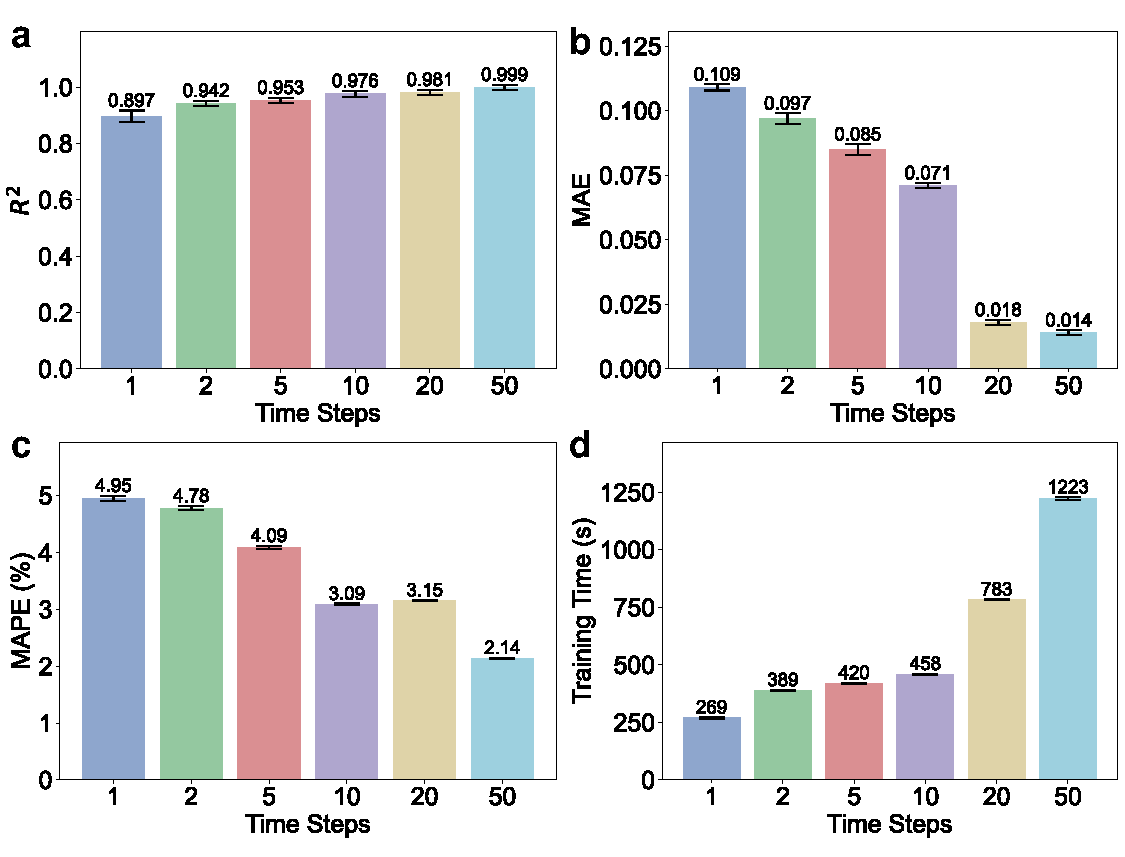
\includegraphics[width=0.8\textwidth]{Fig/Maxwell_timesteps_metrics.pdf}
  \FigureBicaption{\label{maxwell_timesteps_metrics}GRU算法在Maxwell模型不同时间步下的预测效果对比图:(a)GRU在不同时间步下的R$^2$指标图;(b)GRU在不同时间步下的MAE指标图;(c)GRU在不同时间步下的MAPE指标图;(d)GRU在不同时间步下的训练时间指标图}{Comparison of prediction performance of the GRU algorithm on the Maxwell model with different time steps: (a) R$^2$ metric plots with different time steps; (b) MAE metric plots with different time steps; (c) MAPE metric plots with different time steps; (d) Training Time metric plots with different time steps}
\end{figure}
对于GRU这类循环神经网络来说,网络架构的时间步数(序列长度)是非常重要的超参数。较大的时间步可以使模型在每个时间步上处理更多的信息,有助于捕捉长期依赖关系,但是可能导致模型学习到数据中的噪声,而不是其潜在的结构,从而导致过拟合。较小的时间步较小的时间步可以更细致地捕捉序列中的短期变化和细节信息,有助于模型更好地理解数据的短期动态特征,可能导致模型过于关注噪声,而忽略重要的长期依赖关系,从而导致欠拟合。本节研究了不同时间步下训练的模型在测试集上的预测效果。如图\ref{maxwell_timesteps_metrics}所示。由图可见,预测模型R$^2$值随着时间步的增加而增加,但是幅度较小。MAE值和MAPE值随时间步的增加而减少,说明随着时间步的增加,模型的预测效果变的更好,时间步小于10时,这种误差减小的趋势较明显,时间步大于20时,MAE值下降幅度变小,时间步大于10,MAPE值下降幅度变小。这说明模型的优化指标上升存在阈值,这是因为GRU算法在较长序列中容易遗忘丢失信息,对于时间序列的处理长度有一定限制。而随着时间步的增加,当时间步大于20后,模型的训练时间急剧增加,训练成本陡增。

本节分析针对此项任务,最佳时间步在10-20之间,MAE值和MAPE值开始下降到阈值,且训练时间还未显著增加。


% Doi-Edwards模型建模
\subsection{Doi-Edwards模型建模}
\subsubsection{数值模拟数据}
\begin{figure}[htbp]
  \centering
  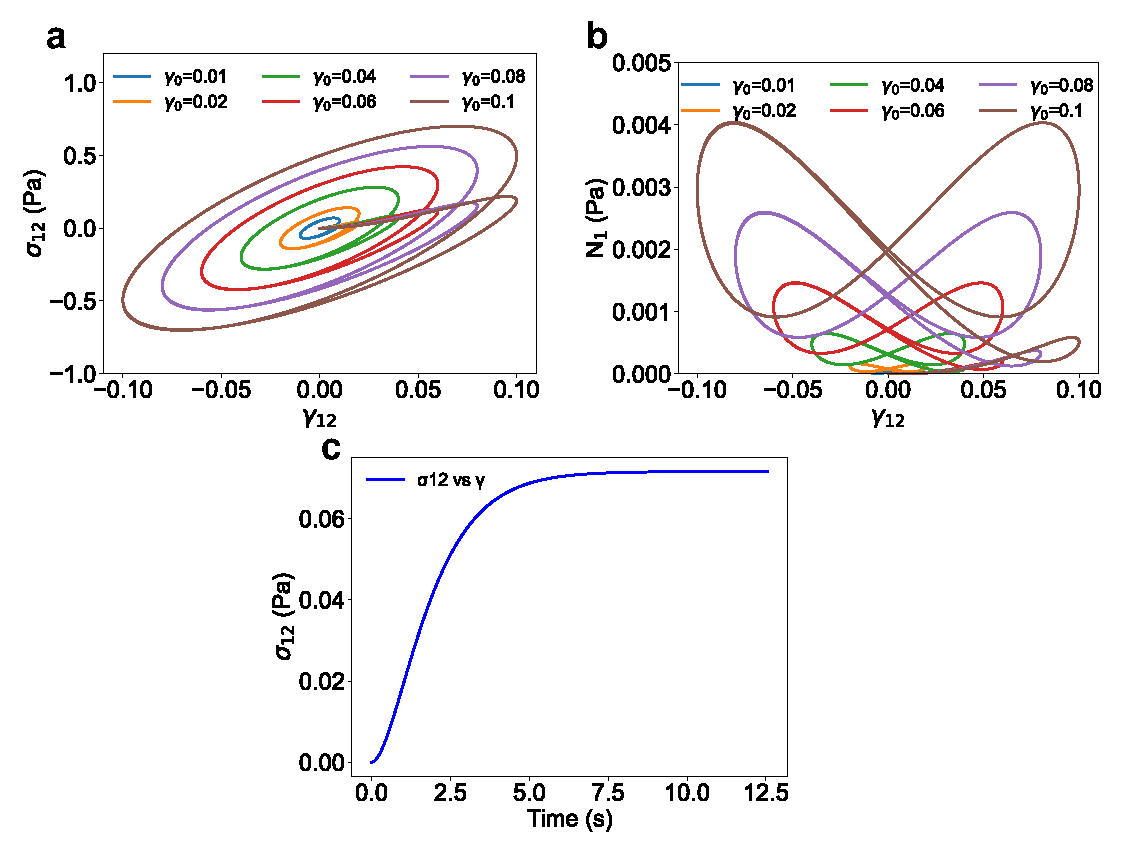
\includegraphics[width=0.8\textwidth]{Fig/doi-edwards-moni.pdf}
  \FigureBicaption{\label{doi-edwards-moni}Doi-Edwards模型模拟数据:(a)不同应变振幅下的剪切应力应变Lissajous曲线;(b)不同应变振幅下的第一法向应力差(N$_1$)的Lissajous曲线;(c)线性应变协议下的应力-时间曲线}{Doi-Edwards model simulation data: (a) Lissajous curves of shear stress-strain under different strain amplitudes; (b) Lissajous curves of first normal stress difference (N$_1$); (c) Stress-time curves under linear strain protocol}
\end{figure}
本节使用Python的scipy.integrate库对Doi-Edwards模型进行数值积分模拟。模拟结果如图\ref{doi-edwards-moni}所示。图\ref{doi-edwards-moni}(a)为不同应变振幅模拟的剪切应力应变Lissajous曲线,曲线呈现标准的椭圆形状,符合Doi-Edwards模型在小应变下的假设。图\ref{doi-edwards-moni}(b)为模拟的第一法向应力差(N$_1$)的Lissajous曲线,曲线具有振幅依赖性,且为滞回曲线,与文献中的Doi-Edwards模型一致。图\ref{doi-edwards-moni}(c)为线性应变协议下的应力-时间曲线,可以看到随着应变加载,应力一开始为近似的线性增加,后逐渐趋向平台值,这个结果符合预期。综上本节模拟的数据可以认为符合Doi-Edwards模型,可以用于后续实验。

\subsubsection{交变协议预测交变协议效果验证}
\begin{figure}[htbp]
  \centering
  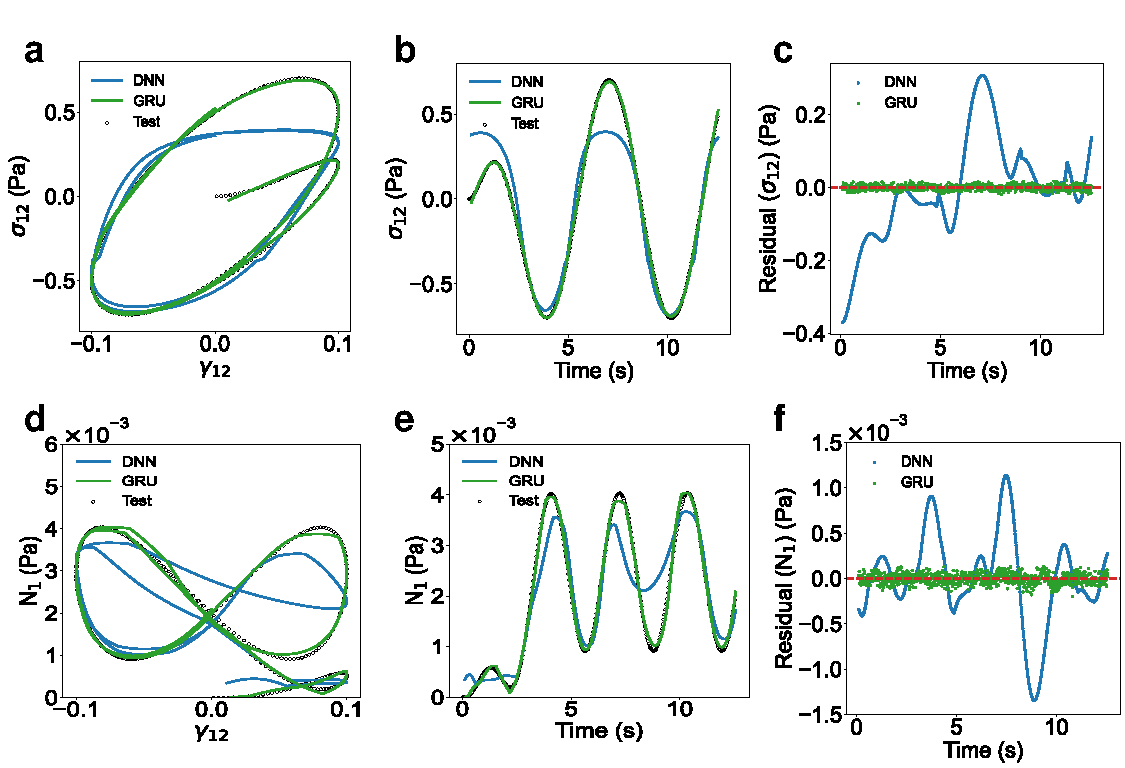
\includegraphics[width=0.8\textwidth]{Fig/doi-edwards-sin.pdf}
  \FigureBicaption{\label{doi-edwards-sin}GRU算法和DNN算法在Doi-Edwards模型交变协议测试集上的预测效果对比示意图:(a)GRU和DNN在测试集上的预测值与真实值的剪切应力-应变曲线(Lissajous曲线);(b)GRU和DNN在测试集上的预测值与真实值的时间-应力曲线;(c)GRU和DNN在测试集上剪切应力的预测值残差图;(d)GRU和DNN在测试集上的预测值与真实值的第一法向应力差(N$_1$)的Lissajous曲线;(e)GRU和DNN在测试集上的预测值与真实值的时间-第一法向应力差曲线;(f)GRU和DNN在测试集上的第一法向应力差预测值残差图}{Comparison schematic of the prediction performance of the GRU algorithm and the DNN algorithm on the Doi-Edwards model alternating protocol test set: (a) Shear stress-strain curves (Lissajous curves) of predicted vs. true values for GRU and DNN on test set; (b) Time-stress curves of predicted vs. true values for GRU and DNN on test set; (c) Residual plots of shear stress predicted values for GRU and DNN on test set; (d) First normal stress difference (N$_1$) Lissajous curves of predicted vs. true values for GRU and DNN on test set; (e) Time-first normal stress difference curves of predicted vs. true values for GRU and DNN on test set; (f) Residual plots of first normal stress difference predicted values for GRU and DNN on test set}
\end{figure}
\begin{figure}[htbp]
  \centering
  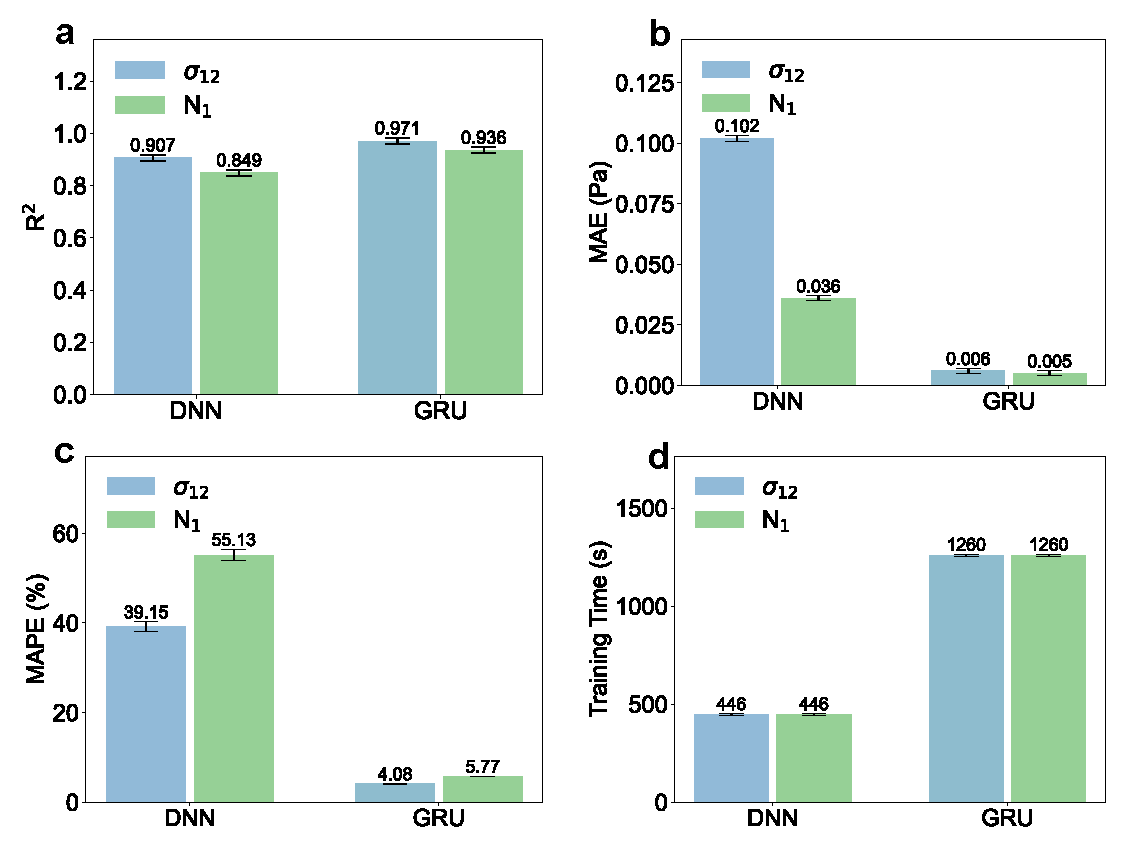
\includegraphics[width=0.8\textwidth]{Fig/doi-edwards-sin-metrics.pdf}
  \FigureBicaption{\label{doi-edwards-sin-metric}GRU算法和DNN算法在Doi-Edwards模型交变协议测试集上的预测指标对比图:(a)GRU和DNN在测试集上的R$^2$指标图;(b)GRU和DNN在测试集上的MAE指标图;(c)GRU和DNN在测试集上的MAPE指标图;(d)GRU和DNN在测试集上的训练时间指标图}{Comparison schematic of the prediction performance of the GRU algorithm and the DNN algorithm on the Doi-Edwards model alternating protocol test set: (a) R$^2$ metric plots on the test set for GRU and DNN; (b) MAE metric plots on the test set for GRU and DNN; (c) MAPE metric plots on the test set for GRU and DNN; (d) Training Time metric plots on the test set for GRU and DNN}
\end{figure}
为了验证GRU算法在Doi-Edwards模型本构方程数据中的预测效果,本节使用交变应变协议生成的数据作为训练集,交变应变协议生成的数据作为测试集。分别使用了GRU和DNN进行训练,并在测试集上进行验证,测试结果如图\ref{doi-edwards-sin}、图\ref{doi-edwards-sin-metric}所示。

图\ref{doi-edwards-sin}(a-c)为两种不同算法构建的预测模型预测的剪切应力($\sigma_{12}$)的Lissajous曲线、时间-应力曲线、残差图,(d-f)为预测的第一法向应力差(N$_{1}$)的Lissajous曲线、时间-应力曲线、残差图。
图a和图b可以看出GRU算法的预测的$\sigma_{12}$值与真实的$\sigma_{12}$接近,曲线拟合较好。而DNN算法的预测值在某些区域存在较大误差,例如在应变变化的初始和5-10 s之间,DNN存在较大误差。图c的残差图则显示,GRU算法预测值与真实值的残差紧贴0刻度线,呈现无序离散的分布状态,而DNN算法预测值和真实值的残差呈现明显的曲线规律,且与0刻度线性距离偏差较大,残差分布区间远远大于GRU部分。残差图的结果表明对于GRU成功地学习到了训练数据中的各项特征,复杂的非线性关系,且不存在明显周期性,总体残差较小,而DNN存在特征未能完全学习的问题,拟合效果较差,未能很好地捕捉到训练数据的特征。从图d、图e和图f的N$_1$的预测效果图来看,N$_1$与$\sigma_{12}$的结果类似,均是GRU的预测效果要由于DNN,而对比GRU预测的N$_1$值和$\sigma_{12}$值,则是$\sigma_{12}$值的预测效果会更好,这可能是因为$\sigma_{12}$与输入的剪切速率特征$\dot{\gamma_{12}}$之间的函数关系更为简单,且更加符合时间叠加原理,所以GRU可以更好地捕捉其时间依赖性和内在联系。


之后本节分别对两种不同算法在$\sigma_{12}$和N$_1$上的预测效果做了定量分析,指标图如图\ref{doi-edwards-sin-metric}所示。在R$^2$指标上,GRU在$\sigma_{12}$和N$_1$的预测指标均优于DNN,而同种算法下$\sigma_{12}$的R$^2$值要高于N$_1$,显示$\sigma_{12}$的预测效果更好。在MAE指标上,DNN的$\sigma_{12}$和N$_1$的MAE值均远高于GRU,说明GRU的预测误差远小于DNN。MAPE指标与MAE指标的对比基本一致,都是GRU的预测误差小于DNN。但是同种算法下$\sigma_{12}$的MAE值高于N$_1$,但是MAPE值反之,这是因为MAE值强调的是绝对值比较,受到真实数据本身尺度的影响,因此比较同种算法下$\sigma_{12}$和N$_1$的预测效果应当以去除了数据尺度影响的MAPE值来判定,而MAPE值的结论表明同种算法下$\sigma_{12}$值的预测效果相比N$_1$更好,这与R$^2$的分析和图\ref{doi-edwards-sin}的定性分析一致,这也是后续可以优化的方向之一。最后,从图\ref{doi-edwards-sin-metric}(d)来看,GRU在此项任务上的训练时间为DNN的3倍左右,符合更高成本的预期。

综合各项分析数据来看,当训练数据和测试数据为同类型应变变化过程(都为交变应变)时,GRU算法可以更好的学习到Doi-Edwards模型数据的内在特征,包括周期性响应,黏弹性,时间依赖性响应。从定性与定量分析结果看,GRU算法的预测泛化效果在此项任务上明显优于DNN,在计算资源足够时,GRU算法相比DNN性能更佳,而在同种算法下$\sigma_{12}$的预测效果优于N$_1$。
\subsubsection{交变协议预测线性协议效果验证}
\begin{figure}[htbp]
  \centering
  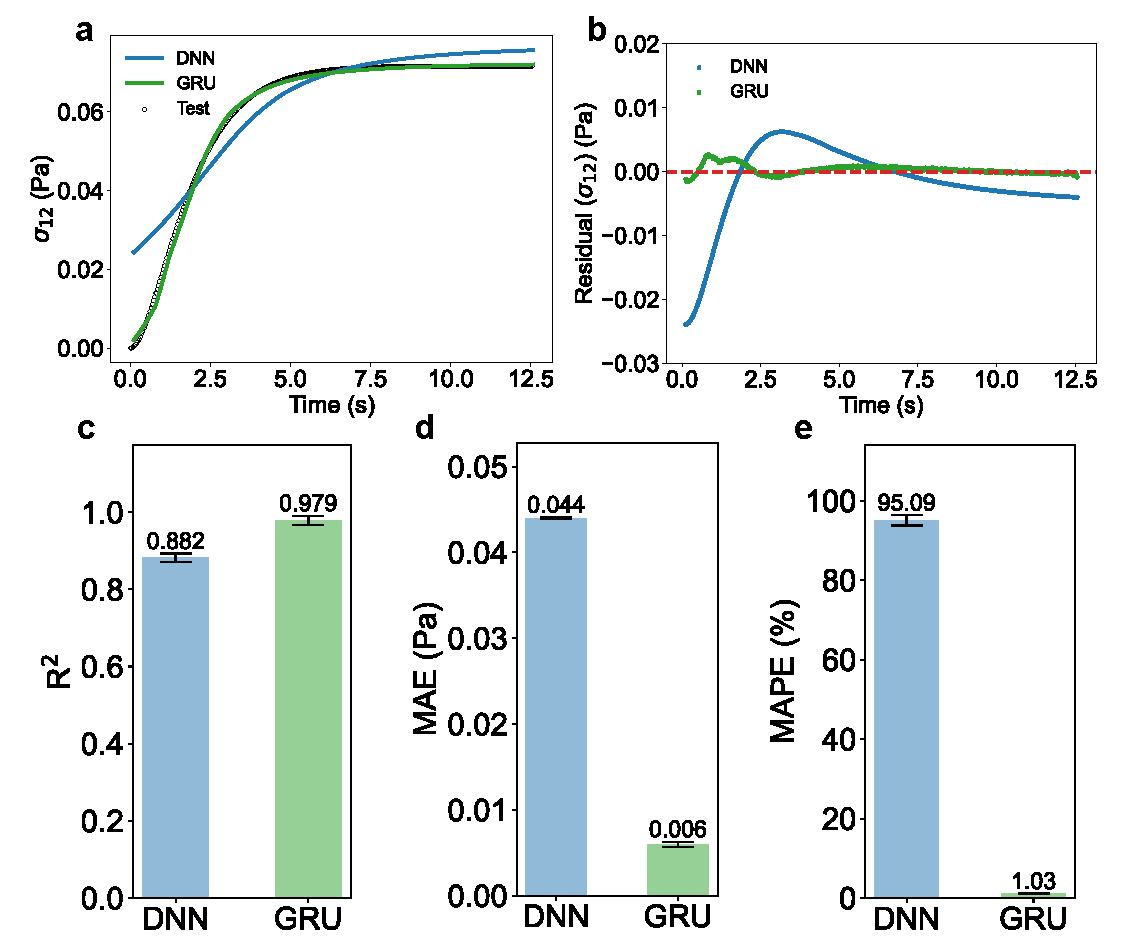
\includegraphics[width=0.8\textwidth]{Fig/doi-edwards-linear.pdf}
  \FigureBicaption{\label{doi-edwards-linear}GRU算法和DNN算法在Doi-Edwards模型线性协议测试集上的预测效果对比示意图:(a)GRU和DNN在测试集上的预测值与真实值的剪切应力-应变曲线(Lissajous曲线);(b)GRU和DNN在测试集上的预测值残差图}{Comparison schematic of the prediction performance of the GRU algorithm and the DNN algorithm on the Doi-Edwards model linear protocol test set: (a) Shear stress-strain curves (Lissajous curves) of predicted vs. true values for GRU and DNN on test set; (b) Residual plots of predicted values for GRU and DNN on test set}
\end{figure}
\begin{figure}[htbp]
  \centering
  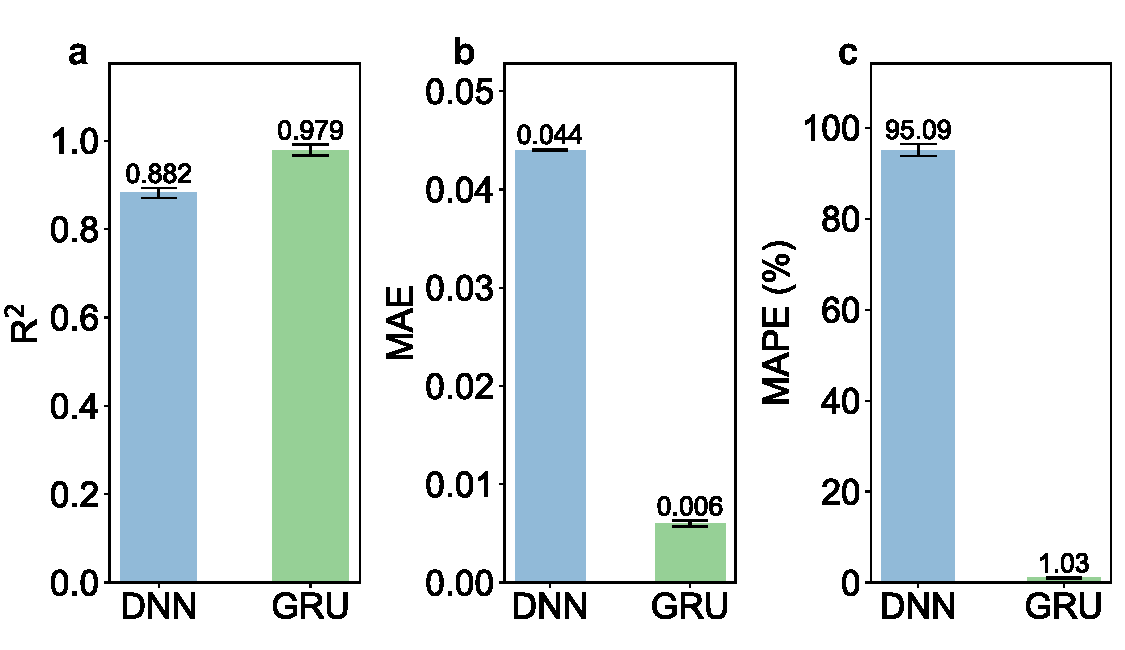
\includegraphics[width=0.8\textwidth]{Fig/doi-edwards-linear-metrics.pdf}
  \FigureBicaption{\label{doi-edwards-linear-metrics}GRU算法和DNN算法在Doi-Edwards模型线性协议测试集上的预测效果对比示意图:(a)GRU和DNN在测试集上的R$^2$指标图;(b)GRU和DNN在测试集上的MAE指标图;(c)GRU和DNN在测试集上的MAPE指标图}{Comparison schematic of the prediction performance of the GRU algorithm and the DNN algorithm on the Doi-Edwards model linear protocol test set: (a) R$^2$ metric plots on the test set for GRU and DNN; (b) MAE metric plots on the test set for GRU and DNN; (c) MAPE metric plots on the test set for GRU and DNN}
\end{figure}
为了验证GRU算法在不同形式的应变历史下对于Doi-Edwards模型泛化预测效果,本节使用交变应变协议生成的数据作为训练集,线性应变协议生成的数据作为测试集。分别使用了GRU和DNN进行训练,并在测试集上进行验证,测试结果如图\ref{doi-edwards-linear}、图\ref{doi-edwards-linear-metrics}所示。

图\ref{doi-edwards-linear}(a)为两种不同算法预测模型在测试集上的真实值-预测值曲线,图中可以看到GRU算法的预测值的曲线与真实值曲线接近,无较明显的偏差区间,而DNN算法的预测值的曲线与真实的曲线存在明显的偏差。在应变加载初始和结束时,DNN算法的预测值相比真实值偏大,而应变加载2-6 s的中间阶段,DNN算法的预测值又偏小,总体来看仅在大致趋势上符合真实值曲线。

图\ref{doi-edwards-linear}(b)展示了两种算法在测试集上的残差图。从图中可以明显看出,DNN算法的预测值与真实值之间的残差分布并不均匀,整体呈现出较为清晰的曲线趋势,尤其是在3秒附近出现了显著的峰值。这表明DNN未能充分捕捉到训练数据中的关键特征,导致其在测试集上的表现不尽如人意。相比之下,GRU算法的残差图则呈现出无序分布,残差点均匀地分布在0刻度线两侧,且残差值普遍小于DNN。这说明GRU能够更好地捕捉到训练数据中的特征,预测偏差也更小。综合真实值与预测值的曲线以及残差图的分析,可以定性地得出结论:GRU的预测效果优于DNN。

接下来,本节对两种算法在测试集上的预测性能指标进行了详细计算,并绘制了相应的指标对比图,如图\ref{doi-edwards-linear-metrics}所示。从图\ref{doi-edwards-linear-metrics}(a)中可以看出,GRU算法的 R$^2$值达到了0.979,这一结果充分证明了GRU在预测任务中的卓越表现。相比之下,DNN算法的 R$^2$值仅为0.882,明显低于GRU,这表明在 R$^2$指标的评估中,GRU的表现更为出色。进一步观察图\ref{doi-edwards-linear-metrics}(b-c),可以发现GRU预测结果的平均绝对误差(MAE)值为0.006,而DNN的MAE值则高达0.044。这意味着GRU在绝对误差方面的表现仅为DNN的七分之一,优势极为显著。此外,GRU预测结果的平均绝对百分比误差(MAPE)值为1.03,而DNN的MAPE值则为95.09。这些定量数据充分说明了GRU的预测结果误差远小于DNN,从而证明了GRU在该任务上的预测泛化能力更强。
至于训练时间的对比,与上一节中交变协议预测交变协议的情况一致,具体可参考图\ref{doi-edwards-sin-metric}(d)所示。

从整体分析数据来看,当训练数据与测试数据涉及不同类型的应变变化过程时,GRU算法在学习Doi-Edwards模型数据的内在特性方面有显著优势。这主要归因于GRU算法能够高效地从交变应变数据中提取关键的时间依赖特征,并将其成功应用于线性应变的预测之中。

\subsubsection{不同时间步的预测效果对比}

为了探究在Doi-Edwards模型上GRU算法的最佳时间步,本节研究了不同时间步下训练的模型在测试集上的预测效果,如图\ref{doi-edwards-timesteps-metrics}所示。由图可见,预测模型R$^2$值在时间步小于40时随着时间步的增加而增加,在时间步大于40后反而略有下降。MAE值和MAPE值在时间步小于40时随时间步的增加而减少,时间步为40的值只有不到时间步为20的值的十分之一,显著下降,而时间步大于40后,MAE值和MAPE值则趋于稳定。这说明对于本项任务,时间步为40左右时,恰好可以开始获得不错的预测效果,而从训练成本来看,训练时间是随着时间步设置增加而单调增的,所以综合看来,时间步为40左右时,性价比最高。
\begin{figure}[H]
  \centering
  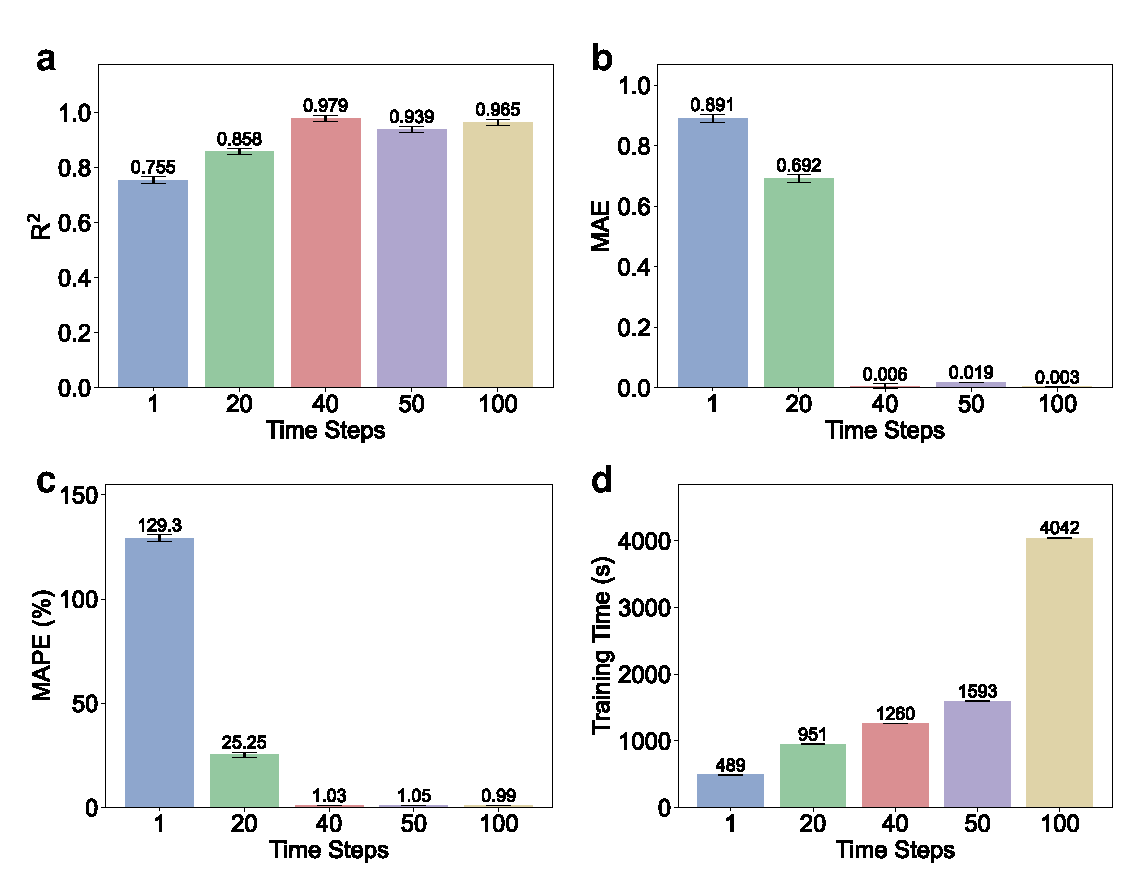
\includegraphics[width=0.8\textwidth]{Fig/doi-edwards-timesteps-metrics.pdf}
  \FigureBicaption{\label{doi-edwards-timesteps-metrics}GRU算法和DNN算法在Doi-Edwards模型不同时间步长下的预测指标对比图:(a)GRU和DNN在不同时间步下的R$^2$指标图;(b)GRU和DNN在不同时间步下的MAE指标图;(c)GRU和DNN在不同时间步下的MAPE指标图;(d)GRU和DNN在不同时间步下的训练时间指标图}{Comparison schematic of the prediction performance of the GRU algorithm and the DNN algorithm under different time steps of the Doi-Edwards model: (a) R$^2$ metric plots under different time steps for GRU and DNN; (b) MAE metric plots under different time steps for GRU and DNN; (c) MAPE metric plots under different time steps for GRU and DNN; (d) Training Time metric plots under different time steps for GRU and DNN}
\end{figure}
% Giesekus模型建模
\subsection{Giesekus模型建模}
\subsubsection{数值模拟数据}
\begin{figure}[htbp]
  \centering
  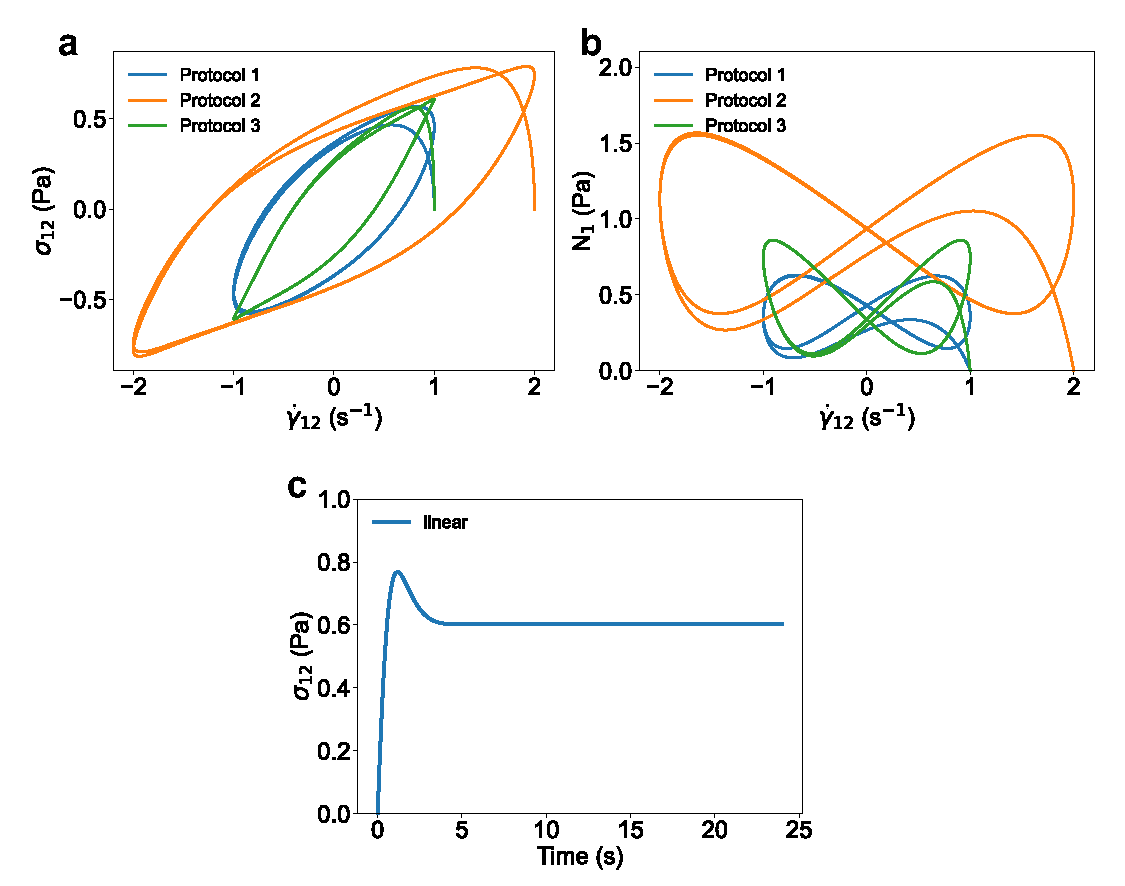
\includegraphics[width=0.8\textwidth]{Fig/giesekus-moni.pdf}
  \FigureBicaption{\label{giesekus_moni}Giesekus模型模拟数据:(a)不同交变应变协议的应力-应变率Lissajous曲线;(b)不同交变应变协议的第一法向应力差-应变率Lissajous曲线;(c)线性应变协议下的应力-时间曲线}{Giesekus model simulation data: (a) Lissajous curves of stress-strain rate for different oscillatory shear protocols; (b) Lissajous curves of first normal stress difference-strain rate for different oscillatory shear protocols; (c) Stress-time curve under linear strain protocol}
\end{figure}
本节通过Python的微分方程求解库来模拟Giesekus模型,模拟结果如图\ref{giesekus_moni}。

图\ref{giesekus_moni}展示了部分模拟数据,主要展示不同应变振幅下,本构关系从线性本构到非线性的转变。图\ref{giesekus_moni}(a)展示了不同交变应变协议的应力-应变率Lissajous曲线,Protocol 1为小振幅振荡剪切(SAOS)的模拟曲线,呈现椭圆状的滞后环,随着振幅增加,Protocol 2和 Protocol 3呈现非线性特征的扭曲和不对称,这是大振幅振荡剪切(LAOS)的拟合曲线。图\ref{giesekus_moni}(b)展示了不同交变应变协议的第一法向应力差(N$_1$)-应变率Lissajous曲线,随着振幅增加呈现不对称扭曲,曲线形状符合Giesekus模型假设\cite{lennonScientificMachineLearning2023a}。

图\ref{giesekus_moni}(c)为线性应变协议下的应力-时间曲线,曲线先随着应变加载攀升,存在明显峰值后回落,后趋于稳定。这可能是因为在屈服点之前,材料主要表现出弹性行为,应力随着应变的增加而线性增长。当应力达到峰值时,材料开始发生塑性变形,内部结构发生不可逆的变化,峰值之后,材料的内部结构开始重新组织,形成新的平衡状态,这种重组过程通常伴随着应力的下降与重新平衡。综上,线性协议的曲线符合Giesekus模型对于大剪切应变下材料应力响应的假设,可以用于后续实验。

\subsubsection{交变协议预测交变协议效果验证}
为了评估 GRU 算法在 Giesekus 模型本构方程数据预测中的有效性,本节采用交变应变协议生成的数据作为训练集与测试集,分别运用 GRU 和 DNN 进行模型训练,并在测试集上开展验证工作,测试结果如图 \ref{giesekus_sin}、图 \ref{giesekus-sin-metrics} 所示。

图 \ref{giesekus_sin}(a-c)分别为两种算法构建的预测模型所预测的剪切应力($\sigma_{12}$)的 Lissajous 曲线、时间-应力曲线以及残差图,(d- f)则对应预测的第一法向应力差(N$_{1}$)的Lissajous曲线、时间- 应力曲线与残差图。

从图a和图b可以观察到,GRU算法预测的$\sigma_{12}$值与真实值高度接近,曲线拟合效果理想,而DNN算法在部分区域的预测值存在较大偏差。图 c 的残差图进一步显示,GRU算法预测值与真实值的残差紧密围绕 0 刻度线,呈无序离散分布;相比之下,DNN算法预测值与真实值的残差呈现出明显的曲线规律及周期性特征,且与0刻度线的偏离程度较大,残差分布区间显著宽于GRU部分。残差图的结果有力地表明,GRU成功地学习到了训练数据中的各类特征及复杂的非线性关系,不存在明显的周期性规律,整体残差较小;而DNN存在未能充分学习特征的问题,拟合效果欠佳,未能精准捕捉训练数据的特征。

对于图d、图e和图f所展示的N$_{1}$预测效果,其与$\sigma_{12}$的结果呈现出相似性,即GRU的预测性能优于DNN。进一步对比GRU预测的N$_{1}$值和 $\sigma_{12}$值,发现$\sigma_{12}$值的预测效果更为优异,这可能归因于 $\sigma_{12}$与输入的剪切速率特征 $\dot{\gamma_{12}}$ 之间的函数关系相对简单,且更契合时间叠加原理,从而使得GRU能够更有效地捕捉其时间依赖性及内在联系。这部分的模型结果与Doi-Edwards模型结果类似,对于第一法向应力差(N$_1$),目前的GRU模型存在进一步改进的空间。
\begin{figure}[htbp]
  \centering
  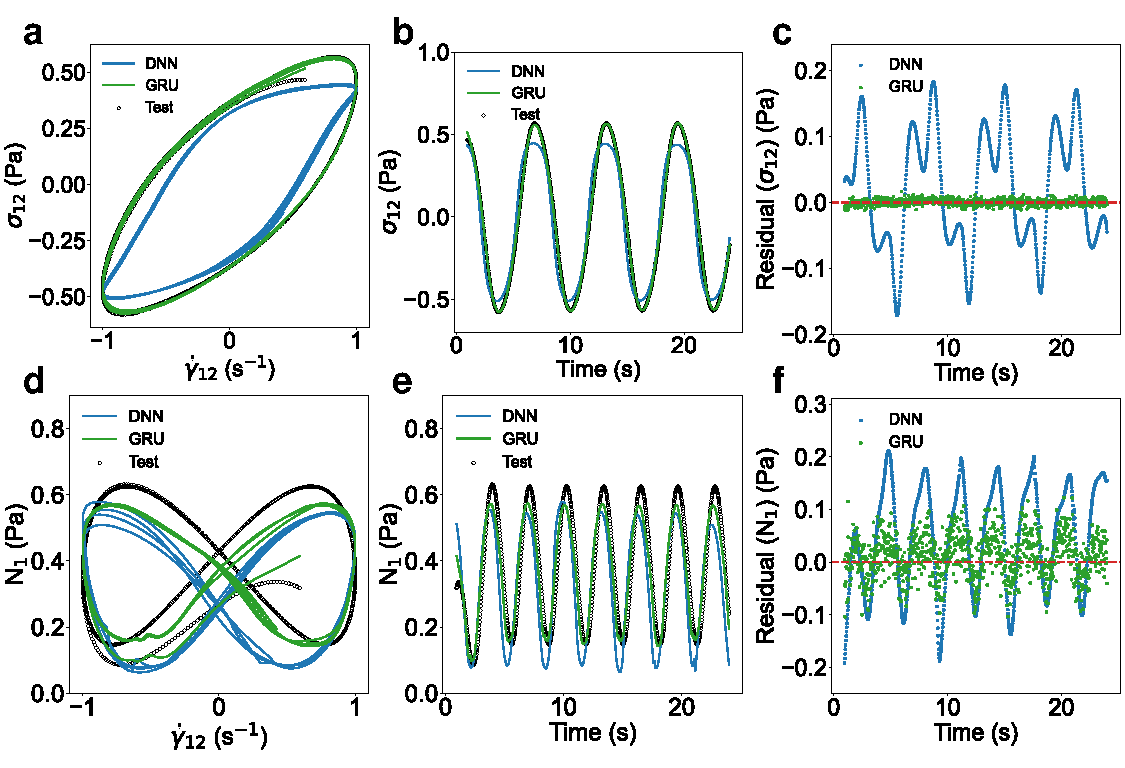
\includegraphics[width=0.8\textwidth]{Fig/giesekus_sin.pdf}
  \FigureBicaption{\label{giesekus_sin}GRU算法和DNN算法在Giesekus模型交变协议测试集上的预测效果对比示意图:(a)GRU和DNN在测试集上的预测值与真实值的剪切应力-应变率Lissajous曲线;(b)GRU和DNN在测试集上的剪切应力-时间曲线;(c)GRU和DNN在测试集上的剪切应力预测值残差图;(d)GRU和DNN在测试集上的预测值与真实值的第一法向应力差-应变率Lissajous曲线;(e)GRU和DNN在测试集上的第一法向应力差-时间曲线;(f)GRU和DNN在测试集上的第一法向应力差预测值残差图}{Comparison schematic of the prediction performance of the GRU algorithm and the DNN algorithm on the Giesekus model oscillatory protocol test set: (a) Shear stress-strain rate Lissajous curves of predicted vs. true values for GRU and DNN on test set; (b) Shear stress-time curves for GRU and DNN on test set; (c) Residual plots of shear stress predicted values for GRU and DNN on test set; (d) First normal stress difference-strain rate Lissajous curves of predicted vs. true values for GRU and DNN on test set; (e) First normal stress difference-time curves for GRU and DNN on test set; (f) Residual plots of first normal stress difference predicted values for GRU and DNN on test set}
\end{figure}
在本节中,进一步对两种算法在 $\sigma_{12}$ 和 N$_{1}$ 上的预测效果进行了定量分析,相关指标如图 \ref{giesekus-sin-metrics} 所示。
在 R$^2$指标方面,GRU 在 $\sigma_{12}$ 和 N$_{1}$ 的预测中均优于 DNN。此外,对于同一种算法,$\sigma_{12}$ 的 R$^2$ 值高于 N$_{1}$,例如GRU算法下$\sigma_{12}$的R$^2$值达到0.981,但是对应的N$_{1}$ 的 R$^2$ 值仅达到0.857。
在MAE指标方面,DNN的$\sigma_{12}$和N$_{1}$的MAE值分别为0.079和0.197,均显著高于GRU的0.004和0.051。而在$\sigma_{12}$上,GRU的MAE值为DNN的约二十分之一,对应地,在N$_1$上,GRU的MAE值为DNN的约四分之一。这说明GRU相比DNN的算法领先在$\sigma_{12}$上更为显著。
MAPE值的结果表明相同的结论,DNN预测结果的$\sigma_{12}$和N$_1$分别为112.5\% 和76.81\%,预测结果较差,而GRU的结果为2.68\% 和 15.44\%,预测效果显著优于DNN,且GRU相比DNN在$\sigma_{12}$的优化效果优于N$_1$,这与MAE的结论一致。
最后,从图 \ref{giesekus_sin}(d)可以看出,GRU在此项任务上的训练时间为1156 s,是DNN训练时间的5倍左右,符合其高计算成本的预期。
\begin{figure}[htbp]
  \centering
  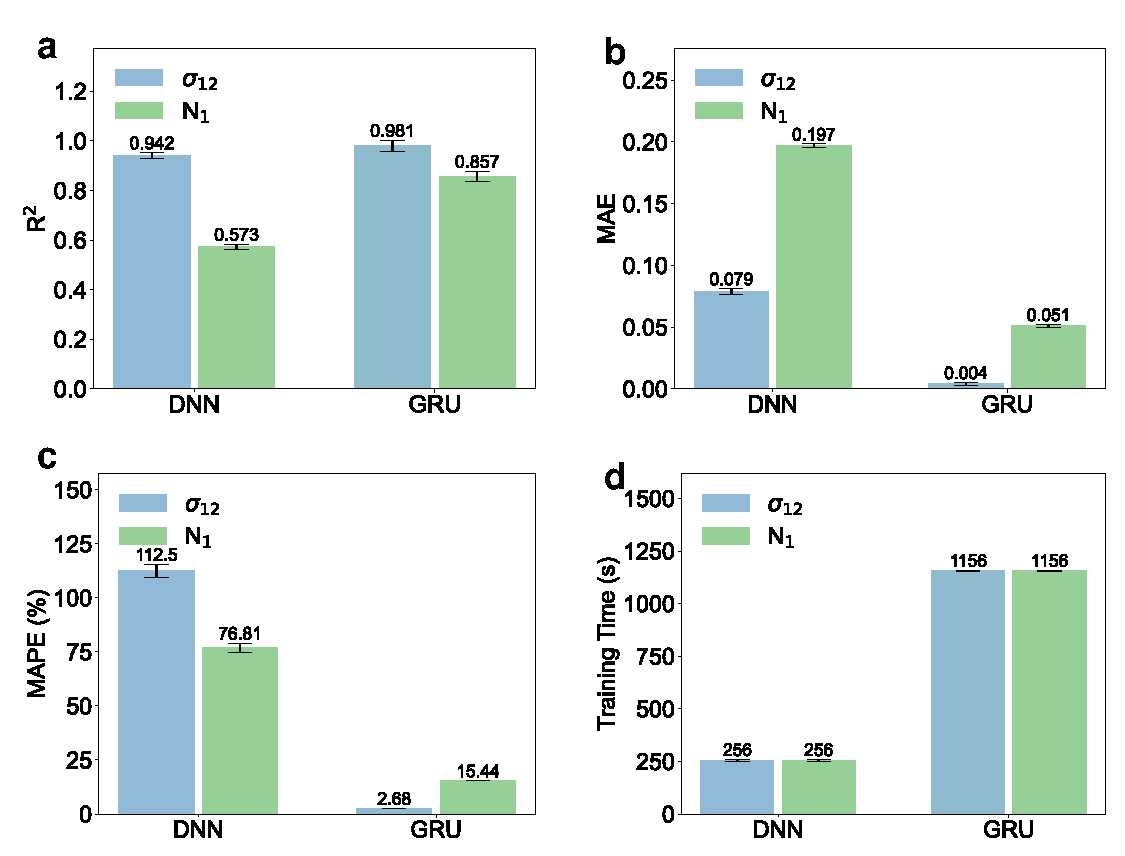
\includegraphics[width=0.8\textwidth]{Fig/giesekus-sin-metrics.pdf}
  \FigureBicaption{\label{giesekus-sin-metrics}GRU算法和DNN算法在Giesekus模型交变协议测试集上的预测效果对比示意图:(a)GRU和DNN在测试集上的R$^2$指标图;(b)GRU和DNN在测试集上的MAE指标图;(c)GRU和DNN在测试集上的MAPE指标图;(d)GRU和DNN在测试集上的训练时间指标图}{Comparison schematic of the prediction performance of the GRU algorithm and the DNN algorithm on the Giesekus model oscillatory protocol test set: (a) R$^2$ metric plots on the test set for GRU and DNN; (b) MAE metric plots on the test set for GRU and DNN; (c) MAPE metric plots on the test set for GRU and DNN; (d) Training Time metric plots on the test set for GRU and DNN}
\end{figure}
根据综合分析结果,当训练数据和测试数据均为交变应变时,GRU算法相比DNN能够更好地学习到Giesekus模型数据的内在特征。本节中,我们使用了SAOS和LAOS结合的训练数据,以探究模型对非线性黏弹性的学习能力。结果显示,GRU算法很好地完成了任务,成功捕捉了Giesekus模型模拟数据中的复杂非线性关系。综合来看,GRU算法在处理Giesekus模型的非线性黏弹性数据时表现出了显著的优越性,为后续研究提供了新的视角。

% Giesekus模型交变预测线性协议效果验证
\subsubsection{交变协议预测线性协议效果验证}
\begin{figure}[htbp]
  \centering
  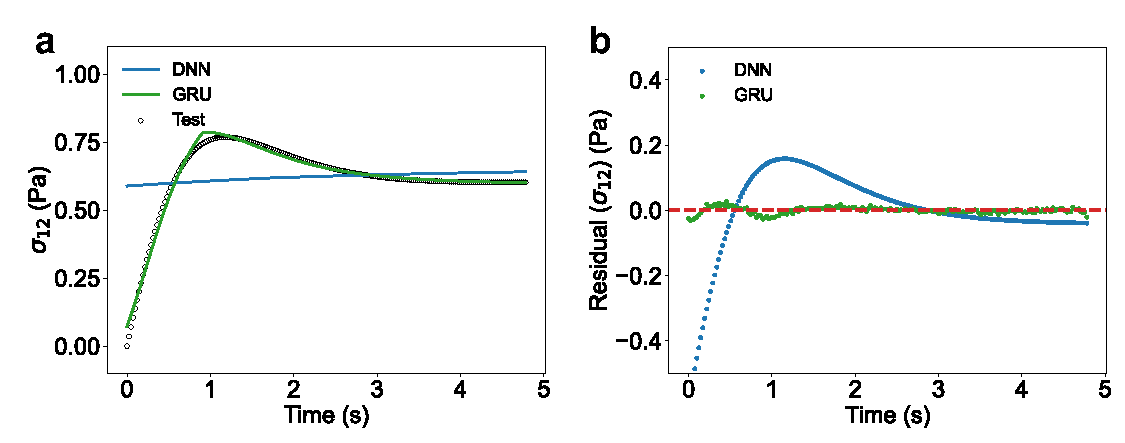
\includegraphics[width=0.8\textwidth]{Fig/giesekus-linear.pdf}
  \FigureBicaption{\label{giesekus-linear}GRU算法和DNN算法在Giesekus模型交变协议预测线性协议测试集上的预测效果对比示意图:(a)GRU和DNN在测试集上的时间-应力曲线;(b)GRU和DNN在测试集上的残差图}{Comparison schematic of the prediction performance of the GRU algorithm and the DNN algorithm on the Giesekus model oscillatory protocol predicting linear protocol test set: (a) Time-stress curves for GRU and DNN on test set; (b) Residual plots for GRU and DNN on test set}
\end{figure}
\begin{figure}[htbp]
  \centering
  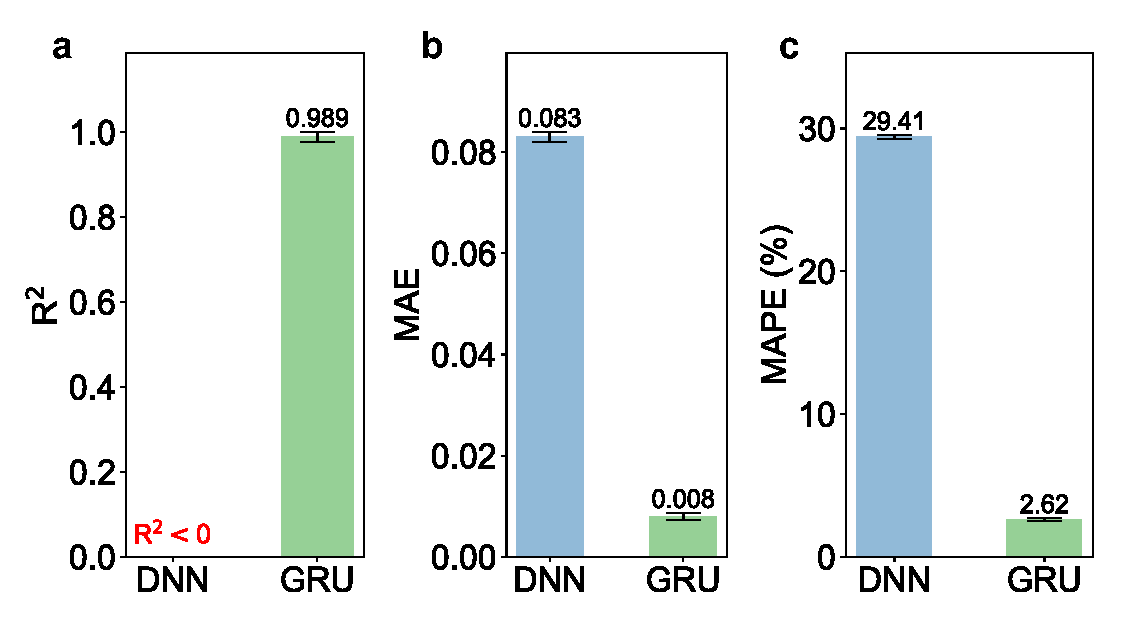
\includegraphics[width=0.8\textwidth]{Fig/giesekus-linear-metrics.pdf}
  \FigureBicaption{\label{giesekus-linear-metrics}GRU算法和DNN算法在Giesekus模型交变协议预测线性协议测试集上的预测效果对比示意图:(a)GRU和DNN在测试集上的R$^2$指标图;(b)GRU和DNN在测试集上的MAE指标图;(c)GRU和DNN在测试集上的MAPE指标图}{Comparison schematic of the prediction performance of the GRU algorithm and the DNN algorithm on the Giesekus model oscillatory protocol predicting linear protocol test set: (a) R$^2$ metric plots on the test set for GRU and DNN; (b) MAE metric plots on the test set for GRU and DNN; (c) MAPE metric plots on the test set for GRU and DNN}
\end{figure}
为了检验GRU算法在不同形式的应变历史下对Giesekus模型的泛化预测能力,本节采用交变应变协议生成的数据作为训练集,线性应变协议生成的数据作为测试集。分别使用GRU和DNN进行模型训练,并在测试集上进行验证,验证结果如图 \ref{giesekus-linear} 和图 \ref{giesekus-linear-metrics} 所示。

图\ref{giesekus-linear}(a)为两种不同算法预测模型在测试集上的真实值-预测值曲线,图中可以看到GRU算法的预测值的曲线与真实值曲线接近,仅在1-2 s之间存在小部分突出偏差,而DNN算法的预测值曲线完全没有拟合到曲线特征。图\ref{giesekus-linear}(b)展示了两种算法在测试集上的残差图。从图中可以明显看出,DNN算法的预测值与真实值之间的残差整体呈现出较为清晰的曲线趋势,存在明显的峰值。图中结果表明DNN完全没有捕捉到训练数据中的关键特征,导致其在测试集上的表现很差。与之形成鲜明对比的是,GRU 算法的残差图呈现出无序分布的特征,残差点均匀地分布贴近在 0 刻度线两侧。这一现象表明,GRU 能够更有效地学习数据中的关键特征,从而实现更小的预测偏差。结合真实值与预测值的曲线分析以及残差图的观察,可以分析出GRU在此项任务的预测性能优于DNN。


具体如图\ref{giesekus-linear-metrics} 所示。从图\ref{giesekus-linear-metrics}(a)可以清晰地观察到,GRU 算法的 R$^2$值高达 0.989,这一结果有力地表明了 GRU 在预测任务中的出色表现。与之形成鲜明对比的是,DNN算法的R$^2$值小于 0,这表明 DNN 并未有效学习到相关特征。进一步分析图\ref{giesekus-linear-metrics}(b-c),可以发现 GRU 预测结果的平均绝对误差(MAE)值为 0.008,而 DNN的 MAE 值则高达 0.083。这表明GRU 在绝对误差方面的表现仅为DNN的十分之一,优势极为明显。此外,GRU 预测结果的平均绝对百分比误差(MAPE)值为2.62\%,而DNN 的 MAPE 值则为 29.41\%。这些定量数据充分证明了 GRU 的预测结果误差小于 DNN,从而进一步证实了 GRU 在该任务上的预测泛化能力更强。
在两种算法的训练时间对比方面,与上一节中交变协议预测交变协议的情况相同,具体可参考图 \ref{giesekus-sin-metrics}(d)所示。

\subsubsection{不同时间步的预测效果对比}
\begin{figure}[htbp]
  \centering
  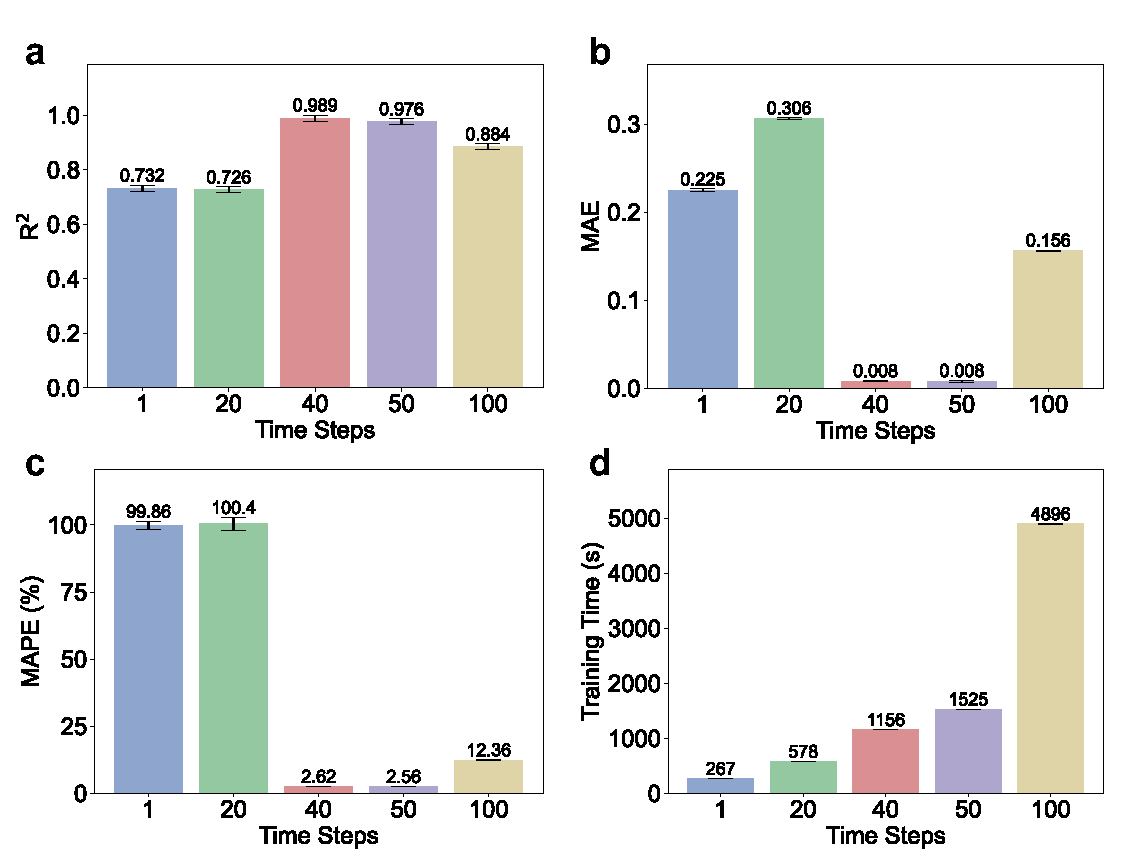
\includegraphics[width=0.8\textwidth]{Fig/giesekus-timesteps-metrics.pdf}
  \FigureBicaption{\label{giesekus-timesteps-metrics}GRU算法和DNN算法在Giesekus模型不同时间步长下的预测指标对比图:(a)GRU和DNN在不同时间步下的R$^2$指标图;(b)GRU和DNN在不同时间步下的MAE指标图;(c)GRU和DNN在不同时间步下的MAPE指标图;(d)GRU和DNN在不同时间步下的训练时间指标图}{Comparison schematic of the prediction performance of the GRU algorithm and the DNN algorithm under different time steps of the Giesekus model: (a) R$^2$ metric plots under different time steps for GRU and DNN; (b) MAE metric plots under different time steps for GRU and DNN; (c) MAPE metric plots under different time steps for GRU and DNN; (d) Training Time metric plots under different time steps for GRU and DNN}
\end{figure}
为了探究在Giesekus模型上GRU算法的最佳时间步,本节研究了不同时间步下训练的模型在测试集上的预测效果,如图\ref{giesekus-timesteps-metrics}所示。由图可见,预测模型R$^2$值在时间步小于40时为0.7左右,当时间步为40时为0.969,时间步进一步增加,R$^2$开始下降。MAE值在时间步为40相比20时从0.306调跃减少至0.008,进一步增加时间步,MAE值不再显著改变,直到时间步为100,MAE值回升至0.156,显现过拟合趋势。MAPE值变化趋势与MAE值类似,在时间步为40左右跳跃减少,随后直到100步开始回升。从训练时间来看,随着时间步增加,训练时间单调增加,这一点与预期一致。




\subsection{真实数据集实验}
为了验证我们的PI-GRU模型在真实数据集上的表现,本文选取了ABE弹性体数据集,训练数据集为SAOS和LAOS的混合数据集,测试集分为SAOS和LAOS数据两类以验证模型在线性区间和非线性区间的预测效果。由图\ref{fgr:real-data-differstrain}可知,PI-GRU模型在SAOS测试集上相比对比的XGBoost模型、多层感知器(MLP)模型、PI-MLP模型(该模型构建参考Mahmoudabadbozchelou)\cite{mahmoudabadbozchelouDatadrivenPhysicsinformedConstitutive2021}具有最佳的预测效果,预测指标(图\ref{fgr:real-data-differstrain-saos-metrics})中MAPE值仅为3.33\%,属于优秀泛化范畴,相比PI-MLP模型的14.9\%下降了11.57\%,在训练时间成本上,PI-GRU模型为1070s相比PI-MLP模型(789s)仅增加了281s。
\begin{figure}
  \centering
  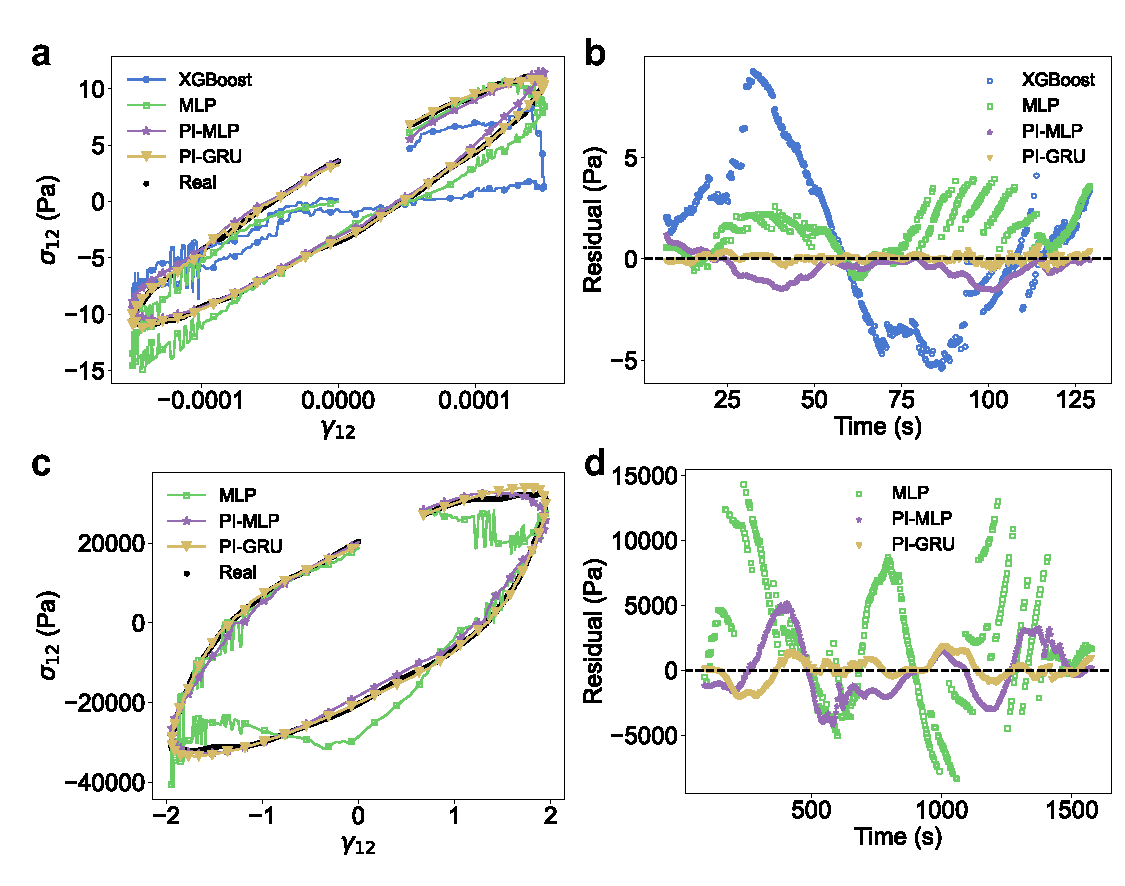
\includegraphics[width=0.8\textwidth]{Fig/real-data-differstrain.pdf} % 此处填写图片名
  \FigureBicaption{\label{fgr:real-data-differstrain}ABE弹性体的Lissajous曲线在不同算法上的预测效果:(a)小振幅振荡剪切(SAOS)测试集真实值与模型预测值的Lissajous曲线对比;(b)小振幅振荡剪切(SAOS)测试集真实值与模型预测值的残差图;(c)大振幅振荡剪切(LAOS)测试集真实值与模型预测值的Lissajous曲线对比;(d)大振幅振荡剪切(LAOS)测试集真实值与模型预测值的残差图}{Prediction performance comparison of Lissajous curves for ABE elastomer using different algorithms: (a) Comparison of Lissajous curves between true values and model predictions on small-amplitude oscillatory shear (SAOS) test set; (b) Residual plot of true values and model predictions on SAOS test set; (c) Comparison of Lissajous curves between true values and model predictions on large-amplitude oscillatory shear (LAOS) test set; (d) Residual plot of true values and model predictions on LAOS test set}
\end{figure}
\begin{figure}
  \centering
  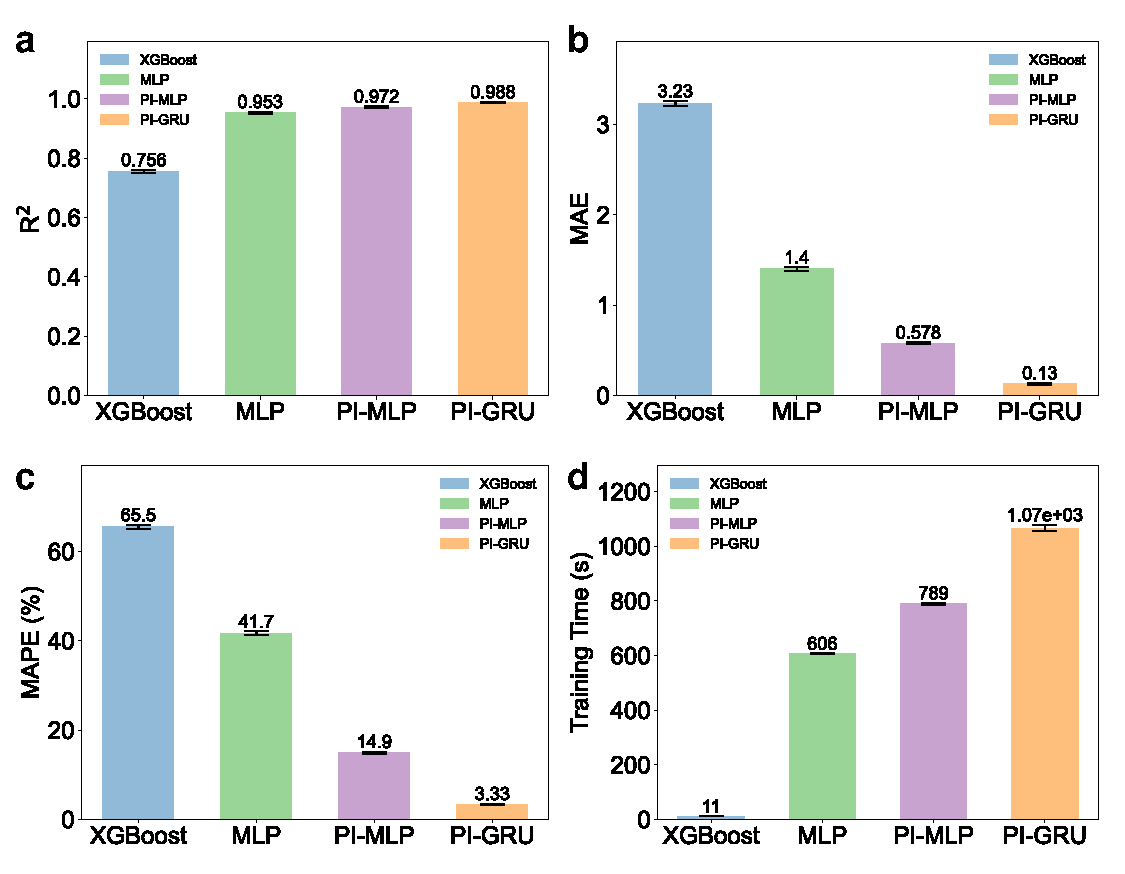
\includegraphics[width=0.8\textwidth]{Fig/real-data-differstrain-saos-metrics.pdf} % 此处填写图片名
  \FigureBicaption{\label{fgr:real-data-differstrain-saos-metrics}}{不同算法在ABE弹性体SAOS实验Lissajous曲线上的预测指标对比:(a)决定系数(R²),(b)平均绝对误差(MAE),(c)平均绝对百分比误差(MAPE),(d)计算训练时间}{Comparative Evaluation of Predictive Metrics for ABE Elastomer's Lissajous Curves in SAOS Experiments Across Algorithms: (a) Coefficient of Determination (R²), (b) Mean Absolute Error (MAE), (c) Mean Absolute Percentage Error (MAPE), (d) Computational Training Time}
\end{figure}

\begin{figure}
  \centering
  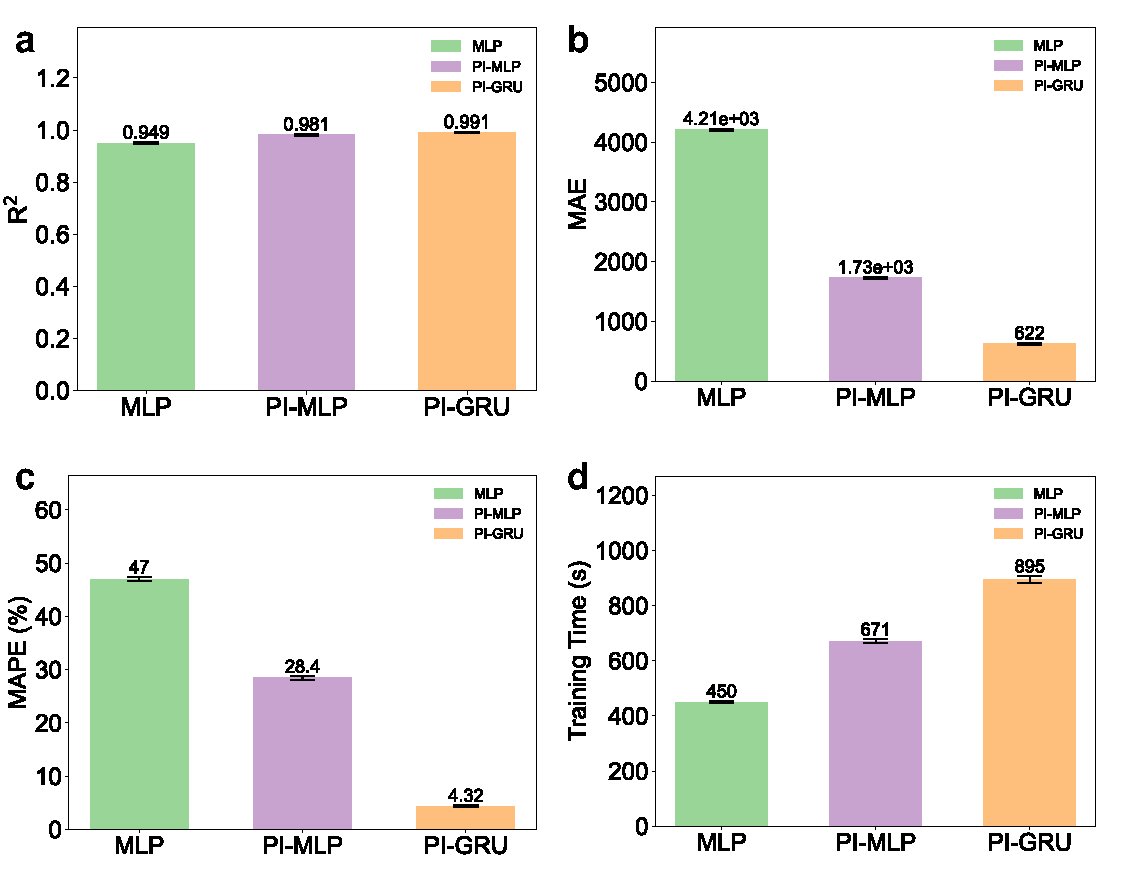
\includegraphics[width=0.8\textwidth]{Fig/real-data-differstrain-laos-metrics.pdf} % 此处填写图片名
  \FigureBicaption{\label{fgr:real-data-differstrain-laos-metrics}}{不同算法在ABE弹性体LAOS实验Lissajous曲线上的预测指标对比:(a)决定系数(R²),(b)平均绝对误差(MAE),(c)平均绝对百分比误差(MAPE),(d)计算训练时间}{Comparative Evaluation of Predictive Metrics for ABE Elastomer's Lissajous Curves in LAOS Experiments Across Algorithms: (a) Coefficient of Determination (R²), (b) Mean Absolute Error (MAE), (c) Mean Absolute Percentage Error (MAPE), (d) Computational Training Time}
\end{figure}
LAOS测试集上,如图\ref{fgr:real-data-differstrain}(c-d)所示,PI-GRU的表现大幅度领先对比模型,PI-GRU模型预测指标(图\ref{fgr:real-data-differstrain-laos-metrics})中MAPE值仅为4.32\%,相比PI-MLP模型的28.4\%下降了24.08\%,在训练时间成本上,PI-GRU模型为895s相比PI-MLP模型(671s)仅增加了224s。这一结果说明,PI-GRU模型在处理非线性黏弹性材料的流变学数据时,能够更好地捕捉到数据中的时间依赖性特征,这是因为门控单元可以自主决定是否记忆和遗忘信息,即对于每一个时间步的应变状态历史,门控单元自主给予不同的权重,从而更好地拟合非线性区应力历史叠加并非玻尔兹曼叠加原理的流变学数据,这一特性使得GRU结构相当于对黏弹性材料的历史依赖性做了特有的特征融合,这是作为前馈神经网络的MLP模型无法做到的。值得注意的是,在预测过程中,物理约束损失的本构方程形式为最简单的Maxwell模型(并未引入非线性点),然后就结果来看,PI-GRU模型依旧可以很好地泛化到非线性区间的LAOS数据,这是因为物理约束给予的是大致的物理规律符合,例如Oldroyd-B类模型(Giesekus、FENE-P、​LPTT)通过不同形式的非线性修正扩展了基础模型的适用范围,而GRU模型在Maxwell模型的物理约束下从另一种独特的形式修正扩展了基础模型。由于简单Maxwell模型的参数拟合非常简单,且本文的研究并不需要过分追求物理约束部分的本构方程的参数精确度,因此该模型可以低成本地扩展到其他不同的流变学实验体系。



% 本章小结 
\section{本章小结}

本章首先运用了门控循环单元(GRU)算法对数值模拟的 Herschel-Bulkley 模型、Maxwell 模型、Doi-Edwards 模型以及 Giesekus 模型所产生的模拟数据展开深度学习建模工作。

研究结果揭示出,GRU 作为一种循环神经网络,依托其独特的门控单元机制,能够精准地捕捉黏弹性材料流变学模拟数据所蕴含的时间依赖性以及复杂非线性特征。特别的,在处理 Herschel-Bulkley 模型这类非时间序列数据时,GRU 模型的预测效果相较于DNN(深度神经网络)模型依旧略胜一筹。究其原因,在于 GRU 的门控单元机制引入了更多的参数,从而赋予了其更佳的泛化性能。对于经典的简单 Maxwell模型,由于属于典型的时间序列数据,GRU对其进行建模预测的效果全面超越DNN,各项评估指标均展现出显著优势。当面对更为复杂Doi-Edwards 模型时,GRU的建模预测效果依旧优于 DNN。进一步分析发现,在相同的建模任务中,GRU 在剪切应力$\sigma_{12}$的预测效果上强于第一法向应力差N$_1$。在Giesekus 模型的研究中,本章模拟了小振幅振荡剪切(SAOS)以及大振幅振荡剪切(LAOS)这两种不同的工况。实验结果表明,GRU 的建模效果优于 DNN,这有力地说明 GRU 所捕捉的时间依赖性,不仅仅局限于基于玻尔兹曼叠加原理的线性黏弹性的时间特性,还能够涵盖更为复杂的非线性关系,而Giesekus模型下GRU对第一法向应力差N$_1$的预测效果也比$\sigma_{12}$差。

在本章模拟数据预测部分设计的实验中,我们探讨了两类预测任务:首先,利用交变应变变化的训练数据,预测相应的测试数据;其次,使用交变应变变化实验的训练数据,预测线性应变变化的测试数据。在针对不同本构模型的这两类实验中,GRU(门控循环单元)模型的表现均优于DNN(深度神经网络)。这一现象充分表明,GRU具备更强的泛化能力,能够有效地预测更为一般化的本构关系,而不仅仅是进行简单的函数逼近。GRU通过引入门控机制,能够有效捕捉序列数据中的长期依赖关系,从而在处理复杂的本构模型时展现出更优的性能。相比之下,DNN虽然在非时序本构模型中表现出色,但在处理具有复杂时序特征的本构模型时,其性能会受到限制。因此,选择GRU模型进行本构关系的预测,能够更好地适应数据的复杂性和多样性,提升预测的准确性和可靠性,但是本章的实验结果同样表明,GRU模型由于其架构特征,比普通DNN的训练时间高很多,且训练时消耗更多的计算机资源(计算机内存、GPU显存等)。

为了进一步探究GRU在真实数据集上的表现,本章选取了ABE弹性体的流变学实验数据集进行验证。使用简答Maxwell模型作为物理约束残差方程,设计物理信息约束的门控循环单元(PI-GRU)。通过将PI-GRU模型与XGBoost、MLP以及PI-MLP等模型进行对比,结果显示PI-GRU模型在测试集上表现最佳。特别值得注意的是,即使在物理约束采用最简单的Maxwell模型的情况下,PI-GRU模型仍然能够很好地泛化到非线性区间的LAOS数据,这充分证明了该模型在处理复杂流变学数据时的优越性。

综上所述,本章的研究工作充分验证了GRU在流变学数据建模中的优异效果。该模型不仅能够准确捕捉黏弹性材料的时间依赖性,从而高效刻画非线性、时变的物理过程,展现出良好的关联适配性,而且在理论上突破了传统数据拟合方法的局限,在模拟数据和真实实验数据中均表现出卓越的泛化能力和预测稳定性。总的来说,本章的研究为深度学习在流变学本构建模领域的应用开辟了全新的思路,即可以从模型升级的角度去优化本构建模的过程。





%第三章
\chapter{列举环境}
以下资料来自宏包说明和网络,翻译不一定正确:

在LaTeX中有三种基本的列举(列表)环境,即enumerate(编号)、itemize(分条目)和description(描述)环境。调整latex的列表环境时,使用 enumitem 宏包可以方便的调整间距(注意区分包名和环境名)和自定义编号样式。

\section{调整间距}
三种基本环境无论哪一种,间距的调整都是一样的。调整间距的参数命令包括两类:垂直间距和水平间距。各种距离的定义如图\ref{enumitem}所示。下图的来源一直找不到,可能是旧版本的宏包说明,新版已经删掉了下面的注释了。
\begin{figure}[htbp]
	\centering
	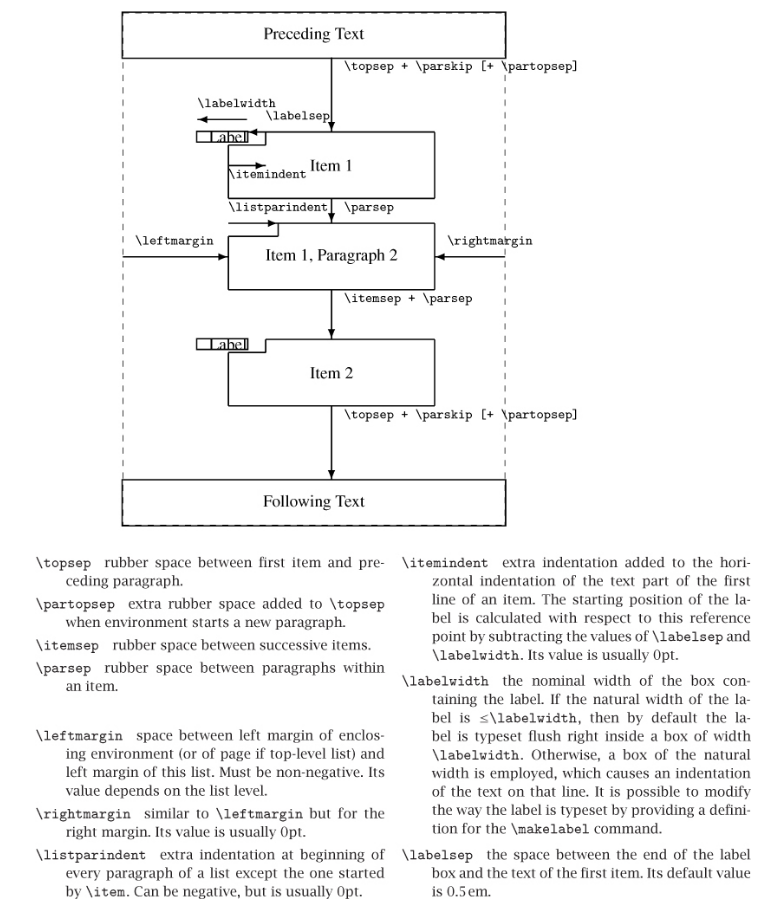
\includegraphics[scale=0.6]{Fig/enumitem1.png}
	\caption{\label{enumitem}enumitem包对各种间距的定义}
\end{figure}

现先总结出所推荐的间距设置,无编号的:
\begin{lstlisting}
\begin{itemize}[topsep = 0 pt, itemsep= 0 pt, parsep=0pt, partopsep=0pt, leftmargin=36pt, itemindent=0pt, labelsep=6pt, listparindent=24pt]
	\item 第一项。内容内容内容内容内容内容内容内容内容内容内容内容内容内容内容内容内容内容内容内容内容内容内容内容内容内容内容内容内容内容

	\item 第二项。内容内容内容内容内容内容内容内容内容内容内容内容内容内容内容内容内容内容内容内容内容内容内容内容内容内容内容内容内容内容
	
\end{itemize}
\end{lstlisting}
效果:
\begin{itemize}[topsep = 0 pt, itemsep= 0 pt, parsep=0pt, partopsep=0pt, leftmargin=36pt, itemindent=0pt, labelsep=6pt, listparindent=24pt]
	\item 第一项。内容内容内容内容内容内容内容内容内容内容内容内容内容内容内容内容内容内容内容内容内容内容内容内容内容内容内容内容内容内容

	\item 第二项。内容内容内容内容内容内容内容内容内容内容内容内容内容内容内容内容内容内容内容内容内容内容内容内容内容内容内容内容内容内容
	
\end{itemize}

有编号的:
\begin{lstlisting}
\begin{enumerate}[topsep = 0 pt, itemsep= 0 pt, parsep=0pt, partopsep=0pt, leftmargin=44pt, itemindent=0pt, labelsep=6pt, label=(\arabic*)]
	\item 第一项。内容内容内容内容内容内容内容内容内容内容内容内容内容内容内容内容内容内容内容内容内容内容内容内容内容内容内容内容内容内容

	\item 第二项。内容内容内容内容内容内容内容内容内容内容内容内容内容内容内容内容内容内容内容内容内容内容内容内容内容内容内容内容内容内容
	
\end{enumerate}
\end{lstlisting}
效果:
\begin{enumerate}[topsep = 0 pt, itemsep= 0 pt, parsep=0pt, partopsep=0pt, leftmargin=44pt, itemindent=0pt, labelsep=6pt, label=(\arabic*)]
	\item 第一项。内容内容内容内容内容内容内容内容内容内容内容内容内容内容内容内容内容内容内容内容内容内容内容内容内容内容内容内容内容内容

	\item 第二项。内容内容内容内容内容内容内容内容内容内容内容内容内容内容内容内容内容内容内容内容内容内容内容内容内容内容内容内容内容内容
	
\end{enumerate}

下面两节分别讨论参数设置规则。
\subsection{垂直间距}
摘抄宏包说明:
\begin{itemize}[topsep = 0 pt, itemsep= 0 pt, parsep=0pt, partopsep=0pt, leftmargin=36pt, itemindent=0pt, labelsep=6pt, listparindent=24pt]
	\item topsep控制列表环境与上文之间的距离。第一项和前一段之间的空间。

	\item itemsep 条目之间的距离

	\item parsep 条目里面段落之间的距离
 
	\item partopsep 条目与下面段落的距离。当环境开始一个新段落时,额外的空间被添加到 \textbackslash{}topsep。
\end{itemize}

论文中希望上述距离都为0pt,如:
\begin{lstlisting}
	\begin{itemize}[topsep = 0 pt, itemsep= 0 pt, parsep=0pt, partopsep=0pt]
		\item 第一项。
		\item 第二项
		\item 第三项。
	\end{itemize}
\end{lstlisting}
效果为:
\begin{itemize}[topsep = 0 pt, itemsep= 0 pt, parsep=0pt, partopsep=0pt]
	\item 第一项。
	\item 第二项
	\item 第三项。
\end{itemize}


\subsection{水平间距}
% 正文12pt
水平间距调整比较复杂,对照宏包说明给出的图,下面内容参考了宏包原文和网络资料:
\begin{itemize}[topsep = 0 pt, itemsep= 0 pt, parsep=0pt, partopsep=0pt, leftmargin=36pt, itemindent=0pt, labelsep=6pt, listparindent=24pt]
	\item 为页面的左边距)和该列表的左边距之间的空间。 必须是非负数。 它的值取决于表,则为页面的左边距)和该列表的左边距之间的空间。 必须是非负数。 它的值取决于列表级别。
	\item rightmargin       列表环境右边的空白长度。类似于 \textbackslash{}leftmargin 但用于右边距。 它的值通常是 0pt。
	\item labelsep       标号与列表第一项文本左侧的距离。标签框的末尾和第一项的文本之间的空间。 它的默认值为 0.5 em。
	\item itemindent       条目的缩进距离。添加到项目第一行文本部分的水平缩进的额外缩进。 通过减去 labelsep 和 labelwidth 的值,相对于该参考点计算标签的起始位置。 它的值通常是 0pt。注:理解这个变量时,查看图\ref{enumitem}的顺序应该按照箭头从左到右,先leftmargin再itemindent,然后再labelsep,最后labelwidth。即箭头的起始点是基准点。若itemindent=0pt,则leftmargin-labelsep-编号长度的结果就是编号起始位置。
	\item labelwidth       包含标签的框的标称宽度。 如果标签的自然宽度为 < labelwidth,则默认情况下,标签在宽度为 (labelwidth) 的框内右对齐排版。否则,使用自然宽度的框,这会导致该行上的文本缩进。 可以通过为 \textbackslash{}makelabel 命令提供定义来修改标签的排版方式。
	\item listparindent       条目下面段落的缩进距离。除了以 litem 开头的段落之外,列表的每个段落的开头都有额外的缩进。 可以为负数,但通常为 0pt。
\end{itemize}

无编号的水平间距,给出两张方案
 
第一种:
\begin{itemize}[topsep = 0 pt, itemsep= 0 pt, parsep=0pt, partopsep=0pt, leftmargin=36pt, itemindent=0pt, labelsep=6pt, listparindent=24pt]
	\item 第一项。内容内容内容内容内容内容内容内容内容内容内容内容内容内容内容内容内容内容内容内容内容内容内容内容内容内容内容内容内容内容

	% 第一项的第二段。内容内容内容内容内容内容内容内容内容内容内容内容内容内容内容内容内容内容内容内容内容内容内容内容内容内容内容内容内容内容
	\item 第二项。内容内容内容内容内容内容内容内容内容内容内容内容内容内容内容内容内容内容内容内容内容内容内容内容内容内容内容内容内容内容
	
\end{itemize}


第二种:
\begin{itemize}[topsep = 0 pt, itemsep= 0 pt, parsep=0pt, partopsep=0pt, leftmargin=0pt, itemindent=36pt, labelsep=6pt, listparindent=24pt]
	\item 第一项。内容内容内容内容内容内容内容内容内容内容内容内容内容内容内容内容内容内容内容内容内容内容内容内容内容内容内容内容内容内容

	% 第一项的第二段。内容内容内容内容内容内容内容内容内容内容内容内容内容内容内容内容内容内容内容内容内容内容内容内容内容内容内容内容内容内容
	\item 第二项。内容内容内容内容内容内容内容内容内容内容内容内容内容内容内容内容内容内容内容内容内容内容内容内容内容内容内容内容内容内容
	
\end{itemize}

推荐第一种。

有编号的水平间距,下面给出三种方案:
注:labelsep是某一项文字和编号框的距离,一般就设为一个空格6pt,要使编号左侧缩进两格,itemindent-labelsep要等于编号长度。注意编号是右对齐,向左扩展的。

第一种方案是整体右移两格,文字距离编号一个空格,然后第二行文字和第一行对齐:
\begin{enumerate}[topsep = 0 pt, itemsep= 0 pt, parsep=0pt, partopsep=0pt, leftmargin=44pt, itemindent=0pt, labelsep=6pt, label=(\arabic*)]
	\item 第一项。内容内容内容内容内容内容内容内容内容内容内容内容内容内容内容内容内容内容内容内容内容内容内容内容内容内容内容内容内容内容

	% 第一项的第二段。内容内容内容内容内容内容内容内容内容内容内容内容内容内容内容内容内容内容内容内容内容内容内容内容内容内容内容内容内容内容
	\item 第二项。内容内容内容内容内容内容内容内容内容内容内容内容内容内容内容内容内容内容内容内容内容内容内容内容内容内容内容内容内容内容
	
\end{enumerate}

第二种方案是和论文撰写规范的格式一样,注意不是论文撰写规范规定的格式,规范里没有规定这些格式。如:
\begin{enumerate}[topsep = 0 pt, itemsep= 0 pt, parsep=0pt, partopsep=0pt, leftmargin=0pt, itemindent=44pt, labelsep=6pt, listparindent=24pt, label=(\arabic*)]
	\item 第一项。内容内容内容内容内容内容内容内容内容内容内容内容内容内容内容内容内容内容内容内容内容内容内容内容内容内容内容内容内容内容

	% 第一项的第二段。内容内容内容内容内容内容内容内容内容内容内容内容内容内容内容内容内容内容内容内容内容内容内容内容内容内容内容内容内容内容
	\item 第二项。内容内容内容内容内容内容内容内容内容内容内容内容内容内容内容内容内容内容内容内容内容内容内容内容内容内容内容内容内容内容
	
\end{enumerate}

第三种方案是整体右移两格,文字距离编号一个空格,第二行文字不再右移:
\begin{enumerate}[topsep = 0 pt, itemsep= 0 pt, parsep=0pt, partopsep=0pt, leftmargin=24pt, itemindent=20pt, labelsep=6pt, listparindent=20pt, label=(\arabic*)]
	\item 第一项。内容内容内容内容内容内容内容内容内容内容内容内容内容内容内容内容内容内容内容内容内容内容内容内容内容内容内容内容内容内容

	% 第一项的第二段。内容内容内容内容内容内容内容内容内容内容内容内容内容内容内容内容内容内容内容内容内容内容内容内容内容内容内容内容内容内容
	\item 第二项。内容内容内容内容内容内容内容内容内容内容内容内容内容内容内容内容内容内容内容内容内容内容内容内容内容内容内容内容内容内容
	
\end{enumerate}

推荐第一种。

\section{enumerate标签样式}
除上述小括号数字的编号方法外,还有斜体字母等。在使用enumerate的时候,label的问题就是使用计数的字符,是阿拉伯数字、罗马、中文、还是希腊字符的问题。

\subsection{小括号阿拉伯数字}
% 小括号阿拉伯数字,用 label=\arabic*)
\begin{enumerate}[topsep = 0 pt, itemsep= 0 pt, parsep=0pt, partopsep=0pt, leftmargin=0pt, itemindent=44pt, labelsep=6pt, listparindent=24pt, label=\arabic*)]
	\item 第一项。

	% 第一项的第二段。
	\item 第二项
	
	% 第二项的第二段。
	\item 第三项。
	
	% 第三项的第二段。
\end{enumerate}



\subsection{斜体字母}
% 斜体字母,用 label=\emph{\alph*}
\begin{enumerate}[topsep = 0 pt, itemsep= 0 pt, parsep=0pt, partopsep=0pt, leftmargin=0pt, itemindent=44pt, labelsep=6pt, listparindent=24pt, label=\emph{\alph*}.]
	\item 第一项。

	% 第一项的第二段。
	\item 第二项
	
	% 第二项的第二段。
	\item 第三项。
	
	% 第三项的第二段。
\end{enumerate}

\subsection{大写罗马字母}
% 大写罗马字母,用 label=(\Roman*)
\begin{enumerate}[topsep = 0 pt, itemsep= 0 pt, parsep=0pt, partopsep=0pt, leftmargin=0pt, itemindent=44pt, labelsep=6pt, listparindent=24pt, label=(\Roman*)]
	\item 第一项。

	% 第一项的第二段。
	\item 第二项
	
	% 第二项的第二段。
	\item 第三项。
	
	% 第三项的第二段。
\end{enumerate}
%\chapter{公式字体选项——新增功能}
2024年陆续有同学提出公式数学符号字体不对,于是有了\url{https://github.com/mengchaoheng/SCUT_thesis/issues/81}的讨论——数学公式字体应该使用什么?这里简单提一下:

1)如果十分确定自己使用什么字体,或者对unicode-math的兼容性问题无法忍受,又或者持保守态度,不想冒险使用“新字体”,那不要改任何设置,使用默认的 Computer Modern 即可,因为模板的有效性已经由很多届同学验证,我反复提到这句话是因为,我们只是写毕业论文,不是成为latex专家,不要在修改模板上花时间,尽量使用现有的东西。不想折腾字体的同学可以不用继续往下看本章了。

2)若还是非常执著于修改公式字体,那可以试试所有OpenType math字体,XITS Math是我看比较合适的一种。在导言区或者cls文件加入
\begin{lstlisting}
\usepackage{unicode-math} 
\setmathfont{XITS Math}[math-style=ISO,bold-style=ISO] 
\setmathfont{XITS Math}[range={cal, bfcal}, StylisticSet=1] 
\end{lstlisting}
即实现了通过unicode-math宏包设置XITS Math字体并设置了选项[math-style=ISO,bold-style=ISO]。具体功能可以查看宏包文件。

本章摘选一些公式作为公式字体测试,同学们可以换成自己的文本,测试不同公式字体设置的效果。更多字体测试文件在math\_font文件夹。或者在\url{https://github.com/mengchaoheng/OpenType-MATH-TTF}对比多种字体效果。注意基本的符号规范,可在math\_font文件夹翻一翻基本内容。

\section{建模}
\label{sec:1}
\subsection{符号约定}
机体系的原点位于重心,正交的机体轴线表示为$\text{ }\!\!\{\!\!\text{ }{\boldsymbol{X}^{B}},{\boldsymbol{Y}^{B}},{\boldsymbol{Z}^{B}}\text{ }\!\!\}\!\!\text{ }$。 无人机沿机身轴线的角速度表示为${{\boldsymbol{\omega }}^{B}}=[p \quad q \quad r]^{T}$。风扇的转速记为$\Omega$。 每个控制舵的偏转角表示为 ${{\delta }_{i}}$,以矢量形式描述为$[{{\delta }_{1}} \quad {{\delta }_{2}} \quad {{\delta }_{3}} \quad {{\delta }_{4}}]^T$。



惯性系中的速度、惯性系中的姿态和风速分别表示为${{\boldsymbol{V}}^{I}}$,$\boldsymbol{\eta }$ 和 ${{\boldsymbol{W}}^{I}}$。 
由于涵道风扇无人机对所有机身轴对称,无人机的惯性矩阵可以简化为对角矩阵,表示为 $ \boldsymbol{I}=\text{diag}({{I}_{x} },{{I}_{y}},{{I}_{z}}) $。

在机体坐标系中表示的合力矩表示为 $\boldsymbol M$ ,为以下几项的和:
\begin{equation}
	{\boldsymbol{M}} = {{\boldsymbol{M}}_\text{vane}} + \boldsymbol{M}_{\text{flap}} + {\boldsymbol{M}}_{\text{fan}} + {\boldsymbol{M}}_{\text{aero}}
	\label{eq_1}
\end{equation}
其中 $ {{\boldsymbol{M}}_\text{vane}} $ 是从控制舵产生的控制力矩矢量。 $ \boldsymbol{M}_{\text{flap}} $ 是作用在固定气动襟翼上的反扭矩作用。 $ {\boldsymbol{M}}_{\text{fan}} $ 包括来自旋转的风扇的气动扭矩、角加速度力矩和陀螺效应。 $  {\boldsymbol{M}}_{\text{aero}} $ 是气动力矩。

\subsection{控制力矩}
四个控制舵的总控制力矩可以通过以下公式表示:
\begin{equation}
{{\boldsymbol{M}}_\text{vane}} = {k_{cv}}V_e^2\left[ {\begin{array}{*{20}{c}}
	{{\rm{ - }}{l_1}}&0&{{l_1}}&0\\
	0&{{\rm{ - }}{l_1}}&0&{{l_1}}\\
	{{l_2}}&{{l_2}}&{{l_2}}&{{l_2}}
	\end{array}} \right]{\boldsymbol{\delta }}
\label{eq_2}
\end{equation}
其中 $ {{k}_{cv}} $ 是与舵形状相关的常数系数。 $ {{l}_{1}} $ 和 $ {{l}_{2}} $ 是图中所示的杠杆臂。 ${{V}_{e}}$ 表示涵道流出的速度,由下式给出:
\begin{equation}
	{V_e} = {k_v}\Omega 
	\label{eq_3}
\end{equation}
其中 $ {{k}_{v}} $ 是与涵道的所有空气动力学特征相结合的常系数。 

如果所有舵偏转角都保持在气动失速极限内,则式 \eqref{eq_2} 中的比例关系成立,表示为 $ {{\delta }_{m}} $。 这是 ${\boldsymbol \delta}$ 的基本约束:
\begin{equation} 
	- {\delta _m} \le {\delta _i} \le {\delta _m},   i = 1,2,3,4.
	\label{eq_4}
\end{equation}

显然,式\eqref{eq_2} 将冗余舵偏转角映射到三维的控制力矩,表明无人机角速度子系统的过度驱动特性。 通过使用虚拟控制输入$ \boldsymbol{\nu }=[{\nu }_{x} \quad {\nu }_{y} \quad {\nu }_{z}]^{T}$,可以将控制力矩效应重构为模块化形式:
\begin{equation}
	\left\{ \begin{array}{l}
	{{\boldsymbol{I}}^{ - 1}}{{\boldsymbol{M}}_\text{vane}} = {{\boldsymbol{H}}_1}{\boldsymbol{\nu }}{\Omega ^2}\\
	{\boldsymbol{\nu }} = {\boldsymbol{B\delta }}
	\end{array} \right.
	\label{eq_5}
	\end{equation}
其中
	\begin{equation}
	\begin{array}{ccccc}
	{{\boldsymbol{H}}_1} \buildrel \Delta \over =   {k_{cv}}k_v^2\left[ {\begin{array}{*{20}{c}}
		{2I_x^{ - 1}{l_1}}&{}&{}\\
		{}&{2I_y^{ - 1}{l_1}}&{}\\
		{}&{}&{4I_z^{ - 1}{l_2}}
		\end{array}} \right]     \quad
	{\boldsymbol{B}} \buildrel \Delta \over =   \left[ {\begin{array}{*{20}{c}}
		{ - 0.5}&0&{0.5}&0\\
		0&{ - 0.5}&0&{0.5}\\
		{0.25}&{0.25}&{0.25}&{0.25}
		\end{array}} \right]
	\end{array}
	\label{eq_6}
\end{equation}

\section{控制器设计}


\subsection{控制分配}
对给定的 ${{\boldsymbol{\nu }}_{d}}$ 求解适当的舵偏转角 $\boldsymbol{\delta }$,
\begin{equation}
	{\boldsymbol {\nu}_d}={\boldsymbol{B\delta}}
	\label{eq_29.5}
\end{equation}
上式的解表示为 $\boldsymbol{\delta }_d$。 具体可以描述为:对于给定的${{\boldsymbol{\nu }}_{d}}$,求${{\boldsymbol{\delta }}_{d}}\in \Delta $使得 ${{\boldsymbol{\nu }}_{d}}=\boldsymbol{B}{{\boldsymbol{\delta }}_{d}}$,或者最小化分配误差 ${{\boldsymbol{\ nu }}_{d}}-\boldsymbol{B}{{\boldsymbol{\delta }}_{d}}$,其中 $\Delta $ 是允许控制集,定义为:
\begin{equation}
	\Delta=\left\{\boldsymbol{\delta} \in \mathbb{R}^{4} \mid-\delta_{m} \leq \delta_{i} \leq \delta_{m}, i=1,2,3,4\right\}
	\label{eq_30}
\end{equation}
如果 ${{\boldsymbol{\nu }}_{d}}$ 包含在可达集 (AS) 中,则称它是可达到的,可达集记为 $A$ 并定义为:
\begin{equation}
	A=\left\{\boldsymbol{\nu} \in \mathbb{R}^{3} \mid \boldsymbol{\nu}=\boldsymbol{B} \boldsymbol{\delta}, \boldsymbol{\delta} \in \Delta\right\}
	\label{eq_31}
\end{equation}

为了达到控制分配的目的,一种广泛采用的方法是直接计算 $\ç{B}$ 的伪逆:
\begin{equation}
	{{\boldsymbol{\delta }}_d} = {{\boldsymbol{B}}^\dag }{{\boldsymbol{\nu }}_d},   \quad  {{\boldsymbol{B}}^\dag } = {{\boldsymbol{B}}^T}{\left( {{\boldsymbol{B}}{{\boldsymbol{B}}^T}} \right)^{ - 1}}
	\label{eq_32}
\end{equation}

PCA 算法通过解决以下优化问题:
\begin{equation}
	\begin{aligned}
	&\max _{\alpha, \boldsymbol{\delta}} \alpha\\
	&\text { s.t. }\left\{\begin{array}{l}
	\boldsymbol{\delta} \in \Delta \\
	\boldsymbol{B} \boldsymbol{\delta}=\boldsymbol{\tau}_{i}+\alpha \boldsymbol{\tau}_{f} \\
	0 \leq \alpha \leq 1
	\end{array}\right.
	\end{aligned}
	\label{eq_pca}
\end{equation}
其中 $ \boldsymbol{B} $、$ \Delta $ 分别由式 \eqref{eq_6}、\eqref{eq_30} 定义。 $ \boldsymbol{\tau}_{i} $ 和 $ \boldsymbol{\tau}_{f} $ 在式 \eqref{eq_28} 中定义。



\section{控制理论}

\subsection{坐标变换}
考虑一个多输入多输出的非线性系统,其形式描述为
\begin{equation}
  \begin{aligned}
    \dot{\boldsymbol{x}}&=\boldsymbol{f}(\boldsymbol{x})+\boldsymbol{G}(\boldsymbol{x})\boldsymbol{u} + \boldsymbol{d}(x)\\
    \boldsymbol{y}&=\boldsymbol{h}(\boldsymbol{x})
  \end{aligned}
  \label{system}
\end{equation}

其中,$\boldsymbol{f}: \mathbb{R}^{n}\to\mathbb{R}^{n}$ 和 $\boldsymbol{h}: \mathbb{R}^{n}\to\mathbb{R}^{p}$ 是光滑的向量场。$\boldsymbol{G}$ 是一个光滑函数,将 $\mathbb{R}^{n}\to\mathbb{R}^{n\times m}$ 映射,其中的列是光滑的向量场。$\boldsymbol{d}: \mathbb{R}^{n}\to\mathbb{R}^{n}$ 是外部扰动向量。$\boldsymbol{y}\in\mathbb{R}^{P}$ 是被控制的输出向量,可以是系统可观测输出的任意子集的函数

设 $h$ 的元素为 $h_i, i = 1, 2, ..., p$,矩阵 $G$ 的列向量为 $g_j, j = 1, 2, ..., m$,则 $h_i$ 对向量场 $f$ 和 $g_j$ 的 Lie 导数定义为
\begin{equation}
  \mathcal{L}_{f}h_{i}=\frac{\partial h_{i}}{\partial x}f,\quad\mathcal{L}_{g_{j}}h_{i}=\frac{\partial h_{i}}{\partial x}g_{j},\quad\mathcal{L}_{f}^{k}h_{i}=\frac{\partial(\mathcal{L}_{f}^{k-1}h_{i})}{\partial x}f,\quad\mathcal{L}_{g_{j}}\mathcal{L}_{f}^{k}h_{i}=\frac{\partial(\mathcal{L}_{f}^{k}h_{i})}{\partial x}g_{j}
\end{equation}

以下两项假设是所有讨论的前提:

\begin{assumption}\label{assumption1}
  系统形式为

\end{assumption}
 
\begin{assumption}\label{assumption2}
  对于每个 
\end{assumption}

\begin{remark}
  矩阵
\end{remark}

\begin{remark}
  假设 2 是为了
\end{remark}

在假设 \ref{assumption1} 下

\begin{equation}
	\left.\left[\begin{array}{c}y_1^{(\gamma_1)}\\y_2^{(\gamma_2)}\\\vdots\\y_p^{(\gamma_p)}\end{array}\right.\right]=\left[\begin{array}{cccc}\mathcal{L}_f^{\gamma_1}h_1(x)\\\\\mathcal{L}_f^{\gamma_2}h_2(x)\\\vdots\\\mathcal{L}_f^{\gamma_p}h_p(x)\end{array}\right] +  \beta(x)  \boldsymbol{u}
  \end{equation}
  或者
  \begin{equation}
	y^{(\gamma)}=\alpha(x) + \beta(x) \boldsymbol{u}
	\label{outputdynamic}
  \end{equation}
  并且行向量 $dh_{1}(x),\ldots,dL_{f}^{\gamma_{1}-1}h_{1}(x),\ldots,dh_{p}(x),\ldots,dL_{f}^{\gamma_{p}-1}h_{p}(x)$ 是线性无关的。那么系统的相对度 $\gamma$ 满足 $\gamma=\|\gamma\|_{1}=\sum_{i=1}^{p}\gamma_{i}\leq n$,并且 $h_i(x),L_{f}h_i(x),\ldots,L_{f}^{\gamma_{i}-1}h_i(x)$,$1\leq i\leq p$ 可以作为新坐标的一部分。对于 $1\leq i\leq p$,设 
  \begin{equation}
	\begin{aligned}
	  \phi_{1}^{i}(x)&= h_{i}(x)\\
	  \phi_{2}^{i}(x)&= L_{f}h_{i}(x)\\
	  &\vdots\\
	  \phi_{\gamma_{i}}^{i}(x)&= L_{f}^{\gamma_{i}-1}h_{i}(x) 
	\end{aligned}
  \end{equation}
  如果 $\gamma  = n$,对于每个 $\boldsymbol{x} \in  \mathbb{D}$,存在一个邻域 $\mathbb{N}$,使得映射 
  \begin{equation}
  \Phi=[\phi_{1}^{1}(x),\ldots,\phi_{\gamma_1}^{1}(x),\ldots,\phi_{1}^{p}(x),\ldots,\phi_{\gamma_{p}}^{p}(x)]^{T}
  \end{equation}
  在 $\mathbb{N}$ 上是一个微分同胚。否则,如果 $\gamma < n$,对于每个 $\boldsymbol{x} \in  \mathbb{D}$,总可以找到光滑函数 $\phi_{r+1}(x),\ldots,\phi_{n}(x)$,使得
  \begin{equation}
	\Phi=[\phi_{1}^{1}(x),\ldots,\phi_{\gamma_1}^{1}(x),\ldots,\phi_{1}^{p}(x),\ldots,\phi_{\gamma_{p}}^{p}(x),\phi_{\gamma+1}(x),\ldots,\phi_{n}(x)]^{T}
  \end{equation}
  在 $\boldsymbol{x}$ 的邻域 $\mathbb{N}$ 上是一个微分同胚。根据假设 \ref{assumption2},根据 Frobenius 定理,总是可以选择 $\phi_{r+1}(x),\ldots,\phi_{n}(x)$,使得对所有 $r+1\leq i\leq n$ 和所有 $1\leq j\leq m$,有 $L_{g_{j}}\phi_{i}(x)=0$,对于所有 $x \in \mathbb{N}$。 
  
  总之,如果假设 \ref{assumption1} 和 \ref{assumption2}(对于 $\gamma < n$)成立,并且忽略外部干扰,总可以找到适当的局部坐标变换 $\phi(x)$,在其下,原始系统 \eqref{system} 可以表示为标准形式。设 
  \begin{equation}
	\xi^i=\begin{pmatrix}\xi_1^i\\\xi_2^i\\\vdots\\\xi_{\gamma_i}^i\end{pmatrix}=\begin{pmatrix}\phi_1^i(x)\\\phi_2^i(x)\\\vdots\\\phi_{\gamma_i}^i(x)\end{pmatrix} \quad  
	  \xi=\begin{pmatrix}\xi^1 \\ \vdots \\ \xi^m\end{pmatrix} \quad  
	  \eta=\begin{pmatrix}\eta_1\\\eta_2\\\vdots\\\eta_{n-\gamma}\end{pmatrix}=\begin{pmatrix}\phi_{\gamma+1}(x)\\\phi_{\gamma+2}(x)\\\vdots\\\phi_n(x)\end{pmatrix} \quad   
	  z=\Phi(x)=\begin{pmatrix}\xi\\\eta\end{pmatrix}
	  \label{stran}
  \end{equation}
  然后,方程 \eqref{system} 可以重写为标准形式,为简便起见,我们仍然保留原始坐标,并以向量形式重写系统 \eqref{system} 的标准形式:
  \begin{equation}
	\begin{aligned}&\dot{\eta}= f_{0}(\eta,\xi)\\&\dot{\xi}= A_{c}\xi+B_{c}[\alpha(x)+\beta(x)u]\\&\text{y}= C_{c}\xi\end{aligned}
  \end{equation}
  % \section{增量非线性动态逆的重表述}
  其中 
  \begin{equation}
	A_c=\mathrm{diag}(A_{1},\ldots,A_{m})\quad B_c=\mathrm{diag}(B_{1},\ldots,B_{m})\quad C_c=\mathrm{diag}(C_{1},\ldots,C_{m})
  \end{equation}
  和
  \begin{equation}
	A_i=\left[\begin{array}{ccccc}0&1&0&\dots&0\\0&0&1&\dots&0\\\vdots&&\ddots&&\vdots\\\vdots&&&0&1\\0&\dots&\dots&0&0\end{array}\right]_{\gamma_i \times \gamma_i}, B_i=\left[\begin{array}{c}0\\0\\\vdots\\0\\1\end{array}\right]_{\gamma_i \times 1}, C_i=\left[\begin{array}{ccccc}1&0&\dots&0&0\end{array}\right]_{1 \times \gamma_i}
  \end{equation}
   
  如果考虑外部干扰 $d(x)$,通过坐标变换 \eqref{stran},系统 \eqref{system} 变为 
  \begin{equation}
	\begin{aligned}
	  &\dot{\eta}=\frac{\partial\eta}{\partial x}(f(x)+d(x))\Big|_{x=\Phi^{-1}(z)}= f_{d}(\eta,\xi,d)\\
	  &\dot{\xi}= A_{c}\xi+B_{c}[\alpha(x)+\beta(x)u] + L\\
	  &\text{y}= C_{c}\xi\end{aligned}
	  \label{with_external}
  \end{equation}
  其中
  \begin{equation}
	L=\begin{pmatrix}L^1\\L^2\\\vdots\\L^m\end{pmatrix} \quad \quad \quad L^i=\begin{pmatrix}L_1^i\\L_2^i\\\vdots\\L_{\gamma_i}^i\end{pmatrix}=\begin{pmatrix}L_{d}h_{i}(x)\\L_{d}L_{f}h_{i}(x)\\\vdots\\L_{d}L_{f}^{\gamma_i -1}h_{i}(x)\end{pmatrix} 
  \end{equation}

  
   % 新增公式字体设置,需要引入字体包unicode-math然后通过setmainfont设置不同字体(unicode-math包默认Latin Modern Math字体,而latex默认Computer Modern Math字体), Computer Modern Math也是模板一直以来使用的字体。这里提供给需要更多字体的同学探索。
% 自行根据需要添加章节。

\backmatter %章节不编号但页码继续
%%%%%%%%%%%%%%%%%%%%%%%%%%%%%%%%%%%%%%%%%%%%%%%%%%%%%%%%%%%%%%    微调,使得后续章节的页眉不带章号——by MCH
\renewcommand{\chaptermark}[1]{\markboth{#1}{}}
%%%%%%%%%%%%%%%%%%%%%%%%%%%%%%%%%%%%%%%%%%%%%%%%%%%%%%%%%%%%%%
\chapter{结\texorpdfstring{\quad}{}论}
本文主要是展示如何使用修改“祖传模板”得到的新模板,在使用时直接替换成自己的论文内容即可。

本模板难免有不足之处,主要是我本人的论文涉及的格式有限,有些地方没探索到自然就没去设置。比如附录,附录的图文并茂等等,我本人是没有研究的,这里仅仅做了一些初步的工作,不过对很多同学来说本模板是够用的。希望有能帮助到华工的同学们,有不足之处请多多理解,可以通过邮件联系我,我会尽量回复。
 %结论
%%%%%%%%%%%%%%%%%%%%%%%%%%%%%%%%%%%%%%%%%%%%%% bibtex参考文献设置  (原版)
%%	\bibliographystyle{scutthesis}
%%	\bibliography{F:/MyLibrary}
%%%%%%%%%%%%%%%%%%%%%%%%%%%%%%%%%%%%%%%%%%%%%%
%%%%%%%%%%%%%%%%%%%%%%%%%%%%%%%%%%%%%%%%%%%%%% biber参考文献设置	——by MCH
%\renewcommand*{\bibfont}{\refbodyfont}			% 设置文献著录字号比正文小一号(五号),需要小四号请注释该行. % 不推荐使用small,而是使用cls文件中精确定义了的字号。
\phantomsection % “目录”中的链接能正确跳转,需要添加 \phantomsection 否则点击参考文献会跳转到结论
\addcontentsline{toc}{chapter}{参考文献}	%目录中添加参考文献
\printbibliography	% 参考文献著录
%%%%%%%%%%%%%%%%%%%%%%%%%%%%%%%%%%%%%%%%%%%%%%
% 只有一个附录
% 	%%%%%%%%%%%%%%%%%%%此部分为附录环境代码,是比较笨的方法来适应论文撰写规范%%%%%%%%%%%%%%%%%%%%%%%%%%%%%%%%%%%%%%
%对只有一个附录,标题不编号比较美观。
%%%%%%%%%%%%%%%%%%%%%%%%%%%%%%%%%%%%%%%%%%%%%%%%%%%%%%%%%%%%%%%%%%%%%%%%%%%%%%%%%%%%%%%%%%%%%%%%%%%%%%%%%%%%
\setcounter{chapter}{1} %从1开始编号
\setcounter{section}{0}
\setcounter{equation}{0}
\setcounter{table}{0}   
\setcounter{figure}{0}
\chapter{附\texorpdfstring{\quad}{}录} %附录
%%%%%%%%%%%%%%%%%%%%%%%%%%%%%%%%%%%%%%%%%%%%%%%%%%%%%%%%%%%%%%%%%%%%%%%%%%%%%%%%%%%%%%%%%%%%%%%%%%%%%%%%
%%%%%%%%%%%%以下为用户代码,用于撰写您的论文%%%%%%%%%%%%%%%%%%%%%%%%%%%%%%%%%%%%%%%%%%%%%%%%%%%%%%%%%%%%%%


在论文撰写规范中,下面两段话让人费解:

\begin{enumerate}
	\item 	对需要收录于学位论文中但又不适合书写于正文中的附加数据、方案、资料、详细公式推导、计算机程序、统计表、注释等有特色的内容,可做为附录排写,序号采用“附录1”、“附录2”等。	
	\item	公式序号按章编排,如第一章第一个公式序号为“(1-1)”,附录2中的第一个公式为“(2-1)”等。
\end{enumerate}

论文撰写规范要求的附录和通常书籍上使用附录A、附录B等编号的不一样,容易和正文混淆。特殊的要求和代码的耦合,使我不得不使用比较笨的方法来设计附录部分的模板。

\section{测试测试测试}
\subsection{测试测试测试}
%
测试测试测试测试测试测试测试测试测试测试测试测试测试测试测试测试测试测试测试测试测试测试测试测试测试测试测试测试测试测试测试测试测试测试测试测试测试测试测试测试测试测试测试测试测试测试测试测试测试测试测试测试测试测试测试测试测试测试测试测试测试测试测试测试测试测试测试测试测试测试测试测试测试测试测试测试测试测试测试测试测试测试测试测试测试测试测试测试测试测试测试测试测试测试测试测试测试测试测试测试测试测试测试测试测试测试测试测试测试测试测试测试测试测试测试测试测试测试测试测试测试测试测试测试测试测试测试测试测试测试测试测试测试测试测试测试测试测试测试测试测试测试测试测试测试测试测试测试测试测试测试测试测试
\begin{align}
\left\{\begin{array}{l}
\dot{v}_{1}(t)=v_{2}(t) \\
\dot{v}_{2}(t)=R^{2}\left(-\zeta_{1}\left[v_{1}(t)-v_c(t)\right]^{\alpha}-\zeta_{2}\left[\dfrac{v_{2}(t)}{R}\right]^{\beta}\right)
\end{array}\right.	
\end{align}

\begin{align}
\left\{\begin{array}{l}
\dot{v}_{1}(t)=v_{2}(t) \\
\dot{v}_{2}(t)=R^{2}\left(-\zeta_{1}\left[v_{1}(t)-v_c(t)\right]^{\alpha}-\zeta_{2}\left[\dfrac{v_{2}(t)}{R}\right]^{\beta}\right)
\end{array}\right.	
\end{align}
\begin{figure}[htbp]
	\centering	
	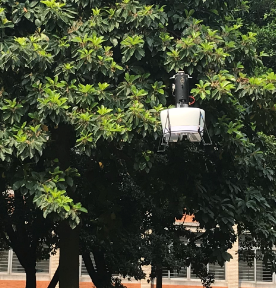
\includegraphics[scale=1]{Fig/DFUAV_f31.png}
	\caption{\label{fig_case1}测试测试测试}
\end{figure}
\begin{figure}[htbp]
	\centering	
	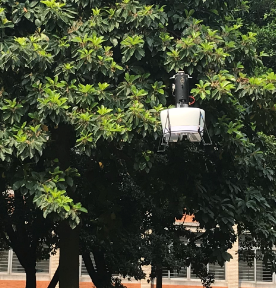
\includegraphics[scale=1]{Fig/DFUAV_f31.png}
	\caption{\label{fig_case2}测试测试测试}
\end{figure}
\begin{table}
	\caption{\label{DF_para1}测试测试测试}
	\centering{}%
	\small 
	\begin{tabular}{cccccc}
		\hline 
		参数符号 & 数值&参数符号 & 数值&参数符号 & 数值\tabularnewline
		\hline 
		$ A_x,A_y,A_z $  & $ 0.04082\,\text{m}^2 $ &$ \rho $        &$1.225\,\text{kg}/\text{m}^3$&$ I_b $           & $ 0.000029 $               \tabularnewline
		$ k_{\varpi} $   & $1.13342 \times 10^{-6}$& $ d_{\varpi} $ & $1.13342 \times 10^{-7}$ 	  &$k_{\delta} $     & $ 0.01495 $ 			      \tabularnewline
		$C_{D,x},C_{D,y}$& $ 0.43213 $             &$ C_{D,z} $     & $ 0.13421 $             	  &	$ q_a $ 	     & $ 1.49 $ 				  \tabularnewline
		$ l_{a} $        & $ -0.1121\,\text{m} $   & $ d_{ds} $     & $ 0.01495 $			  	  &$ d_{af} $        & $ 0.01495 $    			  \tabularnewline
		$ R $            & $ 0.11\,\text{m} $      &$ b $           & $ 2 $       			   	  &$ S $ 			 & $ 0.04082\,\text{m}^2 $    \tabularnewline
		$C_{l_{\alpha}}$ & $ 2.212\,/\text{rad} $  &$C_{l, \max } $ & $ 1.05 $ 				   	  &$ C_{l, \min } $  & $ -1.05 $ 				  \tabularnewline
		$ l_2 $          & $ 0.06647\,\text{m} $   &$ l_1 $         & $ 0.17078\,\text{m} $    	  &	$ m $ 		     & $ 1.53\,\text{kg} $ 		  \tabularnewline
		$ C_{d, o } $    & $ 0.9 $                 &$ C_{d, g } $   & $ 0.9 $					  &$ C_{duct} $      & $ 0.78497 $	 			  \tabularnewline
		$ I_x $          & $ 0.02548 $ 			   &$ I_y $         & $ 0.02550 $                 &$ I_z $			 & $ 0.00562 $ 				  \tabularnewline
		\hline 
	\end{tabular}	
\end{table}

\begin{table}
	\caption{\label{TDF_para2}测试测试测试}
	\centering{}%
	\small 
	%	\resizebox{\textwidth}{!}{
	\begin{tabular}{cccccc}
		\hline 
		参数符号 & 数值&参数符号 & 数值&参数符号 & 数值\tabularnewline
		\hline 
		$ I_x $ & $ 054593 $ &$ I_y $ & $ 0.017045 $& $ I_z$ & $ 0.049226 $ \tabularnewline
		$ l_{1} $ & $ 0.0808\,\text{m} $&$ l_{2} $ & $ 0.175\,\text{m} $ &$ l_3 $ & $ 0.06647\,\text{m} $ \tabularnewline 
		$ l_4 $ & $ 0.2415\,\text{m} $ &$ l_5 $ & $ 0.1085\,\text{m} $& $ m $ & $ 3.7\,\text{kg} $ \tabularnewline
		\hline 
	\end{tabular}	%}
\end{table}

\section{测试测试测试}
\subsection{测试测试测试}
%
测试测试测试测试测试测试测试测试测试测试测试测试测试测试测试测试测试测试测试测试测试测试测试测试测试测试测试测试测试测试测试测试测试测试测试测试测试测试测试测试测试测试测试测试测试测试测试测试测试测试测试测试测试测试测试测试测试测试测试测试测试测试测试测试测试测试测试测试测试测试测试测试测试测试测试测试测试测试测试测试测试测试测试测试测试测试测试测试测试测试测试测试测试测试测试测试测试测试测试测试测试测试



% 有多个附录

% %%%%%%%%%%%%%%%%%%%此部分为附录1环境代码,是比较笨的方法来适应论文撰写规范%%%%%%%%%%%%%%%%%%%%%%%%%%%%%%%%%%%%%%
%新增附录时只需要将\setcounter{chapter}{X}以及\chapter{附\texorpdfstring{\quad}{}录 X}中相应的X更改为
%相应的数字,如果只有一个附录,则选用appendix
%%%%%%%%%%%%%%%%%%%%%%%%%%%%%%%%%%%%%%%%%%%%%%%%%%%%%%%%%%%%%%%%%%%%%%%%%%%%%%%%%%%%%%%%%%%%%%%%%%%%%%%%%%%%
\setcounter{chapter}{1} %从1开始编号
\setcounter{section}{0}
\setcounter{equation}{0}
\setcounter{table}{0}   
\setcounter{figure}{0}
\chapter{附\texorpdfstring{\quad}{}录 1} %附录1
%%%%%%%%%%%%%%%%%%%%%%%%%%%%%%%%%%%%%%%%%%%%%%%%%%%%%%%%%%%%%%%%%%%%%%%%%%%%%%%%%%%%%%%%%%%%%%%%%%%%%%%%
%%%%%%%%%%%%以下为用户代码,用于撰写您的论文%%%%%%%%%%%%%%%%%%%%%%%%%%%%%%%%%%%%%%%%%%%%%%%%%%%%%%%%%%%%%%

在论文撰写规范中,下面两段话让人费解:

\begin{enumerate}
	\item 	对需要收录于学位论文中但又不适合书写于正文中的附加数据、方案、资料、详细公式推导、计算机程序、统计表、注释等有特色的内容,可做为附录排写,序号采用“附录1”、“附录2”等。	
	\item	公式序号按章编排,如第一章第一个公式序号为“(1-1)”,附录2中的第一个公式为“(2-1)”等。
\end{enumerate}

论文撰写规范要求的附录和通常书籍上使用附录A、附录B等编号的不一样,容易和正文混淆。特殊的要求和代码的耦合,使我不得不使用比较笨的方法来设计附录部分的模板。这部分还需要有附录需求的同学来完善,为了目录中美观且不命名冲突,还是不在附录使用图表。


\section{测试一级标题 section}
\subsection{测试二级标题 subsection}
\subsubsection{测试三级标题 subsubsection}
%
测试测试测试测试测试测试测试测试测试测试测试测试测试测试测试测试测试测试测试测试测试测试测试测试测试测试测试测试测试测试测试测试测试测试测试测试测试测试测试测试测试测试测试测试测试测试测试测试测试测试测试测试测试测试测试测试测试测试测试测试测试测试测试测试测试测试测试测试测试测试测试测试测试测试测试测试测试测试测试测试测试测试测试测试测试测试测试测试测试测试测试测试测试测试测试测试测试测试测试测试测试测试测试测试测试测试测试测试测试测试测试测试测试测试测试测试测试测试测试测试测试测试测试测试测试测试测试测试测试测试测试测试测试测试测试测试测试测试测试测试测试测试测试测试测试测试测试测试测试测试测试测试测试
\begin{align}
\left\{\begin{array}{l}
\dot{v}_{1}(t)=v_{2}(t) \\
\dot{v}_{2}(t)=R^{2}\left(-\zeta_{1}\left[v_{1}(t)-v_c(t)\right]^{\alpha}-\zeta_{2}\left[\dfrac{v_{2}(t)}{R}\right]^{\beta}\right)
\end{array}\right.	
\end{align}

\begin{align}
\left\{\begin{array}{l}
\dot{v}_{1}(t)=v_{2}(t) \\
\dot{v}_{2}(t)=R^{2}\left(-\zeta_{1}\left[v_{1}(t)-v_c(t)\right]^{\alpha}-\zeta_{2}\left[\dfrac{v_{2}(t)}{R}\right]^{\beta}\right)
\end{array}\right.	
\end{align}
% \begin{figure}[htbp]
% 	\centering	
% 	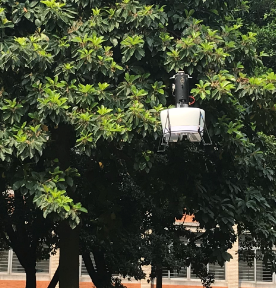
\includegraphics[scale=1]{Fig/DFUAV_f31.png}
% 	\caption{\label{fig_case1}测试测试测试}
% \end{figure}
% \begin{figure}[htbp]
% 	\centering	
% 	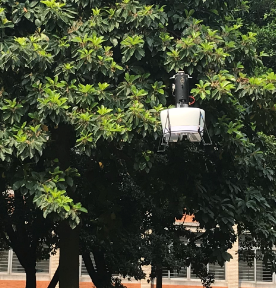
\includegraphics[scale=1]{Fig/DFUAV_f31.png}
% 	\caption{\label{fig_case2}测试测试测试}
% \end{figure}
% \begin{table}
% 	\caption{\label{DF_para1}测试测试测试}
% 	\centering{}%
% 	\small 
% 	\begin{tabular}{cccccc}
% 		\hline 
% 		参数符号 & 数值&参数符号 & 数值&参数符号 & 数值\tabularnewline
% 		\hline 
% 		$ A_x,A_y,A_z $  & $ 0.04082\,\text{m}^2 $ &$ \rho $        &$1.225\,\text{kg}/\text{m}^3$&$ I_b $           & $ 0.000029 $               \tabularnewline
% 		$ k_{\varpi} $   & $1.13342 \times 10^{-6}$& $ d_{\varpi} $ & $1.13342 \times 10^{-7}$ 	  &$k_{\delta} $     & $ 0.01495 $ 			      \tabularnewline
% 		$C_{D,x},C_{D,y}$& $ 0.43213 $             &$ C_{D,z} $     & $ 0.13421 $             	  &	$ q_a $ 	     & $ 1.49 $ 				  \tabularnewline
% 		$ l_{a} $        & $ -0.1121\,\text{m} $   & $ d_{ds} $     & $ 0.01495 $			  	  &$ d_{af} $        & $ 0.01495 $    			  \tabularnewline
% 		$ R $            & $ 0.11\,\text{m} $      &$ b $           & $ 2 $       			   	  &$ S $ 			 & $ 0.04082\,\text{m}^2 $    \tabularnewline
% 		$C_{l_{\alpha}}$ & $ 2.212\,/\text{rad} $  &$C_{l, \max } $ & $ 1.05 $ 				   	  &$ C_{l, \min } $  & $ -1.05 $ 				  \tabularnewline
% 		$ l_2 $          & $ 0.06647\,\text{m} $   &$ l_1 $         & $ 0.17078\,\text{m} $    	  &	$ m $ 		     & $ 1.53\,\text{kg} $ 		  \tabularnewline
% 		$ C_{d, o } $    & $ 0.9 $                 &$ C_{d, g } $   & $ 0.9 $					  &$ C_{duct} $      & $ 0.78497 $	 			  \tabularnewline
% 		$ I_x $          & $ 0.02548 $ 			   &$ I_y $         & $ 0.02550 $                 &$ I_z $			 & $ 0.00562 $ 				  \tabularnewline
% 		\hline 
% 	\end{tabular}	
% \end{table}

% \begin{table}
% 	\caption{\label{TDF_para2}测试测试测试}
% 	\centering{}%
% 	\small 
% 	%	\resizebox{\textwidth}{!}{
% 	\begin{tabular}{cccccc}
% 		\hline 
% 		参数符号 & 数值&参数符号 & 数值&参数符号 & 数值\tabularnewline
% 		\hline 
% 		$ I_x $ & $ 054593 $ &$ I_y $ & $ 0.017045 $& $ I_z$ & $ 0.049226 $ \tabularnewline
% 		$ l_{1} $ & $ 0.0808\,\text{m} $&$ l_{2} $ & $ 0.175\,\text{m} $ &$ l_3 $ & $ 0.06647\,\text{m} $ \tabularnewline 
% 		$ l_4 $ & $ 0.2415\,\text{m} $ &$ l_5 $ & $ 0.1085\,\text{m} $& $ m $ & $ 3.7\,\text{kg} $ \tabularnewline
% 		\hline 
% 	\end{tabular}	%}
% \end{table}

\section{测试测试测试}
\subsection{测试测试测试}
%
测试测试测试测试测试测试测试测试测试测试测试测试测试测试测试测试测试测试测试测试测试测试测试测试测试测试测试测试测试测试测试测试测试测试测试测试测试测试测试测试测试测试测试测试测试测试测试测试测试测试测试测试测试测试测试测试测试测试测试测试测试测试测试测试测试测试测试测试测试测试测试测试测试测试测试测试测试测试测试测试测试测试测试测试测试测试测试测试测试测试测试测试测试测试测试测试测试测试测试测试测试测试

 %附录1
% %%%%%%%%%%%%%%%%%%%此部分为附录1环境代码,是比较笨的方法来适应论文撰写规范%%%%%%%%%%%%%%%%%%%%%%%%%%%%%%%%%%%%%%
%新增附录时只需要将\setcounter{chapter}{X}以及\chapter{附\texorpdfstring{\quad}{}录 X}中相应的X更改为相应的数字
\setcounter{chapter}{2} %从2开始编号
\setcounter{section}{0}
\setcounter{equation}{0}
\setcounter{table}{0}   
\setcounter{figure}{0}
\chapter{附\texorpdfstring{\quad}{}录 2} %附录2
%%%%%%%%%%%%%%%%%%%%%%%%%%%%%%%%%%%%%%%%%%%%%%%%%%%%%%%%%%%%%%%%%%%%%%%%%%%%%%%%%%%%%%%%%%%%%%%%%%%%%%%%
%%%%%%%%%%%%以下为用户代码,用于撰写您的论文%%%%%%%%%%%%%%%%%%%%%%%%%%%%%%%%%%%%%%%%%%%%%%%%%%%%%%%%%%%%%%

在论文撰写规范中,下面两段话让人费解:

\begin{enumerate}
	\item 	对需要收录于学位论文中但又不适合书写于正文中的附加数据、方案、资料、详细公式推导、计算机程序、统计表、注释等有特色的内容,可做为附录排写,序号采用“附录1”、“附录2”等。	
	\item	公式序号按章编排,如第一章第一个公式序号为“(1-1)”,附录2中的第一个公式为“(2-1)”等。
\end{enumerate}

论文撰写规范要求的附录和通常书籍上使用附录A、附录B等编号的不一样,上述要求最终的效果是这些编号容易和正文的混淆。特殊的要求和代码的耦合,使我不得不使用比较笨的方法来设计附录部分的模板。这部分还需要有附录需求的同学来完善,为了目录中美观且不命名冲突,还是不在附录使用图表。

\section{测试测试测试}
\subsection{测试测试测试}
%
测试测试测试测试测试测试测试测试测试测试测试测试
\begin{align}
\left\{\begin{array}{l}
\dot{v}_{1}(t)=v_{2}(t) \\
\dot{v}_{2}(t)=R^{2}\left(-\zeta_{1}\left[v_{1}(t)-v_c(t)\right]^{\alpha}-\zeta_{2}\left[\dfrac{v_{2}(t)}{R}\right]^{\beta}\right)
\end{array}\right.	
\end{align}
\begin{align}
\left\{\begin{array}{l}
\dot{v}_{1}(t)=v_{2}(t) \\
\dot{v}_{2}(t)=R^{2}\left(-\zeta_{1}\left[v_{1}(t)-v_c(t)\right]^{\alpha}-\zeta_{2}\left[\dfrac{v_{2}(t)}{R}\right]^{\beta}\right)
\end{array}\right.	
\end{align}
% 注释掉图表:
% \begin{figure}[htbp]
% 	\centering	
% 	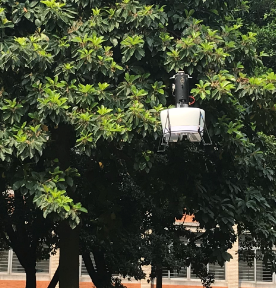
\includegraphics[scale=1]{Fig/DFUAV_f31.png}
% 	\caption{\label{fig_c1}测试测试测试}
% \end{figure}
% \begin{figure}[htbp]
% 	\centering	
% 	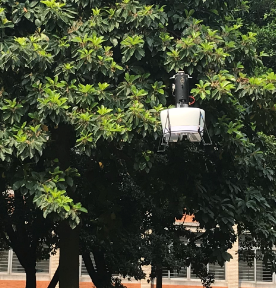
\includegraphics[scale=1]{Fig/DFUAV_f31.png}
% 	\caption{\label{fig_c2}测试测试测试}
% \end{figure}
% \begin{table}
% 	\caption{\label{DF_p1}测试测试测试}
% 	\centering{}%
% 	\small 
% 	\begin{tabular}{cccccc}
% 		\hline 
% 		参数符号 & 数值&参数符号 & 数值&参数符号 & 数值\tabularnewline
% 		\hline 
% 		$ A_x,A_y,A_z $  & $ 0.04082\,\text{m}^2 $ &$ \rho $        &$1.225\,\text{kg}/\text{m}^3$&$ I_b $           & $ 0.000029 $               \tabularnewline
% 		$ k_{\varpi} $   & $1.13342 \times 10^{-6}$& $ d_{\varpi} $ & $1.13342 \times 10^{-7}$ 	  &$k_{\delta} $     & $ 0.01495 $ 			      \tabularnewline
% 		$C_{D,x},C_{D,y}$& $ 0.43213 $             &$ C_{D,z} $     & $ 0.13421 $             	  &	$ q_a $ 	     & $ 1.49 $ 				  \tabularnewline
% 		$ l_{a} $        & $ -0.1121\,\text{m} $   & $ d_{ds} $     & $ 0.01495 $			  	  &$ d_{af} $        & $ 0.01495 $    			  \tabularnewline
% 		$ R $            & $ 0.11\,\text{m} $      &$ b $           & $ 2 $       			   	  &$ S $ 			 & $ 0.04082\,\text{m}^2 $    \tabularnewline
% 		$C_{l_{\alpha}}$ & $ 2.212\,/\text{rad} $  &$C_{l, \max } $ & $ 1.05 $ 				   	  &$ C_{l, \min } $  & $ -1.05 $ 				  \tabularnewline
% 		$ l_2 $          & $ 0.06647\,\text{m} $   &$ l_1 $         & $ 0.17078\,\text{m} $    	  &	$ m $ 		     & $ 1.53\,\text{kg} $ 		  \tabularnewline
% 		$ C_{d, o } $    & $ 0.9 $                 &$ C_{d, g } $   & $ 0.9 $					  &$ C_{duct} $      & $ 0.78497 $	 			  \tabularnewline
% 		$ I_x $          & $ 0.02548 $ 			   &$ I_y $         & $ 0.02550 $                 &$ I_z $			 & $ 0.00562 $ 				  \tabularnewline
% 		\hline 
% 	\end{tabular}	
% \end{table}

% \begin{table}
% 	\caption{\label{TDF_p2}测试测试测试}
% 	\centering{}%
% 	\small 
% 	%	\resizebox{\textwidth}{!}{
% 	\begin{tabular}{cccccc}
% 		\hline 
% 		参数符号 & 数值&参数符号 & 数值&参数符号 & 数值\tabularnewline
% 		\hline 
% 		$ I_x $ & $ 054593 $ &$ I_y $ & $ 0.017045 $& $ I_z$ & $ 0.049226 $ \tabularnewline
% 		$ l_{1} $ & $ 0.0808\,\text{m} $&$ l_{2} $ & $ 0.175\,\text{m} $ &$ l_3 $ & $ 0.06647\,\text{m} $ \tabularnewline 
% 		$ l_4 $ & $ 0.2415\,\text{m} $ &$ l_5 $ & $ 0.1085\,\text{m} $& $ m $ & $ 3.7\,\text{kg} $ \tabularnewline
% 		\hline 
% 	\end{tabular}	%}
% \end{table} %附录2
%%%%%%%%%%%%%%%%%%%
\chapter{攻读博士/硕士学位期间取得的研究成果} %博士/硕士记得选其一
\pubfont % 论文撰写规范里,这章是5号宋体,\pubfont 设置字号为5号了。但其实很多论文用小四号也OK。
一、已发表(包括已接受待发表)的论文,以及已投稿、或已成文打算投稿、或拟成文投稿的论文情况\underline{\textbf{(只填写与学位论文内容相关的部分):}}
\begin{table}
	\centering{}%
	\pubfont
	\begin{longtable}{|>{\centering}m{0.5cm}|m{1.8cm}|>{\centering}m{2.8cm}|>{\centering}m{2.5cm}|>{\centering}m{2.2cm}|>{\centering}m{2.cm}|>{\centering}m{1cm}|}
		\hline
		\textbf{序号} & \textbf{作者(全体作者,按顺序排列)} & \textbf{题 目}    & \textbf{发表或投稿刊物名称、级别} & \textbf{发表的卷期、年月、页码} & \textbf{与学位论文哪一部分(章、节)相关} & \textbf{被索引收录情况}\tabularnewline
		\hline
		1           & redfu                   & 在LaTeX中有三种基本的列举 & acm                   & 2000.04,100(10)      & 第三章                       & 已见刊  \tabularnewline
		\hline
		2           &                         &                 &                       &                      &                           & \tabularnewline
		\hline
	\end{longtable}
\end{table}

注:在“发表的卷期、年月、页码”栏:

1.如果论文已发表,请填写发表的卷期、年月、页码;

2.如果论文已被接受,填写将要发表的卷期、年月;

3.以上都不是,请据实填写“已投稿”,“拟投稿”。

不够请另加页。

二、与学位内容相关的其它成果(包括专利、著作、获奖项目等)



%注:这部分一言难尽,我努力了很久都没有把这个表做好。感觉学校给的这个表的模板非常反人类。看国外大学的博士论文,那种像参考文献著录信息那样一行一行的,比较美观。而这个框框很难放文字进去。

\normalsize % \normalsize可以将下文调回和正文一样的字号,这个随个人喜好。注释掉的话,致谢就就跟随《攻读博士/硕士学位期间取得的研究成果》的字号。 %成果
\chapter{致\texorpdfstring{\quad}{}谢}
南柯一梦,三载华工。时光如雨丝轻落,花影斑驳,往昔的点滴在心头悄然流转。回望这段旅程,我或许并非传统意义上的“好学生”,但人生的意义,常常藏在那些不被定义的时刻里。幸运的是,在这段不算璀璨的研究生岁月里,我遇见了许多温暖的人,他们的陪伴与点拨,让这段旅途成为我生命中不可磨灭的印记。

首先,衷心感谢我的导师,周嘉嘉老师。与周老师的相识虽短,却深刻如春风化雨。有限的时光里,老师对我的学术研究给予了极大的帮助,从论文选题到中期检查,再到最后的预答辩,每一步都耐心指导。他治学严谨,热忱专注,在他身上我看见了学者的风骨,也学会了如何在迷茫中寻找方向。

其次,感谢师门的每一位同学。感谢袁爽、操能杰等师兄师姐在学术上的悉心帮助。正是因为有这样一个团结、优秀的课题组,我才能在学术的森林中不至于迷失。同行者的陪伴,让孤独的求索变得温暖而有力。

再者,感激我的家人和朋友们。你们在我最迷茫时给予我安慰,在我最无助时给予我支持,在我最需要时给予我鼓励。你们的爱与陪伴,是我心灵深处最坚实的依靠。

最后,我要感谢那个永不言弃的自己,我始终坚信即使是西西弗斯,也能在日复一日的推石中找到属于自己的意义。
\begin{flushright}
  傅星源\\
  2025年8月20日于华园
\end{flushright}

 %致谢
% 插入外部PDF文件为新的一页,需使用pdfpages宏包(请确保导言区已\usepackage{pdfpages})
% \cleardoublepage

\includepdf[pages=-]{cover_file/pingyu.pdf} % 将"yourfile.pdf"替换为你的PDF文件名,pages=-表示插入全部页面

\end{document}
